%------------ Hinweise --------------------------------------------
% Um das fertige Dokument zu erstellen, wie folgt vorgehen:
% 1. pdflatex Diplomarbeit.tex
% 2. makeindex Diplomarbeit.idx -s Diplomarbeits.ist -t Diplomarbeit.nlg -o Diplomarbeit.nls 
% (Alternativ sollte auch makeindex Diplomarbeit funktionieren)
% 3. makeglossaries Diplomarbeit
% 4. biber Diplomarbeit
% 5. pdflatex Diplomarbeit.tex
%
% Das ganze lässt sich in diversen Editoren (z.B. TeXnicCenter) in fertigen Profilen 
% speicheren bzw. durch leichte Abwandlung schon vorhandener Profile erreichen. Beim
% allerersten Aufruf ist der ganze Ablauf zweimal nötig, um alle Referenzen usw.
% aufzulösen!
%
% Die hier geladenene Pakete stellen viele grundlegende Funktionen zur Verfügung. 
% Alles weitere bitte selbst hinzufügen.


%------------ Header --------------------------------------------
\documentclass[%
  ngerman,%
  BCOR=0mm,
  cdgeometry=yes,
  numbers=noenddot,
  paper=a4,
  listof=totoc, bibliography=totoc,
]{tudscrreprt}
\iftutex
  \usepackage{fontspec}
\else
  \usepackage[T1]{fontenc}
  \usepackage[ngerman=ngerman-x-latest]{hyphsubst}
\fi
\setcounter{secnumdepth}{4} % Ueberschriften bis 4. Ebene nummeriert
\setcounter{tocdepth}{4} 		% Ueberschriften bis 4. Ebene in Inhaltsverzeichnis


%------------ Deutsche Anpassungen und Schrift ------------------------------------
\usepackage[ngerman]{babel}
\usepackage[style=numeric, sorting=none, backend=biber]{biblatex}
%\usepackage[style=ieee, sorting=none, backend=biber]{biblatex}
\usepackage[T1]{fontenc}			 % Font-Encoding, welches Umlaute unterstützt
\usepackage[utf8]{inputenc} % Tex-Dateien werden ANSI-Kodiert erwartet. Umlaute können direkt im Tex-Dokument verwendet werden
\usepackage{textcomp}
\usepackage{gensymb}

\usepackage{csquotes}		% Für biblatex
\usepackage{lmodern}     			 % Umfangreiche und hübsche Schriftart

\usepackage{caption}    			 % Captions außerhalb von floats erstellen
\usepackage{upgreek}		 			 % Griechische Einheiten nicht kursiv darstellen

% \usepackage[default]{opensans}
\usepackage[ngerman]{babel}							% Deutsche Bezeichner
\addto\captionsngerman{%								% Macht aus der Beschriftung Abbildung --> Abb.
	\renewcommand{\figurename}{Abb.}%			%
	\renewcommand{\tablename}{Tab.}%			%
}
\babelhyphenation[ngerman]{pa-ral-lel}
  

%------------ Grafiken und Abbildungen --------------------------------------------
\usepackage[pdftex]{graphicx} % Grafiken in pdfLaTeX
\usepackage{float}						% Das Bild mit [ht] wenn möglich an der Stelle wie im Tex-Dokument ausgeben.
\pdfinclusioncopyfonts=1 			% Richtige Darstellung der in Matlab erstellten Axenbeschriftungen

\usepackage{subcaption}				% Mehrere Bilder in einer Figure Umgebung mit separaten Bildunterschriften

\renewcommand{\thefigure}{\arabic{chapter}.\arabic{figure}}		% Abbildungsnummerierung im Format Kapitel.Nummer


%------------ Formeldarstellung --------------------------------------------
\usepackage{amsmath}     % Mathematische Befehle
\usepackage{amssymb}     % Erweiterte math. Symbole lädt implizit amsfonts
\usepackage{amstext}		 % \text{} im math-modus
\usepackage{siunitx}		 % Korrektes Verwendung von Einheiten mit \SI{Zahl}{\einheit}


%------------ Zeilenabstand und Absätze --------------------------------------------
\usepackage{setspace}		% Zeilenabstand einstellen
%\singlespacing					% 1-zeilig (Standard)
\onehalfspacing					% 1,5-zeilig
%\doublespacing					% 2-zeilig

\setlength{\parindent}{1em}	% Einrücktiefe von neuen Absätzen


%------------ Seitenlayout --------------------------------------------
\usepackage{geometry}                % Ändern der Seitengeometrie. 

%------------ Header und Footer --------------------------------------------
% Fuß- und Kopfseparierungslinie im scrlayer style. Im plain.scrlayer style nur eine Fußlinie
\usepackage[headsepline=0.5pt,footsepline=0.5pt,plainfootsepline]{scrlayer-scrpage}

\KOMAoptions{onpsinit=\setstretch{1.2}} % Verhindert die Beeinflussung von header und footer durch spacing Umgebungen
% \pagestyle{scrheadings}

\ohead{\leftmark}		% Kapitel außen in der Kopfzeile (bei Einsitigem Druck heißt das rechts)
\ifoot{Masterarbeit Antonia Gerdes}

% Seitennummer außen in Fußzeile (wird für Kaptielüberschriften und dergleichen automatisch verwendet)
% '*' heißt, das die Einstellung auch im plain style gilt
\ofoot*{\thepage}
\cfoot*{}			% Im scrlayer Style voreingestellte Seitennummer in der Mitte unten entfernen.
\chead*{} 		% Siehe \cfoot, allerdings für den Header
\setkomafont{pageheadfoot}{\normalsize} 	% Normale Schrift, nicht kursiv wie voreingestellt


%------------ Links im PDF-Dokument -------------------------------------------
\usepackage[hypertexnames=false]{hyperref}%Verlinkungen des TOC im Dokument machen (3xkompilieren)
\hypersetup{
  hypertexnames=false,   % korrekte Numerierung wg. arabisch und römisch
  colorlinks=true,       % Links werden farbig und nicht umrandet
  linkcolor=black,       % Linkfarbe
  citecolor=black,       % Farbe für Zitate
  urlcolor=black,        % Farbe für Webadressen
  bookmarksopen=true,    % im Reader wird Gliederung angezeigt
 %pdfpagelabels=true,    % Nummerierung für PDF-Datei
            } 
						
						
%------------ Abkürzungsverzeichnis --------------------------------------------
\usepackage[acronym,toc,nomain,nonumberlist,nopostdot, nogroupskip]{glossaries}
\renewcommand{\glsnamefont}[1]{\textbf{#1}}
\makeglossaries

%------------ Selbst hinzugefügte Packages -----------------------------------
\usepackage{pdflscape}
\usepackage{booktabs} % Für bessere Tabellen
\usepackage{multirow} % Für Mehrzeilen
\usepackage{array}    % Für Spaltenformatierung
\usepackage{makecell} % Für Umbrüche innerhalb von Zellen in Tabellen
\usepackage{adjustbox}% Um Tabellen zu resizen

%------------ Weitere Packages --------------------------------------------
\usepackage{url}					% Richtige Onlinezitierung

\usepackage{pdfpages}			% Um pdf Dateien dem Latex-dokument EINFACH hinzuzufügen 

\usepackage{color}				% Farbige Markierungen setzen\colorbox{yellow}{hervorgehoben}
\definecolor{dunkelgrau}{rgb}{0.8,0.8,0.8} % Define user colors using the RGB model
\definecolor{hellgrau}{rgb}{0.90,0.90,0.90}
\usepackage{colortbl}			% Um die Farben in Tabellen zu verwenden


\usepackage{remreset} 		% Paket um den Counter für die Fussnoten zu setzen da diese Ansonsten mit jedem neuen Kapitel 
													% wieder von 1 beginnen

\makeatletter           	% Ändern der Vorlage erlauben
\setlength{\@fptop}{0pt}	% floats oben plazieren
\@addtoreset{figure}{chapter}						%Rücksetzen der Abbildungsnummerierung mit jedem neuen Kapitel
\@removefromreset{footnote}{chapter}		%Fussnoten vom Rücksetzen bei Beginn eines neuen Kapitel ausschließen
\makeatother

\Ifpdfoutput{																																			% PDF-Eigenschaften festlegen
    \hypersetup {																																	%
        pdftitle={Titel der Arbeit},	% Titel
        pdfsubject={Masterarbeit},																								% Thema
        pdfauthor={Antonia Gerdes},																								%	Autor
        pdfkeywords={Masterarbeit, TU DD, Level-Set, Segmentierung}								%	Schlüsselwörter
    }
}{}

\pdfminorversion=6
\DeclareMathOperator{\e}{e}

\usepackage{listings}		% Quellcode Listings mit Syntax-Highlighting \begin{lstlisting}...\end{lstlisting}

\usepackage{scrhack}		% Verbessert Kompatibilität zwischen KOMA-Script und anderen Packages (float, hyperrref etc.)

\makeindex							% Let Latex output a .idx file for makeindex

% Weitere benötigte Packages entweder hier hin oder in config.tex 
% (z.B. falls Reihenfolge zu dort definierten Paketen wichtig ist)

\graphicspath{ {./Bilder/} }
\addbibresource{library.bib} % Literaturverzeichnis

\newacronym{EKG}{EKG}{Elektrokardiogramm}
\newacronym{AV-Knoten}{AV-Knoten}{Atrioventrikularknoten}
\newacronym[description=Vorhofflimmern]{VHF}{VHF}{Vorhofflimmern}
\newacronym{ML}{ML}{Machine Learning}
\newacronym{DL}{DL}{Deep Learning}
\newacronym{SVM}{SVM}{Support Vector Machine}
\newacronym{DTE}{DTE}{Decision Tree Ensemble}
\newacronym[description=Convolutional Neural Network, plural=CNNs]{CNN}{CNN}{Convolutional Neural Network}
\newacronym[description=Artificial Neural Network, plural=ANNs]{ANN}{ANN}{Artificial Neural Network}
\newacronym[description=Feed Forward Neural Network, plural=FFNNs]{FFNN}{FFNN}{Feed Forward Neural Network}
\newacronym{AUC}{AUC}{Area Under Curve}
\newacronym{ROC}{ROC}{Receiver-Operating-Characteristic}
\newacronym[description=Deep Neural Network, plural=DNNs, longplural=Deep Neural Networks]{DNN}{DNN}{Deep Neural Network}
\newacronym{SR}{SR}{Sinusrhythmus}
\newacronym[description=Residual Network, plural=ResNets, longplural=Residual Networks]{ResNet}{ResNet}{Residual Network}
\newacronym{ReLU}{ReLu}{Rectified Linear Unit}
\newacronym{kNN}{kNN}{k Nearest Neighbor}
\newacronym{HRV}{HRV}{Herzratenvariabilität}
\newacronym{2DSW}{2DSW}{2-Dimensional Signal Warping}
\newacronym{SQI}{SQI}{Signal Quality Indices}
\newacronym[description=True Positives]{TP}{TP}{True Positives}
\newacronym{FP}{FP}{False Positives}
\newacronym{TN}{TN}{True Negatives}
\newacronym{FN}{FN}{False Negatives}
\newacronym[description=ventrikuläre Extrasystole, plural=VES]{VES}{VES}{ventrikulären Extrasystolen}
\newacronym[description=supraventrikuläre Extrasystole, plural=SVES]{SVES}{SVES}{supraventrikulären Extrasystolen}
\newacronym[description=Vorhofextrasystole, plural=VoES]{VoES}{VoES}{Vorhofextrasystolen}
\newacronym[description=early afterdepolarization, plural=EADs]{EAD}{EAD}{early afterdepolarization}
\newacronym[description=delayed afterdepolarization, plural=DADs]{DAD}{DAD}{delayed afterdepolarization}
\newacronym{MLP}{MLP}{Multilayer Perceptron}
\newacronym{CPSC2018}{CPSC2018}{China Physiological Signal Challenge 2018}
\newacronym{SHDB-AF}{SHDB-AF}{Saitama Heart Database Atrial Fibrillation}
\newacronym{KI}{KI}{künstliche Intelligenz}
\newacronym{PPG}{PPG}{Photoplethysmographie}
\newacronym[description=Domain Adversarial Neural Network, plural=DANNs]{DANN}{DANN}{Domain Adversarial Neural Network}
\newacronym{DAp}{DAp}{Domain Adaptation}
\newacronym{DG}{DG}{Domain Generalization}
\newacronym{FC}{FC}{Fully Connected}
\newacronym{LSTM}{LSTM}{Long Short-Term Memory}
\newacronym{GRL}{GRL}{Gradient Reversal Layer}
\newacronym{GAP}{GAP}{Global Average Pooling}
\newacronym[description=Generative Adversarial Network, plural=GANs]{GAN}{GAN}{Generative Adversarial Network}
\newacronym{UCR}{UCR}{University of California, Riverside}
\newacronym{UEA}{UEA}{University of East Anglia}
\newacronym{HPC}{HPC}{High Performance Computer}




%Beispiele

\newacronym[description=fetales Elektrokardidogramm]{fEKG}{fEKG}{fetalen EKG}
\newacronym[description=maternales EKG]{mEKG}{mEKG}{maternale EKG}
\newacronym[description=abdominal aufgenommenes Signal, plural=abdmSign]{abdmSig}{abdmSig}{abdominal aufgenommenen Signal}
\newacronym{EHG}{EHG}{Elektrohystereogramm}
\newacronym{EMG}{EMG}{Elektromyogram}
\newacronym[description=Institut für Biomedizinische Technik der TU Dresden]{IBMT}{IBMT}{Institut für Biomedizinische Technik}
\newacronym{rMess}{$r_\mathrm{Mess}$}{Messrauschen}
\newacronym{rNetz}{$r_\mathrm{Netz}$}{Netzrauschen}
\newacronym{bWa}{bWa}{Baselinewander}
\newacronym{CTG}{CTG}{Kardiotokographie}
\newacronym{fHR}{fHR}{fetale Herzrate}
\newacronym{fHRV}{fHRV}	{Variabilität der fetalen Herzrate}
\newacronym[description=Kalman Filter]{KF}{KF}{Kalman Filters}
\newacronym[description=Extended Kalman Filter]{EKF}{EKF}{Extended Kalman Filter}
\newacronym[description=Signal-Rausch-Verhältnis]{SNR}{SNR}{Signal-Rausch-Verhältnis}
\newacronym[plural=DGLn, firstplural=Differentialgleichungen (DGLn)]{DGL}{DGL}{Differentialgleichung}



 % Definitionsliste für Acronyme


%------------ Dokumentbeginn ----------------------------------------------
\begin{document}

%---- Deckblatt					
% % % % % INFO  % % % % %
\faculty{Fakultät Elektrotechnik und Informationstechnik}
%\department{Name der Einrichtung an der Fakult\"at}
\institute{Institut für Biomedizinische Technik}
%\chair{Chair of Communications Theory}

\title{Entwicklung eines robusten Deep Learning Ansatzes zur Detektion von Vorhofflimmern in mobilen EKG-Aufnahmen}

% Diplomarbeit:
\thesis{Masterarbeit} 
\graduation[M.Sc.]{Master of Science}

% Studienarbeit:
% \thesis{student} 


\author{Antonia Gerdes} %
\dateofbirth{21.02.1996}
\placeofbirth{Wilhelmshaven}

\professor{Prof. Dr.-Ing. habil. H. Malberg}
\referee{Prof. Dr.-Ing. habil. H. Malberg \and Prof. Dr.-Ing. Raimund Dachselt} % Gutachter (nur bei DA!)
\supervisor{Dr.-Ing. Martin Schmidt
 \and Dipl.-Wi.-Ing. Alexander Hammer}
% \issuedate{1.4.2021}
% \duedate{1.10.2021}

\date{27. Februar 2025}

\makecover
\maketitle

 % Eigene Daten in Deckblatt.tex anpassen


%---- Aufgabenstellung

\includepdf{Aufgabenstellung.pdf}  % Einbinden einer externen pdf in Latex

\pagenumbering{roman} % römische Nummerierung bis zur Einleitung
\setcounter{page}{2} % Aufgabenstellung war ja schon Seite 1


%---- Selbstständigkeitserklärung 


\chapter*{Selbstständigkeitserklärung}

Hiermit versichere ich, dass ich die vorliegende Arbeit mit dem Titel \textit{Entwicklung eines robusten Deep Learning Ansatzes zur Detektion von Vorhofflimmern in mobilen EKG-Aufnahmen} selbstständig und ohne unzulässige Hilfe Dritter verfasst habe. Es wurden keine anderen als die in der Arbeit angegebenen Hilfsmittel und Quellen benutzt. Die wörtlichen und sinngemäß übernommenen Zitate habe ich als solche kenntlich gemacht. Mir ist bekannt, dass die Nichteinhaltung dieser Erklärung zum nachträglichen Entzug des Hochschulabschlusses führen kann.\\
\\
\\
\noindent
Antonia Gerdes \\
Dresden, 27. Februar 2025 \newpage


%---- Abstrakt
\chapter*{Abstrakt}

Vorhofflimmern ist eine der häufigsten Herzrhythmusstörungen und bringt ein erhöhtes Schlaganfallrisiko mit sich, was zu bleibenden Schäden bis hin zum vorzeitigen Tod führen kann. Die frühzeitige Detektion von Vorhofflimmern ist wünschenswert, da es andernfalls zur Chronifizierung kommen kann.
Der Goldstandard zur Diagnose von Vorhofflimmern ist das 12-Kanal-EKG, welches durch medizinisches Fachpersonal interpretiert wird. Um das lediglich phasenweise auftretende paroxysmale Vorhofflimmern zu diagnostizieren, ist ein Langzeit-EKG nötig, welches mittels mobilen EKG-Patches aufgezeichnet werden kann. 

Die manuelle Auswertung dieser EKGs ist jedoch ressourcenintensiv, weshalb eine automatisierte Auswertung mittels Deep Learning-Algorithmen nötig ist. Mobile EKG-Patches haben außerdem eine reduzierte Kanalanzahl und die Signalmorphologie unterscheidet sich von der der 12-Kanal-EKGs. Aufgrund dieser Abweichungen sind bereits vorhandene Klassifikationsansätze auf Aufnahmen mobiler EKG-Patches nur begrenzt übertragbar. 
Um dieses Problem zu lösen, wird in dieser Arbeit ein Deep Learning-basierter Ansatz zur Detektion von Vorhofflimmern auf Basis von 12-Kanal-EKGs entwickelt, welcher robust gegen signalmorphologische Veränderungen ist. 

Das entwickelte gewichtete Ensemble aus 5 Domain Adversarial Neural Networks erreicht einen F1-Score von bis zu 0,962 auf einem Testdatensatz aus 12-Kanal-EKGs, sowie einen Recall von bis zu 0,955 und eine Specificity von bis zu 0,973.
Auf Aufnahmen aus dem TIMELY-Projekt, welche mittels mobiler EKG-Patches aufgezeichnet wurden, erreicht das Ensemble einen F1-Score von bis zu 0,986, sowie einen Recall von bis zu 1,00 und eine Specificity von bis zu 0,979.
	\newpage			% deutsch  	Kurzfassung
	
\chapter*{Abstract}

Atrial fibrillation is one of the most common cardiac arrhythmias and leads to a higher risk of stroke, which can cause permanent damage and premature death. The early detection of atrial fibrillation is desirable, as untreated atrial fibrillation can become chronic. The gold standard for atrial fibrillation diagnosis is the 12-lead ECG, which is interpreted by medical personnel. Because paroxysmal atrial fibrillation only occurs sporadically, a longterm ECG, which can be recorded via mobile ECG patches, is required. 

The manual interpretation of longterm ECGs is resource intensiv, which is why an automated interpretation using deep learning algorithms is necessary. Mobile ECG patches have a reduced lead count and the morphology of their signals is different compared to those of 12-lead ECGs. Due to these differences, available classifiers have a limited usefulness on records of mobile ECG patches. To solve this problem, in this work a deep learning algorithm is developed, which is trained on 12-lead ECGs and is robust against a change in signal morphology.

The developed weighted ensemble of 5 domain adversarial neural networks achieves an F1-score of up to 0,962, a recall of up to 0,955 and a specificity of up to 0,973 when used on as test dataset of 12-lead ECGs. On ECGs taken from the TIMELY project, which are recorded via mobile ECG patches, it achieves an F1-score of up to 0,986, a recall of up to 1,00 and a specificity of up to 0,979.	\newpage			% englisch  Abstract
		

%------------  Verzeichnisse ----------------------------------------------
% Damit "`Inhaltsverzeichnis"' oben rechts erscheint
\ohead{Inhaltsverzeichnis}
\doublespacing
\tableofcontents		% Inhaltsverzeichnis
\onehalfspacing
\clearpage
\ohead{\leftmark}		% Zurücksetzten zu Kapitelanzeige oben rechts

\listoffigures 			% Abbildungsverzeichnis
\clearpage

\listoftables				% Tabellenverzeichnis
\clearpage

\printglossary[style=long3col, type=\acronymtype,title=Abkürzungsverzeichnis]
\clearpage	


%------------ Hauptteil ------------------------------------------
\pagenumbering{arabic}				 	% Arabische Nummerierung
\setcounter{page}{1}						% Start mit (arabisch nummerierter Seite 1)
\glsresetall
% Hier erfolgt die Einbindung der Tex-Dateien									
\chapter{Einleitung}\label{chap:Einleitung}

%- Relevanz VHF
%- Problem Detektion von VHF
%- Lösungsansätze
%- Forschungslücke
%- Ansatz dieser Arbeit


\gls{VHF} ist nach ventrikulären und supraventrikulären Extrasystolen die häufigste Herzrhythmusstörung \cite{gertsch_ekg_2007}. Die Global Burden of Disease 2010 Study \cite{chugh_worldwide_2014} gibt an, dass die geschätzte Zahl von an \gls{VHF} leidenden Menschen weltweit im Jahr 2010 bei 33,5 Millionen lag, von denen die Zahl der Männer 20,9 Millionen und die Zahl der Frauen 12,6 Millionen beträgt. Weiterhin prognostiziert die Studie in den USA mehr als eine Verdopplung der \gls{VHF}-Fälle bis zum Jahr 2050. \gls{VHF} erhöht unbehandelt aufgrund von Thrombenbildung das Schlaganfallrisiko signifikant, was zu bleibenden Beeinträchtigungen bis hin zum vorzeitigen Tod führen kann \cite{gertsch_ekg_2007}. Die altersstandardisierte Mortalitätsrate weltweit hat im Zeitraum von 1990 bis 2021 von 1,46 auf 1,50 pro 100~000 Menschen stetig zugenommen \cite{liang_global_2025}.

%Arten von VHF -> Problem Diagnostik
Die Detektion von \gls{VHF} stellt eine Herausforderung dar, denn gerade zu Beginn tritt \gls{VHF} lediglich phasenweise auf und endet von allein (paroxysmales \gls{VHF}). Eine frühzeitige Diagnose von \gls{VHF} ist wünschenswert, da sich aus unbehandeltem paroxysmalem \gls{VHF} ein persistentes und aus diesem ein permanentes, also ein ununterbrochen andauerndes und nicht mehr konventionell behandelbares, \gls{VHF} entwickeln kann. Der Goldstandard zur \gls{VHF}-Diagnose ist das 12-Kanal-\gls{EKG}, welches durch medizinisches Fachpersonal interpretiert wird. Aufgrund des episodischen Auftretens von paroxysmalem \gls{VHF} gekoppelt mit der Tatsache, dass 50\% der Patienten\footnote{In dieser Arbeit wird aufgrund der besseren Lesbarkeit bewusst auf eine geschlechtsneutrale
Formulierung verzichtet. Sämtliche männliche Schreibweisen beziehen sich dabei gleichermaßen
auf alle Geschlechter.} keinerlei Symptome verspüren \cite{gertsch_ekg_2007}, bleibt paroxysmales \gls{VHF} mit konventionellen Elektrokardiographen häufig undiagnostiziert. 
\cite{rizwan_review_2021} 

%Lösungsansätze
Aufgrund dieser Probleme erfordert die Detektion von paroxysmalem \gls{VHF} die Analyse von Langzeit-\gls{EKG}s, welche bspw. mit mobilen \gls{EKG}-Patches aufgenommen werden können. Im Vergleich zu herkömmlichen 12-Kanal-Langzeit-\gls{EKG}-Rekordern sind mobile \gls{EKG}-Patches weniger invasiv und im Alltag tragbar. Die manuelle Auswertung eines Langzeit-\gls{EKG}s durch medizinisches Fachpersonal ist zeitaufwändig, kostenintensiv und aufgrund der monotonen Arbeit fehleranfällig. Deshalb ist eine automatisierte Auswertung notwendig, für welche bspw. \gls{ML}- oder \gls{DL}-Algorithmen genutzt werden können. 

%Es wurden bereits Methoden zur automatisierten Detektion von \gls{VHF} anhand von 12- und 1-Kanal-\gls{EKG}s entwickelt \cite{mant_accuracy_2007}. 

%Forschungslücke 
Mobile \gls{EKG}-Patches haben meist eine reduzierte Kanalanzahl und aufgrund der Positionierung der Elektroden unterscheidet sich die Signalmorphologie der Ableitungen von der der 12-Kanal-\gls{EKG}s. Aufgrund dieser Abweichungen zu klassischen \gls{EKG}-Aufnahmen sind bereits vorhandene Klassifikationsansätze auf Aufnahmen mobiler \gls{EKG}-Patches nur begrenzt übertragbar. Die Robustheit von Algorithmen gegen signalmorphologische Veränderungen ist wichtig für eine hohe Klassifikationsgenauigkeit in Aufnahmen mobiler \gls{EKG}-Patches. 

%Konkretisierung der Aufgabenstellung 
Ziel dieser Arbeit ist die Entwicklung eines \gls{DL}-basierten Ansatzes zur Detektion von \gls{VHF} auf Basis von Standard-12-Kanal-\gls{EKG}s, welcher robust gegen signalmorphologische Veränderungen ist. Der Ansatz wird mit Aufnahmen aus dem TIMELY Projekt\footnote{https://www.timely-project.com/} \cite{schmitz_patient-centered_2022} evaluiert, in dessen Rahmen Aufnahmen von Patienten mit koronarer Herzkrankheit mit mobilen \gls{EKG}-Patches aufgezeichnet wurden. Der Ansatz wird außerdem auf zwei weiteren öffentlich zugänglichen Datenbanken, bestehend aus Aufnahmen mobiler \gls{EKG}-Rekordern, mit annotierten Vorhofflimmerepisoden getestet.

Als Ansatz für ein solches \gls{DL}-Modell wird Domain Adversarial Learning auf Basis von InceptionTime \cite{fawaz_inceptiontime_2020} genutzt. Ein \gls{DANN} wird darauf optimiert, domäneninvariante Merkmale zu erlernen, wobei die Domäne in diesem Fall die \gls{EKG}-Ableitung ist. Somit ist das Modell robuster gegen Veränderungen der Domäne. \cite{ganin_domain-adversarial_2016}

Da als Domänen in dieser Arbeit die verschiedenen Ableitungen eines \gls{EKG}s genutzt werden und die Signalmorphologie von Ableitung zu Ableitung unterschiedlich ist, wird die Vermutung aufgestellt, dass solch ein Modell ebenfalls robuster gegenüber der veränderten Signalmorphologie eines mobilen \gls{EKG}-Patches ist. 
Das so entwickelte \gls{DANN} wird im Ensemble betrieben. Als Vergleichsmodell wird ein klassisches InceptionTime Ensemble verwendet. Im Rahmen dieser Arbeit werden folgende Hypothesen aufgestellt:

%Hypothesen
\begin{enumerate}
\item Haupthypothese:  Ein \gls{DANN} erzielt auf \gls{EKG}-Aufnahmen mit veränderter Morphologie eine bessere Leistung als das InceptionTime Vergleichsmodell.
\item Teilhypothesen
	\begin{enumerate}
	\item Es ist möglich, ein \gls{DANN} zu erstellen und mit 12-Kanal-\gls{EKG}s zu trainieren.
	\item Das \gls{DANN} ist in der Lage, \gls{VHF} in Standard-12-Kanal-\gls{EKG}s zu detektieren.
	\item Das \gls{DANN} ist in der Lage, \gls{VHF} in morphologisch veränderten \gls{EKG}s zu detektieren.
	\item Das \gls{DANN} erzielt eine bessere Leistung, wenn es im Ensemble genutzt wird.
	\item Das \gls{DANN} erzielt auf dem Testdatensatz der 12-Kanal-\gls{EKG}s eine schlechtere Leistung als das Vergleichsmodell, da es aufgrund des Domain Adversarial Learnings weniger stark overfittet.
	\end{enumerate}
\end{enumerate}

%2. Aufbau der Arbeit
Die Arbeit ist wie folgt aufgebaut: Zunächst werden in \hyperref[chap:Physiologische Grundlagen]{Kapitel 2} physiologische Grundlagen des Erregungsleitsystems des Herzens sowie die Pathophysiologie und Diagnostik von \gls{VHF} erläutert. Anschließend werden in \hyperref[chap:MachineLearning]{Kapitel 3} für das Verständnis der Arbeit notwendige Grundlagen im Bereich \gls{ML} und \gls{DL} geschaffen, sowie das Domain Shift-Problem und Lösungsansätze mit Hilfe von \gls{DG}, insbesondere Domain Adversarial Learning, erklärt. In \hyperref[chap:sdt]{Kapitel 4} wird ein Überblick über den aktuellen Stand der Technik im Bereich Zeitreihenklassifikation, \gls{EKG}-Klassifikation mittels \gls{DL} und \gls{DG} in der \gls{EKG}-Klassifikation gegeben. Genutztes Datenmaterial und wie es vorverarbeitet wurde, sowie Modellarchitektur und Trainingsprozess werden in \hyperref[chap:methodik]{Kapitel 5} vorgestellt. Die Ergebnisse des Trainings, der Evaluation mit 12-Kanal-\gls{EKG}s, sowie die der Evaluation mit Aufnahmen von mobilen \gls{EKG}-Patches werden in \hyperref[chap:Ergebnisse]{Kapitel 6} präsentiert. Die Bewertung und Diskussion der Ergebnisse findet in \hyperref[chap:diskussion]{Kapitel 7} statt. Zusammenfassung und Ausblick sind in \hyperref[chap:fazit]{Kapitel 8} zu finden.






 










 \newpage
\chapter{Physiologische Grundlagen}\label{chap:Physiologische Grundlagen}

%Bei den physiologischen Grundlagen könnte das in Richtung Algorithmendesign und Notwendigkeit der Interpretierbarkeit automatisierter Klassifikationsergebnisse gehen, die jeweils das Verständnis der physiologischen Grundlagen und der Pathophysiologie bei VHF voraussetzen.

Um einen Algorithmus zur automatisierten Detektion von \gls{VHF} im \gls{EKG} zu designen, sowie die durch den Algorithmus erstellten Klassifikationsergebnisse zu interpretieren, wird das Verständnis von physiologischen Grundlagen der Erregungsabläufe im Herzen sowie der Pathophysiologie bei \gls{VHF} benötigt.
Aus diesem Grund wird in diesem Kapitel zuerst in \hyperref[sec:Erregungsleitsystem]{Abschnitt 2.1} das Erregungsleitsystem des gesunden Herzens erläutert, sowie in dem darauffolgenden \hyperref[sec:myozyten]{Abschnitt 2.2} die Funktionsweise von Kardiomyozyten. Die Entstehung von \gls{VHF} wird in \hyperref[sec:Vorhofflimmern]{Abschnitt 2.3} erklärt. Anschließend wird in \hyperref[sec:DiagVorhofflimmern]{Abschnitt 2.4} auf die signaltechnische Erfassung, sowie die Diagnostik von \gls{VHF} mittels \gls{EKG} eingegangen.


\section{Erregungsleitsystem des Herzens}\label{sec:Erregungsleitsystem}

Das Herz dient der Blutzirkulation im Körper und stößt im Ruhezustand durchschnittlich mit einer Frequenz von 70 Schlägen/min sauerstoffreiches Blut in den Körper- und sauerstoffarmes Blut in den Lungenkreislauf aus \cite{gekle_taschenlehrbuch_2015}. Es teilt sich durch die Herzscheidewand (Septum) in zwei Hälften, welche jeweils einen Vorhof (Atrium) und eine Kammer (Ventrikel) besitzen. Zwischen dem rechten Vorhof und der rechten Kammer befindet sich die Trikuspidalklappe, zwischem dem linken Vorhof und der linken Kammer die Bikuspidalklappe (Mitralklappe). In den vom Herzen wegführenden Gefäßen (der Aorta und der Lungenschlagader Truncus pulmonalis) befinden sich  Taschenklappen.  \cite{zilles_anatomie_2010} 

Die Herzmuskulatur (Myokard) besitzt die Fähigkeit, ohne externe Nervenimpulse Erregungen auszubilden und zu kontrahieren. Die Herzmuskelzellen (Kardiomyozyten) in verschiedenen Bereichen des Herzens besitzen diese Fähigkeit je nach Zelltyp in unterschiedlich starken Ausprägungen. Spezialisierte Myozyten im Herzen bilden das Erregungsleitungssystem, welches für eine koordinierte Erregungsbildung und -weiterleitung zuständig ist. Dies ist in \hyperref[fig:HerzPhys]{Abb.~2.1} schematisch dargestellt. Als Arbeitsmyokard werden spezialisierte Myozyten bezeichnet, welche zur Kontraktion fähig sind \cite{gertsch_ekg_2007}. Der Sinusknoten, welcher im rechten Vorhof in Höhe der Einmündung der oberen Hohlvene liegt, besteht aus Myozyten zur Erregungsbildung. Er dient als primäres Erregungszentrum des Myokards und bildet 60-80 Erregungen pro Minute aus. Die vom Sinusknoten ausgehenden Reize breiten sich in das Arbeitsmyokard der Vorhöfe aus, welches nach ca. 90 ms vollständig erregt ist und kontrahiert \cite{gekle_taschenlehrbuch_2015}. \cite{zilles_anatomie_2010}

Das Herzskelett trennt die Vorhöfe vollständig von den Kammern, sodass auch Erregungen nicht von den Vorhofmyozyten auf die Kammermyozyten übergehen können. Lediglich der \gls{AV-Knoten}, welcher am Übergang zwischen Vorhofseptum und Ventrikelseptum lokalisiert ist, ist in der Lage, Erregungen von den Vorhöfen in die Kammern weiterzuleiten \cite{zilles_anatomie_2010}. Die Myozyten des \gls{AV-Knoten}s besitzen mit 0,05 m/s eine geringere Reizweiterleitungsgeschwindigkeit als Vorhofmyozyten, bei welchen sie bei 0,5 m/s liegt. Durch die verzögerte Reizweiterleitung in die Kammern ist die Kontraktion der Vorhöfe beendet, bevor die Kammern kontrahieren. Auf diese Weise wird sichergestellt, dass die Kammern vor der Kontraktion ausreichend mit Blut gefüllt sind. Die verzögerte Reizweiterleitung sorgt bei pathologisch hohen Erregungsfrequenzen im Vorhof dafür, dass nicht jede Erregung in das Kammermyokard weitergeleitet wird, sodass sich die Kammern trotz dessen vor der Kontraktion ausreichend füllen können.  Der \gls{AV-Knoten} verfügt wie der Sinusknoten über die Fähigkeit, autonom Erregungen zu erzeugen. Kommt es durch pathophysiologische Bedingungen zu einem Ausfall des Sinusknotens, kann der \gls{AV-Knoten} mit einer Frequenz von 40-50 Erregungen pro Minute als sekundärer Schrittmacher dienen. \cite{gekle_taschenlehrbuch_2015} 

\begin{figure}[!ht]%
\centering
	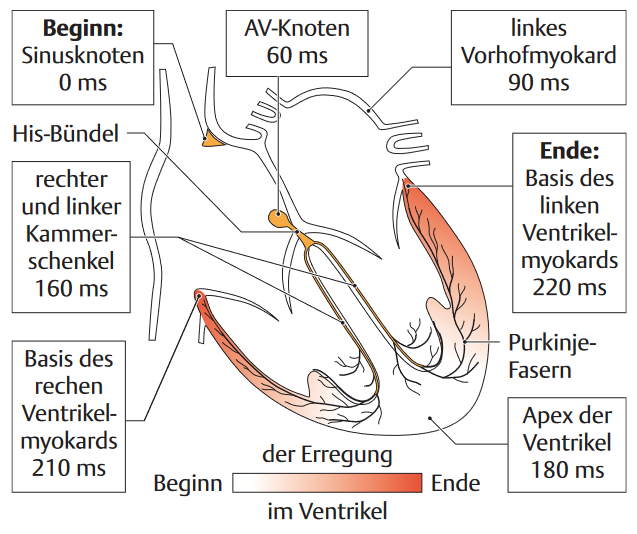
\includegraphics[width=0.80\textwidth]{./Bilder/HerzPhys.png}
\caption[Darstellung des Erregungsleitsystems des Herzens]{Darstellung des Erregungsleitsystems des Herzens. Zu sehen ist die Erregungsausbreitung vom Beginn im Sinusknoten bis zum Ende im Myokard des linken Vorhofes. Zusätzlich angegeben ist die Dauer der Erregungsausbreitung. Entnommen aus \cite{gekle_taschenlehrbuch_2015}.} 
\label{fig:HerzPhys}
\end{figure}  

Vom \gls{AV-Knoten} aus wird die Erregung über das His-Bündel geleitet, über den linken und rechten Tawara-Schenkel am Kammerseptum entlang und in die Purkinje-Fasern hinein. Dieser Teil des Erregungsleitungssystems ist von den Kammermyozyten elektrisch isoliert. Erst die Purkinje-Fasern verzweigen sich ins Kammermyokard und übertragen den Reiz an die Kammermyozyten. Die Zeitspanne von Erregungsbildung im Sinusknoten bis zur vollständigen Erregung der Kammermyozyten beträgt ca. 220 ms. Im Anschluss an die Kammererregung erfolgt die Kammerkontraktion.~\cite{gekle_taschenlehrbuch_2015} 

\section{Funktionsweise der Kardiomyozyten}\label{sec:myozyten}

Wie bereits im vorherigen \hyperref[sec:Erregungsleitsystem]{Abschnitt 2.1} erwähnt, gibt es verschiedene Typen von Kardiomyozyten, welche unterschiedliche Funktionen aufweisen: Erregungsbildung (Sinusknoten), Erregungsweiterleitung (\gls{AV-Knoten} und Purkinjefasern) und Kontraktion (Arbeitsmyokard der Vorhöfe und Kammern). Die Myozyten zur Erregungsbildung und -weiterleitung besitzen außerdem die Fähigkeit, autonom einen Reiz auszulösen, die Myozyten des Arbeitsmyokards nicht. Die Ursache hierfür liegt in den unterschiedlichen Aktionspotentialen der Zelltypen begründet. Ein Aktionspotential ist eine starke Änderung des Membranpotentials einer Zelle und dient der Informationsübertragung. Der Verlauf der Aktionspotentiale (siehe \hyperref[fig:Aktionspotential]{Abb.~2.2}) wird in die Phasen 0 bis 4 eingeteilt, welche im Folgenden näher erläutert werden. \cite{gekle_taschenlehrbuch_2015}

Eine Zelle des Arbeitsmyokards ist in Ruhe bei -90 mV polarisiert (Ruhemembranpotential), dies wird als Phase 4 bezeichnet. Erreicht die Zelle ein elektrischer Reiz, depolarisiert sie auf 0 mV, wobei Natrium-Ionen durch spezifische Kanäle in die Zelle hinein fließen. Dies ist Phase 0 und der Beginn des Aktionspotentials. Während der Depolarisation kommt es zu einem Overshoot, bei welchem die Zelle kurzzeitig bei 20 mV polarisiert ist (Phase 1). \cite{gertsch_ekg_2007}

Auf den Overshoot folgt eine kurze Repolarisation mit anschließendem Plateau im Aktionspotential (Phase 2). Die initiale Repolarisation kommt durch das Fließen von Kalium-Ionen aus der Zelle heraus zustande. Im Laufe dessen öffnen sich Calcium-Ionen-Kanäle, durch die Calcium-Ionen in die Zelle hinein fließen und den Auswärtsstrom der Kalium-Ionen ausgleichen, wodurch das Plateau entsteht. Der Einwärtsstrom der Calcium-Ionen leitet die Kontraktion des Myozyts ein. \cite{gekle_taschenlehrbuch_2015}

In Phase 3 repolarisiert die Zelle durch einen Kalium-Ionen Auswärtsstrom  bis sie sich wieder im Ruhemembranpotential, also in Phase 4, befindet. Die Zelle verbleibt in Phase 4, bis ein erneuter Reiz zur Depolarisation führt. Aufrechterhalten wird das Ruhemembranpotential durch einen kontinuierlichen Austausch von Natrium- und Kalium-Ionen zwischen Intra- und Extrazellulärraum. \cite{gertsch_ekg_2007} 

Übertragen wird ein Reiz von benachbarten Myozyten über sogenannte Gap Junctions, die aus einer Ansammlung unspezifischer Ionenkanäle bestehen, die Connexone genannt werden~\cite{gekle_taschenlehrbuch_2015}.

\begin{figure}[!ht]%
\centering
	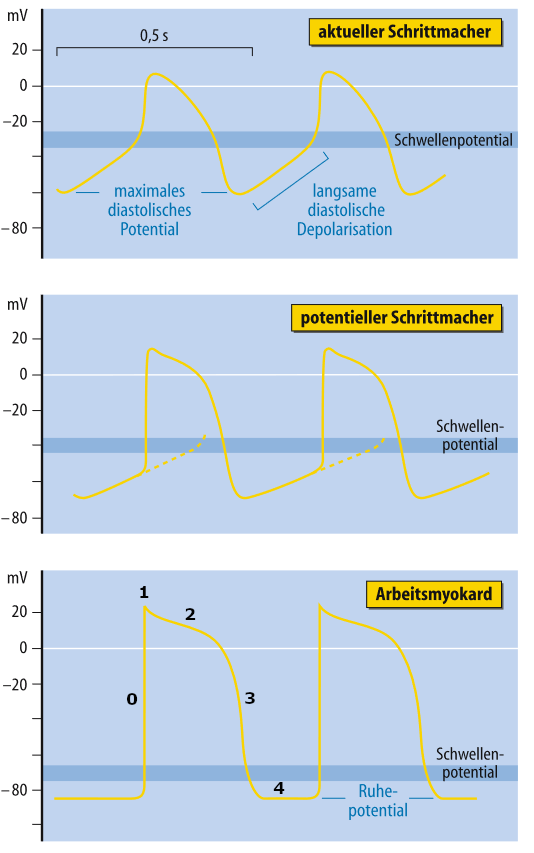
\includegraphics[width=0.80\textwidth]{./Bilder/Aktionspotentiale.png}
\caption[Darstellung von Aktionspotentialen verschiedener Zellen]{Darstellung der Aktionspotentiale einer Sinusknotenzelle (oben), einer Erregungsleitungszelle (mitte) und einer Zelle des Arbeitsmyokards (unten), abgeändert entnommen aus \cite{schmidt_physiologie_2005}. Die Phasen 0 bis 4 des Aktionspotentialverlaufs sind eingetragen.} 
\label{fig:Aktionspotential}
\end{figure}  

Im Gegensatz zu einem Myozyt des Arbeitsmyokards können Sinusknotenmyozyten und Myozyten des Reizleitungsgewebes autonom eine Erregung generieren. Diese Fähigkeit besitzen sie, da sie kein stabiles Ruhemembranpotential haben, sondern in Phase 4 langsam depolarisieren (Spontandepolarisation \cite{schmidt_physiologie_2005}). Diese Depolarisation wird hauptsächlich durch HCN-Kanäle (hyperpolarization activated cyclic nucleotide gated channels) verursacht, durch welche Ionen in die Zelle hineinfließen. Das maximale negative Potential eines Sinusknoten- oder Reizleitungsmyozyts liegt bei -60 mV. Erreicht die Zelle bis zu einem Schwellwert von ca. -40 mV kein Reiz, depolarisiert sie autonom \cite{schmidt_physiologie_2005}. Sinusknoten- und \gls{AV-Knoten}-Myozyten besitzen keine Phase 1 und 2 im Aktionspotential. Bei Myozyten des Sinusknotens wird dieser Schwellwert schneller erreicht, als bei Myozyten des Reizleitungsgewebes, weshalb der Sinusknoten als der primäre Schrittmacher fungiert. Fällt der Sinusknoten aus, kann der \gls{AV-Knoten} als sekundärer Schrittmacher dienen, fällt auch dieser aus, können Teile des Erregungsleitsystems der Ventrikel als tertiärer Schrittmacher einspringen. \cite{gekle_taschenlehrbuch_2015}

Kardiomyozyten sind für einige Zeit nach Beginn der Phase 0 nicht erregbar. Diese Zeit wird als absolute Refraktärphase bezeichnet. Erst wenn das Aktionspotential in Phase 3 wieder bei ca. -40 mV liegt, ist die Zelle wieder durch Reize erregbar. Dies ist die relative Refraktärphase. Um die Zelle in der relativen Refraktärphase zu erregen, ist jedoch ein erheblich stärkerer Reiz notwendig als vom Ruhemembranpotential aus. Da die Refraktärphase länger ist als die Dauer, die zur Depolarisation benötigt wird, wird durch sie eine rückläufige Erregungsausbreitung im Herzen verhindert. \cite{gekle_taschenlehrbuch_2015}


Das Herz muss in der Lage sein, sich dem Bedürfnis des Körpers nach einer erhöhten Sauerstoffversorgung, bspw. beim Sport, anzupassen. Dies wird unter anderem durch eine Erhöhung der Herzfrequenz und der Arbeitslast des Herzens erreicht. Dies ist möglich, da das Herz von Nerven des autonomen Nervensystems innerviert ist. Sympathikus und Vagusnerv haben Einfluss auf die Geschwindigkeit der Spontandepolarisation der Sinusknotenzellen, wodurch eine Frequenzsteigerung (positive Chronotropie) durch Stimulation durch den Sympathikus oder Frequenzsenkung (negative Chronotropie) durch Aktivität des Vagusnervs erzielt wird. Ebenso wird eine Erhöhung der Reizleitungsgeschwindigkeit im \gls{AV-Knoten} (positive Dromotropie) durch Stimulation durch den Sympathikus bzw. Verringerung der Reizleitungsgeschwindigkeit (negative Dromotropie) durch Stimulation durch den Vagusnerv  erzielt. \cite{schmidt_physiologie_2005}

%TODO Refraktärphase mehr? re-entry und vulnerable phase beschreiben

\section{Pathophysiologie von Vorhofflimmern}\label{sec:Vorhofflimmern}

\gls{VHF} ist eine Herzrhythmusstörung, bei der die Vorhoferregung gestört ist und die Vorhöfe somit schnell und unregelmäßig kontrahieren. Durch diese unkoordinierten Vorhofaktionen wird unter Belastung oder bei fortgeschrittenem \gls{VHF} die Füllung der Ventrikel erheblich beeinträchtigt, sodass nicht bei jeder Kammerkontraktion genug Blut ausgestoßen wird. \cite{rizwan_review_2021}

\gls{VHF} wird unterteilt in paroxysmales, persistierendes und permanentes \gls{VHF}, wobei diese Charakterisierung die Dauer der \gls{VHF}-Episode beschreibt. Als paroxysmal wird \gls{VHF} bezeichnet, wenn es unter einer Woche andauert und eigenständig endet (spontane Konversion \cite{gertsch_ekg_2007}). Dauert das \gls{VHF} länger als 7 Tage an, ist eine Kardioversion nötig und das \gls{VHF} wird als persistierend bezeichnet. Persistierendes \gls{VHF} kann in permantentes \gls{VHF} übergehen, wenn die Kardioversion nicht erfolgreich (oder gar nicht) durchgeführt wurde. Im Falle des permanenten \gls{VHF} ist dieses dauerhaft bestehend. \cite{erdmann_klinische_2011} 

Die Entstehung von \gls{VHF} ist ein Zusammenspiel aus Auslösern und Aufrechterhaltungsmechanismus (siehe \hyperref[fig:VHFschematic]{Abb.~2.3}) durch verändertes Gewebe im Vorhof. Die Veränderung des Gewebes zeichnet sich durch Umbau der elektrischen Reizleitungsbahnen sowie strukturelle Veränderungen des Vorhofgewebes aus (auch als Remodelling bezeichnet). \cite{wijesurendra_mechanisms_2019} 

\begin{figure}[!ht]%
\centering
	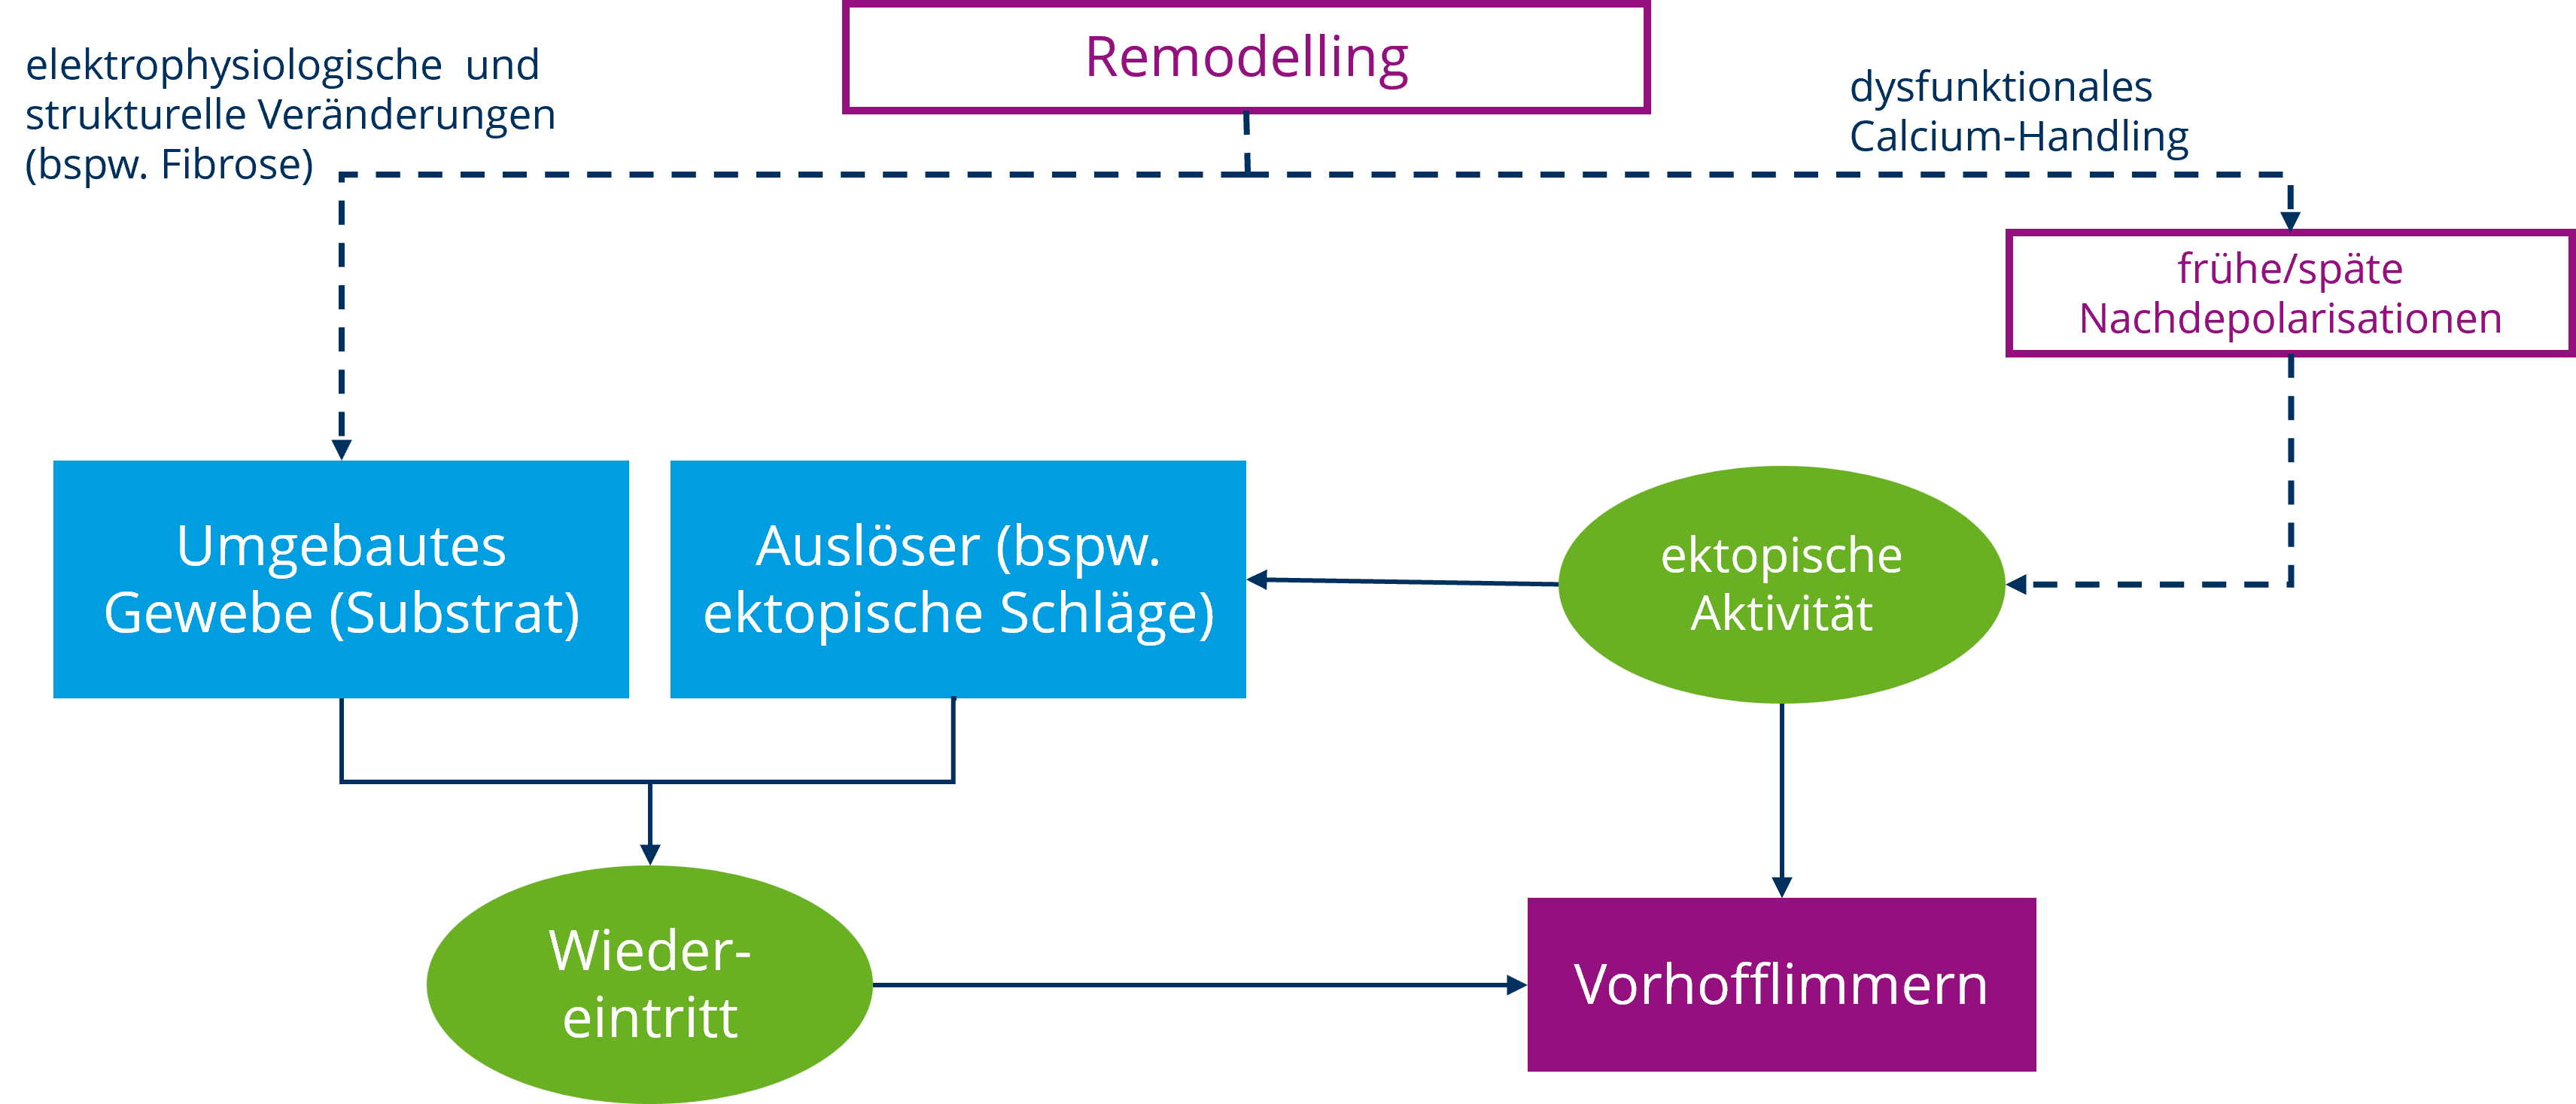
\includegraphics[width=1.0\textwidth]{./Bilder/VHFschematic_new.png}
\caption[Diagramm zur Pathophysiologie von VHF]{Schematische Darstellung von Mechanismen, die zu Vorhofflimmern führen. Eine dysfunktionales Calcium-Handling führt zu frühen oder verspäteten Nachdepolarisationen, welche ektopische Aktivität auslösen. Findet die ektopische Aktivität in hoher Frequenz statt, kann sie Vorhofflimmern aufrecht erhalten. Sie kann auch eine kreisende Erregung verursachen, die Vorhofflimmern aufrecht erhält. Auch ein struktureller und elektrophysiologischer Umbau des Vorhofmyokards kann zu kreisenden Erregungen und damit zu Vorhofflimmern führen. Entommen und übersetzt aus \cite{wijesurendra_mechanisms_2019}.} 
\label{fig:VHFschematic}
\end{figure} 

\subsection{Auslöser von Vorhofflimmern} \label{sec:auslöser}

Paroxysmale \gls{VHF}-Episoden werden durch spontane Depolarisationen von Gewebe mit erhöhter Automatik in oder außerhalb der Vorhöfe (bspw. in der Lungenvene) verursacht. Myozyten, die eine erhöhte Automatik aufweisen, haben ein weniger niedriges maximales negatives Potential, die spontane Phase-4-Depolarisation läuft schneller ab und ein niedrigeres Schwellenpotential ist vorhanden.
Nachdem ein Myozyt mit erhöhter Automatik einen Reiz generiert hat, kann es zu sogenannten frühen Nachdepolarisationen oder verzögerten Nachdepolarisationen kommen. Eine frühe Nachdepolarisation tritt während eines übermäßig verlängerten Aktionspotentials in Phase 3 auf, welches dafür sorgt, dass die deaktivierten Calcium-Kanäle sich erholen und erneut zu einem Calcium-Ionen-Fluss in den Myozyt hinein führen \cite{nattel_molecular_2020}. Eine verzögerte Nachdepolarisation tritt auf, nachdem ein Myozyt bereits zum Ruhemembranpotential zurückgekehrt ist. Sie wird verursacht durch einen Calcium-Überschuss innerhalb der Zelle, der durch Natrium-Calcium-Austauscher zu einem positiven Natrium-Ionen-Fluss in die Zelle hinein führt. Sind die Nachdepolarisationen stark genug, um das Schwellenpotential zu überschreiten, wird ein erneutes Aktionspotential ausgelöst. \cite{khan_identifying_2004}

Die ektopischen Depolarisationen zeichnen sich mit 350 bis 600 Reizen pro Minute durch eine höhere Frequenz als die des Sinusknotens aus \cite{sigg_cardiac_2010}. Hauptausgangspunkt der ektopischen Depolarisationen stellen in 94\% der Fälle die Pulmonalvenen dar \cite{haissaguerre_spontaneous_1998}. Dies liegt daran, dass das Gewebe der Pulmonalvenen andere elektrophysiologische Eigenschaften aufweist, als das Vorhofgewebe \cite{chen_initiation_1999}. Es konnten Myozyten in den Pulmonalvenen nachgewiesen werden, die eine besondere Leitfähigkeit aufweisen, bspw. Schrittmacherzellen und Purkinje-Zellen \cite{perez-lugones_evidence_2003}.
Neben den Pulmonalvenen kann \gls{VHF} auch durch anders verortete ektopische Depolarisationen ausgelöst werden, wie bspw. am Vorhofseptum oder an der posterioren Wand des linken Vorhofs  \cite{santangeli_techniques_2017}. 

Eine Unausgeglichenheit des autonomen Nervensystems kann als Auslöser der ektopischen Aktivität dienen. Hammer et al. \cite{hammer_cardiovascular_2023} zeigen, dass \gls{VHF}-Episoden eine erhöhte Aktivität des Sympathikus vorausgeht, gefolgt von einer erhöhten Aktivität des Vagusnervs.  Eine durch dysfunktionale Sympathikusaktivität erhöhte Ausschüttung von Calcium führt zu einer erhöhten Frequenz von Aktionspotentialen. Eine dysfunktionale Aktivität des Vagusnervs wiederum führt zu einer verkürzten Aktionspotentialdauer und Refraktärperiode. \cite{khan_heart_2019}

\subsection{Aufrechterhaltung von Vorhofflimmern}

\gls{VHF} kann durch die im \hyperref[sec:auslöser]{vorherigen Abschnitt} erwähnten ektopischen Aktivitäten aufrechterhalten werden, wenn diese schnell und andauernd stattfinden. Mit länger anhaltendem \gls{VHF} kommt es zu einem fortschreitendem Umbau des Vorhofmyokards, welcher wiederum \gls{VHF} begünstigt \cite{wijffels_atrial_1995}. Hat sich das Vorhofgewebe bereits umgebaut, kann es durch dieses anfällige Substrat zu einer Reentry-Störung im Vorhof kommen. Substrat, welches empfänglich für Reentry-Störungen ist, zeichnet sich durch strukturelle und elektrophysiologische Veränderungen aus. Es kommt zu kreisenden Erregungen, da einige Leitungsbahnen eine kürzere Refraktärperiode und veränderte Leitgeschwindigkeit aufweisen, sodass die Depolarisationswelle wiederholt auf bereits wieder erregbare Myozyten trifft. Elektrophysiologische Veränderungen können etwa eine Verkürzung der Refraktärperiode, beschleunigte Repolarisation oder eine abnormale Reizleitung durch Veränderungen in den die Myozyten verbindenden Connexonen sein. Die wichtigste strukturelle Veränderung ist eine Dilatation der Vorhöfe und damit einhergehende Fibrose. \cite{wijesurendra_mechanisms_2019}

Es herrscht keine Einigkeit über den Mechanismus, welcher zu langanhaltendem \gls{VHF} führt. Aktuelle Hypothesen bezüglich Reentry-Störungen bei \gls{VHF} beschreiben unabhängige Wavelets, Reentrant Rotors und die Double Layer Hypothese \cite{staerk_atrial_2017}. 

Moe und Abildskov \cite{moe_atrial_1959} haben die Hypothese aufgestellt, dass von einer ektopischen Aktivität eine Depolarisationswelle ausgeht, die sich durch das Vorhofmyokard fortpflanzt und sich aufgrund unterschiedlicher Refraktärperioden der Myozyten in mehrere voneinander unabhängige Wavelets aufspaltet. Diese Wavelets propagieren sich chaotisch weiter durch Gewebe der Vorhöfe, welches bereits erregbar ist, und können sich erneut an refraktärem Gewebe aufspalten oder mit anderen Wavelets zusammenführen.

Unter einem Rotor wird eine um ein nicht erregtes Zentrum kreisende Erregungsausbreitung verstanden. Dieses Zentrum kann sowohl aus nicht erregbarem (bspw. fibrotischem) Gewebe bestehen, aber auch potentiell erregbar sein. Ebenso können Rotoren einen Drift aufweisen und sich somit durch das Vorhofmyokard bewegen. Die Wavelet- und Rotoren-Hypothesen schließen sich nicht gegenseitig aus, da sowohl Wavelets als auch lokalisierte ektopische Depolarisationen einen Rotor auslösen können. \cite{guillem_presence_2016}
 
Die Double Layer Hypothese beschreibt eine longitudinale Dissoziation im Vorhofmyokard, ausgelöst durch parallel zu den Muskelfasern verlaufendes Gewebe mit blockierter Leitfähigkeit. Dies führt zu Bereichen im Vorhofmyokard, die unabhängig voneinander erregbar sind, sodass sich entlang dieser Bereiche Erregungen propagieren können. \cite{allessie_electropathological_2010}


\section{Diagnostik von Vorhofflimmern}\label{sec:DiagVorhofflimmern}

Durch die eingeschränkte Pumpfunktion der Vorhöfe beim \gls{VHF} kann es zu Thrombenbildung in den Vorhöfen kommen. Lösen sich diese und wandern durch den Körper, können sie einen ischämischen Schlaganfall verursachen. Eine frühzeitige Diagnose von \gls{VHF} kann dieses Risiko vermindern. \cite{erdmann_klinische_2011}

Die Symptome von \gls{VHF} sind vielfältig und reichen von Herzrasen über Synkopen und Schmerzen im Brustkorb bis zu Erschöpfung. Da \gls{VHF} jedoch auch asymptomatisch verlaufen kann, ist die Diagnose besonders schwierig. \cite{brundel_atrial_2022}

Das \gls{EKG} ist ein diagnostisches Hilfsmittel, mit welchem Rückschlüsse auf die Reizbildung und -weiterleitung im Herzen gezogen werden können. Es beinhaltet außerdem Informationen über Herzlage, Herzfrequenz und Erregungsrhythmus. \cite{faller_korper_2004}

\subsection{Charakteristika des gesunden Elektrokardiogramms}

%signaltechnische Erfassung und wie das wirklich genau funktioniert

\begin{figure}[!ht]%
\centering
	\includegraphics[width=0.80\textwidth]{./Bilder/ekg.png}
\caption[Musterschlag im EKG]{Darstellung der Intervalle innerhalb eines Musterschlags im Elektrokardiogramm und eines RR-Intervalls, das als Abstand zwischen zwei Kammerdepolarisationen (R-Zacken) definiert ist. Abbildung mit Änderungen angelehnt an  \cite{rizwan_review_2021}.} 
\label{fig:EKG}
\end{figure}  

Die Depolarisation im Herzen führt zu einem elektrischen Feld an der Körperoberfläche. Zwischen verschiedenen Punkten am Körper entstehen so Potentialdifferenzen. Zwischen Elektroden, die auf der Körperoberfläche angebracht werden, wird dadurch eine Spannung erzeugt. Diese Messungen werden als Ableitungen bezeichnet und werden anhand der Elektrodenanordnung unterschieden. Zu den 12 Standardableitungen zählen die 6 Extremitätenableitungen (die bipolaren Ableitungen I, II und III nach Einthoven und die unipolaren Ableitungen aVR, aVL und aVF nach Goldberger), sowie die 6 unipolaren Thoraxableitungen V$_{1}$ bis V$_{6}$ nach Wilson. Die Extremitätenableitungen bilden die elektrischen Reize im Herzen auf die Frontalebene ab, die Thoraxableitungen auf die Horizontalebene, wodurch verschiedene Blickwinkel auf die elektrischen Aktivitäten im Herzen ermöglicht werden.~\cite{faller_korper_2004}

Die Aktivitäten im Herzen lassen sich wie folgt aus dem \gls{EKG} ablesen (siehe \hyperref[fig:EKG]{Abb.~2.4})~\cite{rizwan_review_2021}:
\begin{itemize}
\item \textbf{P-Welle}: Vorhofdepolarisation
\item \textbf{PQ-Strecke}: Atrioventrikuläre Überleitzeit (Erregung durchläuft den AV-Knoten, währenddessen sind die Vorhöfe voll erregt, die Kammern hingegen noch nicht)
\item \textbf{QRS-Komplex}: Kammerdepolarisation
\item \textbf{ST-Strecke}: Unterbrechung der elektrischen Aktivierung der Kammern vor Beginn der Repolarisation (Refraktärzeit, während der ST-Strecke sind die Kammern vollständig erregt)

\item \textbf{T-Welle}: Kammerrepolarisation
\item \textbf{PQ-Intervall}: Beginn der Vorhoferregung bis Beginn der Kammererregung \cite{faller_korper_2004}
\item \textbf{QT-Intervall}: Zeit, die beide Ventrikel zur De- und Repolarisation benötigen, abhängig von der Herzfrequenz \cite{faller_korper_2004}
\item \textbf{RR-Intervall}: Abstand zwischen zwei Kammerdepolarisationen, aus dem RR-Intervall lässt sich die Herzfrequenz berechnen
\end{itemize}

Die Refraktärperiode der Kammern erstreckt sich von der Q-Zacke bis zum Maximum der T-Welle. Anfang der T-Welle beginnt die vulnerable Phase. Währenddessen sind die Kardiomyozyten   
ungleichmäßig refraktär, sodass eine Erregung, die in die vulnerable Phase fällt, eine kreisende Erregung auslösen kann. \cite{schmidt_physiologie_2005}

\subsection{Vorhofflimmern im Elektrokardiogramm}

\gls{VHF} zeichnet sich im \gls{EKG} durch ein unregelmäßiges RR-Intervall aus. Dies kommt zustande, da der \gls{AV-Knoten} nur 20-30\% der chaotischen Vorhofaktionen in die Kammern weiterleitet. Diese Weiterleitung geschieht in chaotischen Intervallen, woraus eine absolute Kammerarrhythmie resultiert, die sich im \gls{EKG} als unregelmäßiges RR-Intervall zeigt (siehe \hyperref[fig:EKG_afib]{Abb.~2.5}). Bei tachykard auftretendem \gls{VHF} kann es zur einer sogenannten Pseudoregularisierung kommen, bei welcher das RR-Intervall regelmäßig erscheint. Auch wenn es zu einem AV-Block kommt und der \gls{AV-Knoten} keine Reize in die Kammern weiterleitet ist das RR-Intervall regelmäßig, da ein untergeordneter Schrittmacher einspringt und einen Ersatzrhythmus erzeugt.

Aufgrund der chaotischen Vorhofaktionen treten anstelle der P-Wellen bei \gls{VHF} Flimmerwellen (F-Wellen) auf, welche in grobe und feine F-Wellen unterschieden werden. Die Sichtbarkeit der F-Wellen ist jedoch ableitungs- und patientenabhängig. Auch bei einer Tachykardie sind die F-Wellen nicht zwingend im \gls{EKG} sichtbar, weshalb das unregelmäßige RR-Intervall als primäres Diagnosekriterium gilt.  \cite{gertsch_ekg_2007}

\begin{figure}[!ht]%
\centering
	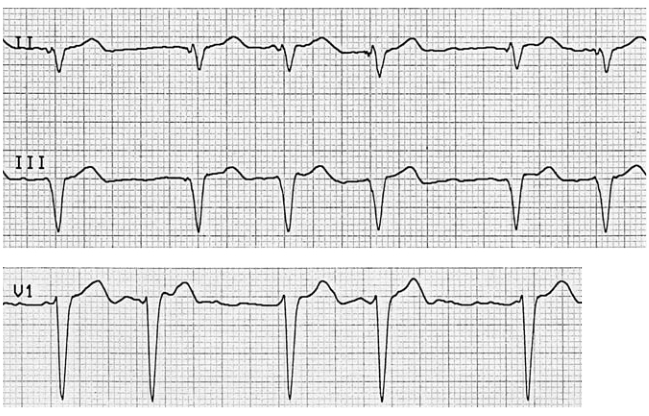
\includegraphics[width=0.80\textwidth]{./Bilder/VHFEKG_fein.png}
\caption[VHF im EKG]{Die Ableitungen II, III und V$_1$ eines Elektrokardiogramms. Zu sehen sind feine Flimmerwellen und eine absolute Kammerarrhythmie. Entnommen aus  \cite{gertsch_ekg_2007}.} 
\label{fig:EKG_afib}
\end{figure} 

%TODO Störungen im EKG? Ableitungsanzahl? \newpage
\chapter{Machine Learning}\label{chap:MachineLearning}

In diesem Kapitel werden in \hyperref[sec:GrundlagenML]{Abschnitt 3.1} die für das weitere Verständnis der Arbeit nötigen Grundlagen zu \gls{ML} und in \hyperref[sec:DL]{Abschnitt 3.2} Grundlagen zu \gls{DL} vermittelt. Metriken zur Bewertung von \gls{ML}-Modellen werden in \hyperref[sec:metriken]{Abschnitt 3.3} eingeführt. Das Prinzip des Domain Shifts wird in \hyperref[sec:shift]{Abschnitt 3.4} erklärt.

\section{Grundlagen des Machine Learnings}\label{sec:GrundlagenML}

Unter \gls{ML} wird ein Prozess verstanden, bei welchem ein Computer aus gegebenen Daten ein statistisches Modell generiert, welches diese Daten abbildet und nach Beendigung der Lernphase gelernte Informationen auf andere Daten verallgemeinern kann. Angewendet wird so ein Modell bspw. für die Klassifikation von Daten in bestimmte Kategorien (bspw. ob ein \gls{EKG}-Abschnitt einen Sinusrhythmus darstellt oder nicht) oder im Falle eines Regressionsproblems für die Vorhersage kontinuierlicher Werte (bspw. die Wahrscheinlichkeit, mit welcher ein Patient \gls{VHF} entwickelt). \cite{nguyen_machine_2018} 

Klassifikation ist der Prozess, ungekennzeichneten Daten automatisch ein Label zuzuweisen. Ein Modell, das dieses Problem löst, heißt Klassifikator. Um ein solches Modell zu erzeugen, nutzt ein Klassifikations-Lernalgorithmus eine Datenmenge mit gelabelten (Supervised Learning) oder ungelabelten (Unsupervised Learning) Beispielen als Eingabe. Die Label bei einer Klassifikationsaufgabe sind Teil einer endlichen Menge von Klassen. Eine Klassifikationsaufgabe mit zwei Klassen nennt sich binäre Klassifikation, mit mehr Klassen wird von einer Multiklassen-Klassifikation gesprochen. \cite{burkov_machine_2019}

Beim Supervised Learning besteht die Datenmenge $\{(x_i, y_i)\}^{N}_{i=1}$ zur Modellerstellung aus gelabelten Beispielen. Ein gelabeltes Beispiel besteht aus einem Merkmalsvektor $x_i$ und einem Label $y_i$. Jede Dimension $j = 1,...,D$ des Merkmalsvektors ist ein einzelnes Merkmal $x^{(j)}$, dass das Beispiel in irgendeiner Weise beschreibt. Bei allen Beispielen in der Datenmenge enthalten die Merkmalsvektoren an derselben Position $j$ dieselbe Art Information (bspw. enthält $x^{(1)}$ das Geschlecht des jeweiligen Patienten). Das Label $y_i$ des Beispiels beschreibt die Ausgabe, die bei Verwendung des Merkmalsvektors als Eingabe in das vom Lernalgorithmus erzeugte Modell erwartet wird. Im Falle eines Klassifikationsalgorithmus ist das Label ein Element einer endlichen Menge $\{1,2,...,C\}$ von Klassen, wobei eine Klasse eine Kategorie beschreibt, der das Beispiel zugeordnet wird.
Die beiden oben genannten Probleme Klassifikation und Regression gehören zum Bereich des Supervised Learning. \cite{burkov_machine_2019} 

Beim Unsupervised Learning besteht die Datenmenge $\{(x_i)\}^{N}_{i=1}$ aus einer Menge ungelabelter Beispiele, wobei ein Beispiel wieder einen Merkmalsvektor $x_i$ enthält, jedoch kein Label \cite{burkov_machine_2019}. Das Ziel des Lernalgorithmus besteht in diesem Fall darin, den Merkmalsvektor als Eingabe zu nehmen und Informationen über die Datenmenge zu erzeugen. Beim sogenannten Clustering teilt das System bspw. die Datenmenge anhand ähnlicher Eigenschaften in verschiedene zusammenhängende Gruppen ein. \cite{nguyen_machine_2018}


\section{Deep Learning}\label{sec:DL}

\gls{DL} ist ein Teilgebiet des \gls{ML} und bezeichnet das Training von tiefen Neuronalen Netzen, also Neuronalen Netzen mit mehr als zwei Schichten zwischen Ein- und Ausgabeschicht. Algorithmen im klassischen \gls{ML} erzeugen sogenannte flache Modelle, indem Parameter direkt anhand der Merkmale der Trainingsbeispiele angepasst werden. Neuronale Netze hingegen erlernen Parameter anhand der Ausgaben der vorhergehenden Schichten. Ein Vorteil von \gls{DL} ist die selbstständige Merkmalsdetektion, sodass im Gegensatz zum klassischen \gls{ML} die Merkmale nicht aufwändig per Hand ausgewählt werden müssen. Jedoch sind \gls{DL}-Modelle im Gegensatz zu klassischen \gls{ML}-Modellen schwer interpretierbar, da die große Anzahl an Schichten es schwierig macht nachzuvollziehen, wie das Modell Entscheidungen trifft.  \cite{burkov_machine_2019}

Goettling et al. \cite{goettling_xecgarch_2024} und Jo et al. \cite{jo_explainable_2021} entwickeln Neuronale Netze mit dem Ziel, deren Entscheidungen nachvollziehbarer zu gestalten.

\subsection{Artificial Neural Network}

Ein \gls{ANN} besteht aus sogenannten künstlichen Neuronen, die in Schichten angeordnet sind. Ein Neuron 

\begin{equation}
\label{Neuron}
O = f(\sum_{j=1}^n x^{(j)} \cdot w^{(j)}+b)
\end{equation}

nimmt einen Merkmalsvektor $x_i = [x^{(1)},..., x^{(n)}]$, multipliziert ihn mit einem Gewichtsvektor $w_i = [w^{(1)},..., w^{(n)}]$, summiert die erhaltenen Werte auf, addiert den Bias $b$, leitet das Ergebnis durch eine Aktivierungsfunktion $f$ und gibt einen einzelnen Wert aus. 

Die Werte der Gewichte (und des Bias) sind die Parameter, die beim Trainieren des Lernalgorithmus erlernt werden. Die Aktivierungsfunktion wird auf die gewichtete Summe aller Eingaben angewandt und fügt dem Neuron die Nichtlinearität hinzu. Sie wird vor dem Training festgelegt, häufig ist es eine der folgenden Funktionen:


\begin{align}
\label{sigmoid}
\text{Sigmoid: } &\quad f(z) = \frac{1}{1+e^{-z}} \\[1em]
\label{tanh}
\text{Tangens hyperbolicus: } &\quad f(z) = \frac{e^z - e^{-z}}{e^z + e^{-z}} \\[1em]
\label{relu}
\text{Rectified Linear Unit: } &\quad f(z) = 
\begin{cases} 
0, & \text{wenn } z < 0 \\ 
z & \text{sonst}
\end{cases}
\\[1em]
\label{softmax}
\text{Softmax: } &\quad f(z) = [f^{(1)},...,f^{(C)}]\text{, wobei } f^{(j)} = \frac{e^{z^{(j)}}}{\sum_{k=1}^C e^{z^{(k)}}}
\end{align}

Die Ausgabe der Softmax-Funktion beschreibt die Wahrscheinlichkeitsverteilung der verschiedenen Klassen C. Die Summe aller Ausgaben $f^{(1)},...,f^{(C)}$ ergibt 1.  Werden mehrere Neuronen zusammengeschaltet erhält man ein \gls{ANN}. In einem \gls{ANN} gibt es eine Eingabeschicht, eine Ausgabeschicht, sowie beliebig viele Schichten zwischen diesen, welche als Hidden Layer bezeichnet werden. Hat ein \gls{ANN} viele Hidden Layer, wird es auch als \gls{DNN} bezeichnet. \cite{burkov_machine_2019}

Es gibt verschiedene Architekturen von \glspl{ANN}. Die simpelste Architektur eines \glspl{ANN} ist das \gls{FFNN} (auch Multilayer Perceptron) \cite{murphy_probabilistic_2022}. In einem \gls{FFNN} existieren keine Schleifen und es gibt einen direkten Weg von Eingabe- zu Ausgabeschicht (siehe \hyperref[fig:ANN]{Abb.~3.1}). Als fully connected bezeichnet man die Schichten, wenn alle Neuronen der Schicht voneinander unabhängig sind, jedes Neuron alle Ausgaben der vorherigen Schicht als Eingaben erhält und seine Ausgaben an alle Neuronen der nachfolgenden Schicht weitergibt. \cite{nielsen_neural_2015}

%\begin{figure}[!ht]%
%\centering
%	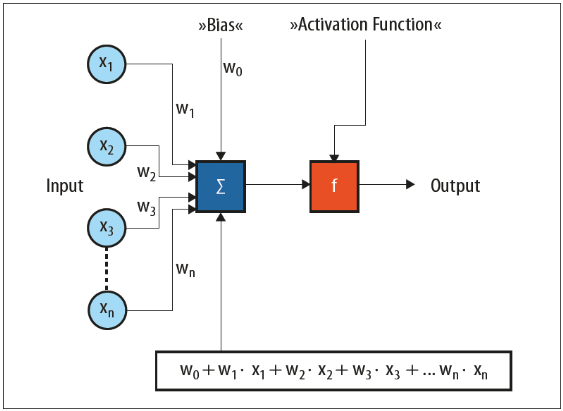
\includegraphics[width=0.80\textwidth]{./Bilder/artificial_neuron.png}
%	\caption[Künstliches Neuron]{Ein künstliches Neuron mit den Eingabewerten %$x_1$ bis $x_n$ und den zugehörigen Gewichten $w_1$ bis $w_n$, sowie dem mit $w_0$ gewichteten Bias, welche aufsummiert und durch die Aktivierungsfunktion $f$ geleitet werden. Ausgegeben wird ein einzelner Wert. Entnommen aus \cite{nguyen_machine_2018}.}
%\label{fig:Neuron}
%\end{figure}

\begin{figure}[!ht]%
\centering
	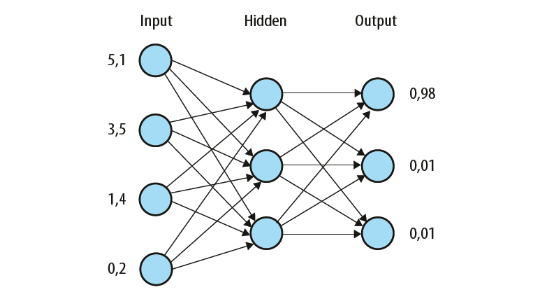
\includegraphics[width=0.80\textwidth]{./Bilder/ANN.png}
	\caption[Feed Forward Neural Network]{Ein Feed Forward Neural Network mit einem fully connected Hidden Layer und beispielhaften Eingangs- und Ausgangswerten. Entnommen aus \cite{nguyen_machine_2018}.}
\label{fig:ANN}
\end{figure}

\subsection{Convolutional Neural Network}

Ein \gls{CNN} ist ein \gls{FFNN}, welches häufig zur Bildverarbeitung eingesetzt wird und gut für Mustererkennung geeignet ist. Es besitzt sogenannte Convolutional Layer, in denen Filter vorhanden sind. Diese Filter sind kleine Matrizen, die jeweils ein anderes Muster erkennen. Dies tun sie, in dem sie stückweise über die Bildmatrix geschoben werden und mit dem Bildausschnitt (Patch) gefaltet werden, den sie überlagern. Je ähnlicher sich Filtermatrix und Patch sind, desto größer ist der Wert, der bei der Convolution erhalten wird. Ein Convolutional Layer in einem \gls{CNN} besteht aus mehreren Filtern, deren Ergebnis jeweils ein Bias-Parameter hinzugefügt wird, bevor die Aktivierungsfunktion angewendet wird. Die Filtermatrix und die Bias-Parameter sind trainierbare Werte in einem \gls{CNN}. Convolutions besitzen eine Schrittweite, die angibt wie weit die Filtermatrix bei jedem Schritt geschoben wird, und ein Padding, welches dem Rand des Bildes hinzugefügt werden kann, damit dieser besser erkennbar ist. Als Aktivierungsfunktion wird üblicherweise die Rectified Linear Unit (ReLu)-Funktion genutzt. Je tiefer der Convolutional Layer ist, desto komplexer werden die Muster, die ein Filter erkennen kann. CNNs besitzen sogenannte Pooling Layer. Ein Pooling Layer folgt üblicherweise auf ein Convolutional Layer. Beim Max-Pooling wird ähnlich wie bei einer Convolution ein Fenster mit einer bestimmten Schrittweite über eine Eingabematrix geschoben, aber anstatt eine Convolution durchzuführen wird der größte Wert im Fenster ausgewählt und ausgegeben. \cite{burkov_machine_2019}

 
Je tiefer ein \gls{DNN} ist, desto schwieriger ist es zu trainieren, da das Degradationsproblem auftritt. Dies bedeutet, dass mit einer zunehmenden Anzahl an Schichten die Genauigkeit eines Modells ab einem bestimmten Punkt gesättigt ist und von da an beginnt zu sinken. Ein Modell mit weniger Schichten hat also eine bessere Leistung als ein Modell mit mehr Schichten, obwohl Letzteres in der Lage sein sollte, komplexere Muster zu erkennen. Ein Grund hierfür kann das \textit{Vanishing Gradient Problem} sein. \textit{Backpropagation} ist ein Algorithmus zur Aktualisierung der Parameterwerte von \gls{ANN}s, mit welchem effizient der Gradient der \gls{ANN}s berechnet werden kann \cite{burkov_machine_2019}. Beim Vanishing Gradient Problem werden während der Backpropagation die Gradienten sehr klein und die Gewichte der vorderen Schichten ändern sich deshalb nicht mehr. 
\glspl{ResNet} lösen das Degradationsproblem, indem sie sogenannte Residualverbindungen (auch Skip oder Shortcut Connections genannt) nutzen, um Schichten zu überspringen. Ein \gls{ResNet} besteht aus mehreren Residual Blocks, welche wiederum aus zwei oder mehr Convolutional Layern bestehen. Die Residual Blocks sind durch Shortcut Connections so verbunden, dass die Eingabe des einen Residual Blocks direkt mit seiner Ausgabe addiert wird und dies als Eingabe für den nächsten Block gilt. Die Shortcut Connections ermöglichen eine effektivere Gradientenweiterleitung während der Backpropagation und ermöglichen das Training tieferer Modelle. \cite{he_deep_2015}

\subsection{Training von Lernalgorithmen}

Das Trainieren eines Lernalgorithmus ist im Grunde das Lösen einer Optimierungsaufgabe. 
Jeder Lernalgorithmus besitzt eine Verlustfunktion (engl. Loss Function), die auch als Fehler bezeichnet wird. Sie ist das Maß dafür, wie stark sich die Ausgabe des Lernalgorithmus von dem tatsächlichen Label unterscheidet. Parameter sind Variablen im erzeugten Modell, deren Werte vom Lernalgorithmus während des Trainings erlernt werden. Sie werden auch als Gewicht und Bias bezeichnet. Gewichte stellen die Stärke der Verbindung zwischen den Neuronen dar und beeinflussen somit, wie stark oder schwach ein Eingangssignal das Neuron aktiviert und wie stark es zur Ausgabe beiträgt. Das Bias ist ebenfalls ein Gewicht, jedoch ist es eine Konstante und ermöglicht es dem Neuron, auch dann aktiviert zu werden, wenn alle Eingaben null sind. 
Die Optimierungsaufgabe besteht darin, die Parameter des Modells iterativ so anzupassen, dass der Wert der Loss Function minimiert wird, sich also die Ausgabe des Lernalgorithmus so gut wie möglich mit dem tatsächlichen Label deckt. \cite{burkov_machine_2019}

Eines der am häufigsten angewandten Verfahren, welches zur Optimierung genutzt wird, ist der Gradientenabstieg (engl. Gradient Descent). Mit ihm kann iterativ das Minimum (oder Maximum) der Loss Function und damit die optimalen Parameterwerte gesucht werden. Eine Iteration wird als Epoche bezeichnet. Der Gradient Descent beginnt mit zufällig ausgewählten Werten für die Parameter. Anschließend wird mit Hilfe der Ableitung die Steigung der Kurve der Loss Function am Punkt der aktuellen Parameterwerte berechnet. Ist die Steigung positiv, werden die Parameterwerte in der nächsten Epoche reduziert, der Punkt wird also im Graphen nach links bewegt. Ist die Steigung negativ, werden die Parameterwerte in der nächsten Epoche erhöht, der Punkt wird also im Graphen nach rechts bewegt. Die Größe dieser Bewegung wird durch die Lernrate (engl. Learning Rate) definiert. Anschließend wird der Vorgang mit den neuen Parameterwerten so oft iteriert, bis ein Abbruchkriterium erfüllt ist. Sobald die Steigung null ist, wurde ein Minimum und somit optimale Parameterwerte gefunden. Allerdings kann es sich dabei um ein lokales Minimum handeln, welches nicht unbedingt bedeutet, dass die absolut optimalen Parameterwerte gefunden wurden. Lokale Minima lassen sich bspw. durch eine dynamische Anpassung der Learning Rate vermeiden. \cite{nguyen_machine_2018}

Der stochastische Gradientenabstieg (engl. Stochastic Gradient Descent) ist eine Version des Gradient Descent, der den Gradienten näherungsweise mit Teilmengen der Trainingsdatenmenge berechnet und so die Berechnung beschleunigt. Beim Training von \gls{ANN}s werden häufig die Varianten \textit{RMSprop} oder \textit{Adam} des Stochastic Gradient Descent genutzt. \cite{burkov_machine_2019}

\subsection{Optimierung der Hyperparameter} 

Hyperparameter werden nicht durch den Lernalgorithmus selbst optimiert und müssen mit einem anderen Verfahren optimiert werden. Wenn die verfügbare Datenmenge groß genug, in der Validierungsmenge jede Klasse in einer ausreichenden Anzahl vertreten und die Anzahl der Hyperparameter sowie deren Wertebereich nicht zu groß ist, kann Rastersuche (engl. Grid Search) genutzt werden. Hierbei werden für jeden Hyperparameter Werte bspw. anhand einer logarithmischen Skala festgelegt. Anschließend werden verschiedene Kombinationen der Hyperparameterwerte zusammengestellt und es wird für jede dieser Kombinationen mit der Trainingsmenge ein Modell erstellt. Anschließend wird die Leistung der Modelle beurteilt. Wenn die optimalen Hyperparameterwerte gefunden wurden, können zusätzlich Werte in der Nähe ausprobiert werden, da sich unter Umständen noch bessere Hyperparameterwerte ergeben können. \cite{burkov_machine_2019}

Bei der Zufallssuche (engl. Random Search) werden im Gegensatz zur Grid Search keine diskreten Wertemengen für die Hyperparameter zusammengestellt, sondern es wird für jeden Hyperparameter eine statistische Verteilung vorgegeben, aus welcher Werte entnommen werden und festgelegt, wie viele Wertekombinationen ausprobiert werden sollen \cite{burkov_machine_2019}. 


\section{Bewertung von Klassifikatoren}\label{sec:metriken}

Die Datenmenge kann in drei Teilmengen aufgeteilt werden: Trainingsmenge, Validierungsmenge und Testmenge. Um den Klassifikator zu validieren, gibt es zwei geläufige Ansätze: Die Holdout-Validierung und die Kreuzvalidierung (engl. Cross Validation). Für die Validierung werden Daten benötigt, die nicht zum Training beigetragen haben. Bei der Holdout-Validierung ist die Trainingsmenge im Idealfall die größte dieser Teilmengen und wird für das Training genutzt. Validierungs- und Testmenge sind sogenannte Holdout-Datenmengen. Sie sind im Idealfall wesentlich kleiner und tragen nicht zum Training bei. Zu beachten ist, dass bei einer insgesamt kleinen Validierungs- und Testmenge die zugrundeliegende Verteilung der Daten unter Umständen nicht vollständig abgebildet wird, sodass die Ergebnisse aus Validierung und Test weniger aussagekräftig sind. Die Validierungsmenge wird verwendet, um den besten Lernalgorithmus auszuwählen und die besten Werte für die Hyperparameter zu ermitteln. Bei der Cross Validation wird die Datenmenge nur in Trainings- und Testmenge aufgeteilt. Die Trainingsmenge wird wiederum in $n$ Mengen aufgeteilt. Anschließend werden $n-1$ Modelle trainiert, wobei jeweils $n-1$ Mengen zum Training und die $n-te$ Menge zur Validierung genutzt wird. In beiden Fällen wird die Testmenge  genutzt, um das finale Modell zu beurteilen, bevor es produktiv eingesetzt wird. \cite{burkov_machine_2019}

Bei dem Erstellen eines Modells können verschiedene Probleme auftreten. Wenn das Modell nicht genug an die Daten angepasst ist, kommt es zur sogenannten Unteranpassung (engl. Underfitting), das Modell hat ein hohes Bias. Das Modell macht also sowohl bei der Vorhersage von Labeln der Trainingsdaten als auch bei denen der Testdaten viele Fehler. Ursache hierfür kann u.A. sein, dass ein zu einfaches Modell gewählt wurde oder die erstellten Merkmale nicht aussagekräftig genug sind. Sagt das Modell die Label der Trainingsdaten sehr gut vorher, aber die der Testdaten nur sehr schlecht, besteht eine Überanpassung (engl. Overfitting), das Modell hat eine hohe Varianz. Dies kann durch ein zu komplex gewähltes Modell auftreten oder dadurch, dass zu viele Merkmale bei nur wenigen Trainingsbeispielen vorliegen. Um die Generalisierbarkeit des Modells zu gewährleisten, sollten die Trainingsdaten eine ausreichende Diversität aufweisen. Dadurch wird vermieden, dass das Modell sich nur an spezifische Eigenheiten der Trainingsdaten anpasst, was ebenfalls zu Overfitting führen kann. Zusätzlich müssen die Testdaten möglichst unabhängig von den Trainingsdaten sein, um eine realistische Einschätzung der Modellleistung auf bisher unbekannten Daten zu ermöglichen.  \cite{burkov_machine_2019}

\subsection{Metriken zur Bewertung der Klassifikationsgüte}
Um festzustellen, ob das Modell Klassen von Daten gut vorhersagen kann, die dem Lernalgorithmus unbekannt sind, gibt es bestimmte Metriken, die in diesem Abschnitt vorgestellt werden.

\subsubsection*{Confusion Matrix}
In einer binären Klassifikationsaufgabe mit den Labeln \textit{positiv} und \textit{negativ} kann man im allgemeinen vier Fälle unterscheiden:
\begin{itemize}
\item \gls{TP}: Anzahl der korrekt als positiv vorhergesagten Label
\item \gls{FP}: Anzahl der fälschlicherweise als positiv vorhergesagten Label
\item \gls{FN}: Anzahl der fälschlicherweise als negativ vorhergesagten Label
\item \gls{TN}: Anzahl der korrekt als negativ vorhergesagten Label
\end{itemize}

Die Matrix in der sie eingetragen werden nennt sich Confusion Matrix (Wahrheitsmatrix).
Ziel ist, die Werte für \gls{TP} und \gls{TN} zu maximieren. Diese Fälle können auch auf Multiklassen-Klassifikationen erweitert werden. \cite{nguyen_machine_2018}

\subsubsection*{Accuracy}

Die Accuracy (Korrektklassifikationsrate) gibt das Verhältnis der Anzahl richtiger Vorhersagen der Labels zur Menge aller untersuchten Beispiele als 
\begin{equation}
\label{eq:accuracy}
Accuracy = \frac{TP+TN}{TP+FP+TN+FN}
\end{equation} \cite{nguyen_machine_2018} an. 


\subsubsection*{Precision-Recall}

Die Precision (Genauigkeit) wird angegeben als \begin{equation}
\label{eq:precision}
Precision = \frac{TP}{TP+FP}
\end{equation} und stellt das Verhältnis der richtigen positiven Vorhersagen zu den positiven Vorhersagen insgesamt dar.  



Recall (auch Sensitivity, Trefferquote oder True-positive-rate) ist das Verhältnis der richtigen positiven Vorhersagen zu den insgesamt in der Datenmenge vorhandenen positiven Beispielen:
\begin{equation}
\label{eq:recall}
Recall = \frac{TP}{TP+FN}
\end{equation}.

Es kann eine Precision-Recall-Kurve generiert werden und anhand der Fläche unter der Kurve (\gls{AUC}) beurteilt werden, wie gut Precision und Recall gleichzeitig sind. Um gute Werte sowohl für Precision als auch für Recall auszuwählen, wird der F1-Score genutzt. Der F1-Score wird entsprechend \begin{equation}
\label{eq:F1}
F1 = \frac{2 \cdot Precision \cdot Recall}{Precision + Recall}
\end{equation} berechnet und ist das harmonische Mittel zwischen Precision und Recall. \cite{nguyen_machine_2018}


\subsubsection*{Specificity}

Die Specificity oder auch True-negative-rate gibt das Verhältnis der richtigen negativen Vorhersagen zu den insgesamt in der Datenmenge vorhandenen negativen Beispielen als
\begin{equation}
\label{eq:specificity}
Specificity = \frac{TN}{TN+FP}
\end{equation}
an.

\subsubsection*{Receiver-Operating-Characteristic-Kurve}

In der \gls{ROC} Kurve wird die Fallout-Rate (False-positive-rate) $fp/(fp+tn)$ gegen den Recall eingetragen. Die Fläche unter der Kurve (\gls{AUC}) ist ein Maß für die Leistung des Modells. \cite{burkov_machine_2019}

\section{Domain Shift}\label{sec:shift}

In der Praxis trifft ein Modell oft auf veränderte Bedingungen: Die Daten, auf denen es trainiert wurde, unterscheiden sich häufig von denen, die es später in der Anwendung sieht. Dieses Phänomen wird Domain Shift genannt \cite{dissanayake_domain_2021}. Ein Domain Shift tritt auf, wenn die Datenverteilung, auf denen ein Modell trainiert wurde (Quelldomäne), unterschiedlich zur Verteilung der Daten, die das Modell in der Praxis sieht (Zieldomäne), ist. Dies führt zu einem Leistungsabfall des Modells. Der Begriff Datenverteilung bezieht sich hierbei auf die statistischen Eigenschaften und Merkmale der Daten insgesamt, nicht nur auf die Häufigkeit der Klassen. \cite{wang_generalizing_2023}

Mathematisch lässt sich eine Domäne $\mathcal{S}$ beschreiben als eine Kombination von Merkmalen $x$ aus einem Eingaberaum $\mathcal{X}$ und Labeln $y$ aus einem Ausgaberaum $\mathcal{Y}$, mit einer zugehörigen Datenverteilung $P_{XY}$. Dies wird als 
\begin{equation}
\mathcal{S} = {(x_i,y_i)^n_{i=1}} \sim P_{XY}
\end{equation}
notiert. $X$ und $Y$ beschreiben die zugehörigen Zufallsvariablen. Die bekanntesten Lösungsansätze für das Domain Shift-Problem sind Transfer Learning, \gls{DAp} und \gls{DG}. \cite{wang_generalizing_2023}

\subsection{Domain Adaptation und Transfer Learning}

Beim Transfer Learning können die Domänen sich in Merkmalsraum, Labelraum und/oder Datenverteilung unterscheiden. \gls{DAp} beschreibt den konkreteren Fall, bei welchem sich die Domänen nur in ihrer Datenverteilung unterscheiden. Da dieser Fall beim Transfer Learning mit inbegriffen ist, kann \gls{DAp} mittels Transfer Learning erreicht werden. \cite{kouw_introduction_2019}

Bei der \gls{DAp} wird ein Modell bspw. mittels Pretraining-Finetuning zuerst auf eine eine Quelldomäne $\mathcal{S}^{src}$ trainiert und anschließend auf eine Zieldomäne $\mathcal{S}^{tar}$ angepasst. Sowohl beim Transfer Learning als auch bei der \gls{DAp} besteht während des Trainings Zugriff auf Daten aus der Zieldomäne $\mathcal{S}^{tar}$. \cite{wang_generalizing_2023} 

\subsection{Domain Generalization}
 
Das Ziel der \gls{DG} ist, ein Modell auf eine oder mehrere unterschiedliche, aber verwandte Domänen $\mathcal{S}^1,...,\mathcal{S}^n$ zu trainieren, sodass es gut auf unbekannte Domänen $\mathcal{S}^{n+1}, \mathcal{S}^{n+2},...$ verallgemeinern kann. Im Gegensatz zur \gls{DAp} besteht während des Trainings kein Zugriff auf Daten aus den Zieldomänen, sodass \gls{DG} zwar ein komplexerer, aber auch ein Ansatz näher an der tatsächlichen Praxis ist. \cite{wang_generalizing_2023}

Methoden für \gls{DG} lassen sich aufteilen in Data Manipulation-basierte Methoden, Representation Learning-basierte Methoden und allgemeine Lernstrategien, die zur \gls{DG} beitragen. Diese Methoden lassen sich kombinieren, um eine noch bessere \gls{DG} zu erreichen. \cite{wang_generalizing_2023}

\subsubsection*{Data Manipulation-basierte Methoden}

Die Kategorie der Data Manipulation-basierten Methoden konzentriert sich auf die Veränderung der Eingabedaten, um die Diversität und Quantität der existierenden Trainingsdaten zu erhöhen, wodurch ein Overfitting reduziert und damit die Fähigkeit des Modells zu Generalisieren erhöht wird. Bei der Data Augmentation werden vorhandene Daten mit Rauschen erweitert, rotiert, zugeschnitten, skaliert oder anderweitig transformiert. Bei der Data Generation werden Daten bspw. mittels eines Generative Adversarial Networks künstlich erzeugt. \cite{wang_generalizing_2023} 

\subsubsection*{Representation Learning-basierte Methoden}

Beim Representation Learning geht es darum, dass Modelle Merkmale erlernen, die die Eingabedaten möglichst gut repräsentieren. Es gibt dazu zwei Lernstrategien, die gut zur \gls{DG} geeignet sind, nämlich Domain Invariant Representation Learning und Feature Disentanglement. 

Beim Feature Disentanglement werden Merkmale in domäneninvariante und domänenspezifische Merkmale getrennt. 
Beim Domain Invariant Representation Learning ist das Ziel, domänenunabhängige Merkmale zu extrahieren. Dies kann bspw. durch Domain Adversarial Learning (siehe \hyperref[sec:DAL]{Abschnitt. 3.4.3}) oder Explicit Feature Alignment erreicht werden. Bei Letzterem wird darauf abgezielt, Merkmalsverteilungen zwischen verschiedenen Domänen explizit anzugleichen. \cite{wang_generalizing_2023} 




\subsubsection*{Allgemeine Lernstrategien zur \gls{DG}}

Es gibt allgemeine \gls{ML} Paradigmen, die sich gut für \gls{DG} eignen. Eine gut geeignete Lernstrategie ist das Ensemble Learning. Hierbei werden mehrere Klassifikatoren trainiert und das Ergebnis bspw. anhand einer Mehrheitsentscheidung aller Modelle bestimmt. Ein Ensemble hat den Vorteil, dass durch die Diversität der Modelle die Gesamtleistung erhöht wird. \cite{wang_generalizing_2023} 

%TODO
 %- Meta Learning
 %- Gradient Operation
 %- Self Supervised Learning
 %- Distributionally Robust Optimization
 
 
Der in dieser Arbeit vorgestellte Ansatz vereint die zwei \gls{DG} Methoden Domain Adversarial Learning und Ensemble Learning.

\subsection{Domain Adversarial Learning}\label{sec:DAL}

Ganin et al. \cite{ganin_domain-adversarial_2016} haben den Ansatz des Domain Adversarial Learnings ursprünglich als Methode zur \gls{DAp} entwickelt. Sie stützen sich hierbei auf die Hypothese, dass die Vorhersagen eines Modells auf Merkmalen getroffen werden müssen, die unabhängig von Quell- und Zieldomäne sind, um den Domain Shift zu überwinden.
Der Ansatz von Ganin et al. nutzt gelabelte Daten aus der Quelldomäne und nicht-gelabelte Daten aus der Zieldomäne und zielt darauf ab, dass Merkmale erlernt werden, die differenzierend für die Hauptklassifikationsaufgabe fungieren, jedoch unempfindlich gegenüber dem Domain Shift sind. 

Ganin et al. führen aus, dass ihr Ansatz mit beinahe jedem \gls{FFNN} funktioniert und das Training mit den Standardmethoden Backpropagation und Gradientenabstieg durchgeführt werden kann.
Die Architektur (\hyperref[fig:DANN_prinzip]{siehe Abb.~3.2}) eines \glspl{DANN} besteht aus einem \textit{Feature Extractor} und einem \textit{Label Predictor}, die zusammen ein Standard-\gls{FFNN} bilden, sowie einem \textit{Domain Classifier}, der mit dem Feature Extractor durch ein \gls{GRL} verbunden ist. Der \gls{GRL} multipliziert den Gradienten während der Backpropagation mit einem konstanten negativen Wert. Die Gradientenumkehr führt dazu, dass das Modell lernt, die Domänen möglichst schlecht zu unterscheiden. \cite{ganin_domain-adversarial_2016}

\begin{figure}[!ht]%
\centering
	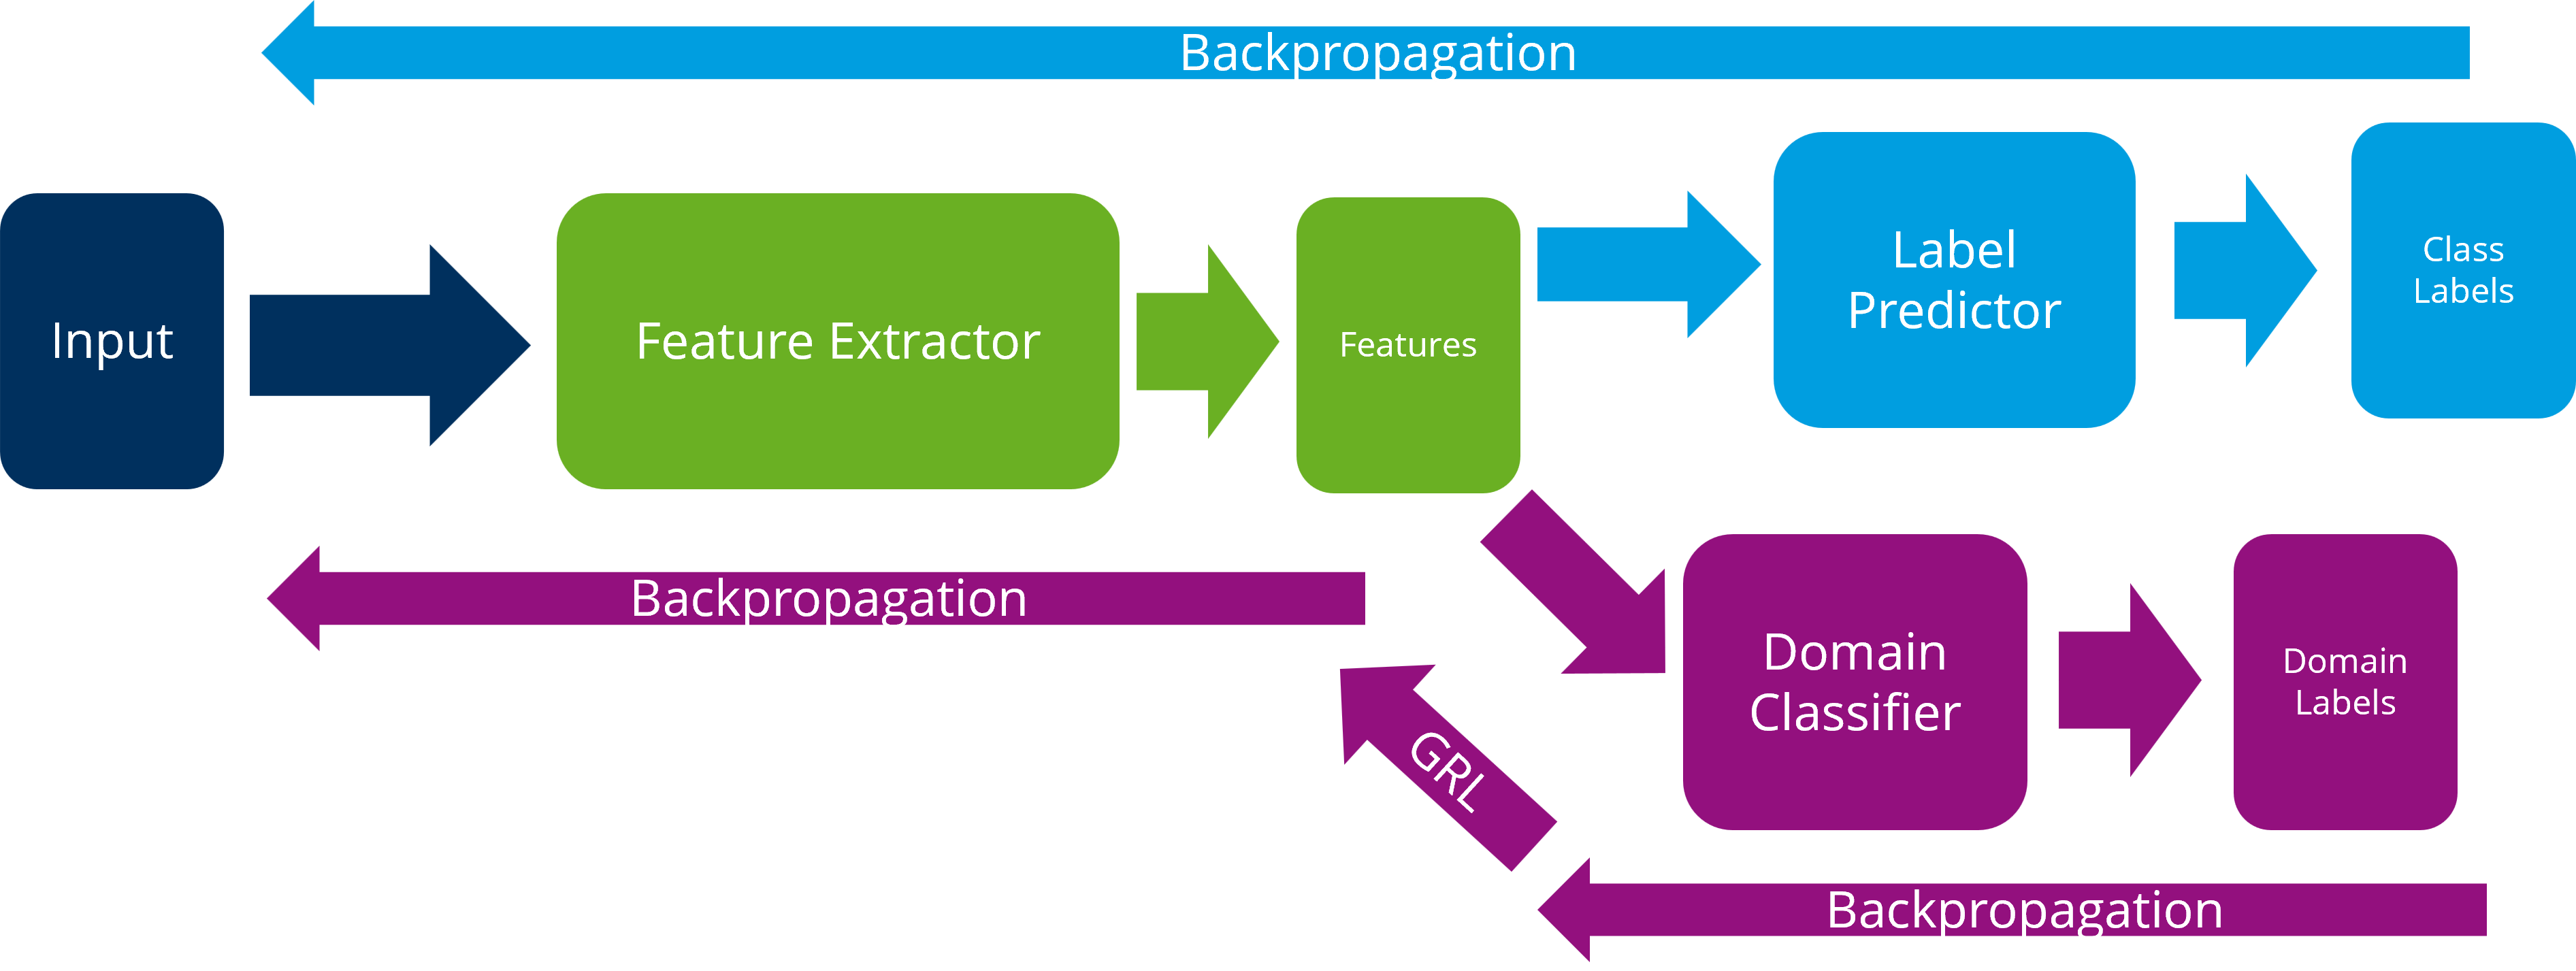
\includegraphics[width=1.0\textwidth]{./Bilder/DANN_aufbau.png}
	\caption[Domain Adversarial Nerual Network Prinzip]{Ein Domain Adversarial Neural Network nach \cite{ganin_domain-adversarial_2016}. Es besteht aus einem Feature Extractor, einem Label Predictor und einem Domain Classifier. Der Gradient des Domain Classifiers wird während der Backpropagation durch den Gradient Reversal Layer (GRL) invertiert. }
\label{fig:DANN_prinzip}
\end{figure}

 \newpage
\chapter{Stand der Technik}\label{chap:sdt}

In diesem Kapitel wird in \hyperref[sec:InceptionTime]{Abschnitt 4.1} zunächst eine Übersicht über aktuelle Ansätze in der Zeitreihenklassifikation gegeben. Anschließend werden in \hyperref[sec:DLEKG]{Abschnitt 4.2} Ansätze zur Klassifikation von \gls{VHF} mittels \gls{DL} zusammengefasst. Zuletzt werden in \hyperref[sec:DGEKG]{Abschnitt 4.3} Vorgehen und die Ergebnisse einer systematischen Literaturrecherche zur \gls{DG} in der \gls{EKG}-Klassifikation präsentiert.

\section{Ansätze zur Zeitreihenklassifikation}\label{sec:InceptionTime}


Da \gls{EKG}-Daten Zeitreihendaten sind, muss für diese Arbeit eine \gls{DNN}-Architektur gewählt werden, die die zeitlichen Abhängigkeiten dieser Daten gut verarbeiten kann.
Fawaz et al. \cite{ismail_fawaz_deep_2019} haben in ihrem Review die gängisten Ansätze zur Zeitreihenklassifikation in einem einheitlichen Rahmen miteinander verglichen. Dazu wurden die gewählten Modelle auf insgesamt 97 uni- und multivariaten Zeitreihendatensätzen trainiert. Die 85 univariaten Zeitreihendatensätze stammen aus dem \textit{\gls{UCR}\slash\gls{UEA} time series archive} \cite{dau_ucr_2019} \cite{bagnall_great_2017}, die 12 multivariaten Datensätze stammen aus \textit{Baydogan's archive} \cite{baydogan_symbolic_2022}, welches 2015 auf der Website heruntergeladen werden konnte, aktuell jedoch nicht. Für univariate Zeitreihendaten, welche in dieser Arbeit als Ein-Kanal-\gls{EKG}s zu finden sind, zeigte beim paarweisen Vergleich von neun \gls{DNN}-Klassifikatoren das \gls{ResNet} die höchste Klassifikationsgüte. Dies ist dargestellt im Critical Difference Diagramm in \hyperref[fig:CritDiffReview]{Abb.~4.1}. Je niedriger der Rang im Diagramm, desto höher ist die durchschnittliche Klassifikationsgüte des Modells. Mit einer Querlinie verbundene Modelle unterscheiden sich statistisch nicht signifikant in ihrer Klassifikationsgüte. Zu sehen ist, dass das \gls{ResNet} einen Score von 2 besitzt und sich somit signifikant von den übrigen Modellen abhebt. Fawaz et al. veröffentlichten das im Rahmen des Reviews entwickelte Framework inklusive der implementierten Klassifikatoren\footnote{https://github.com/hfawaz/dl-4-tsc}. \cite{ismail_fawaz_deep_2019}

Nachträglich wurde von Fawaz et al. eine Website \cite{ali_ismail_fawaz_deep_nodate} erstellt, die eine Übersicht über die Ergebnisse des Vergleichsframeworks der im Review genutzten Klassifkatoren sowie neuerer Ansätze bietet. Ein neuerer Ansatz ist \textit{InceptionTime}, der eine bessere Leistung bezüglich Accuracy erzielt als ein \gls{ResNet}. Zu sehen in \hyperref[fig:CritDiff2]{Abb.~4.2} ist außerdem H-InceptionTime, welches ein hybrider Ansatz ist. Da sich diese Arbeit mit reinen \gls{DL}-Ansätzen beschäftigt, wird H-InceptionTime nicht weiter berücksichtigt.

\begin{figure}[!ht]%
\centering
	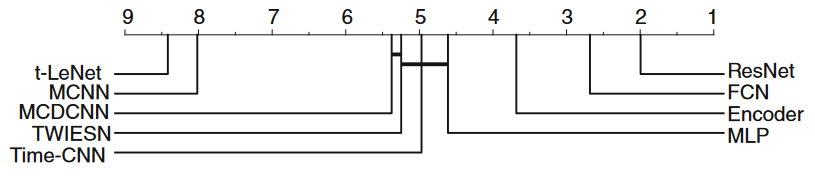
\includegraphics[width=0.80\textwidth]{./Bilder/crit_diff_review.png}
\caption[Critical Difference Diagramm aktueller Deep Neural Networks]{Das Critical Difference Diagramm zeigt die Klassifikationsgüte von neun Deep Neural Networks über das \gls{UCR}\slash\gls{UEA}-Archive im paarweisen Vergleich. Je niedriger der Rang, desto höher ist die durchschnittliche Klassifikationsgüte des Modells. Mit einer Querlinie verbundene Modelle unterscheiden sich statistisch nicht signifikant in ihrer Leistung. Entnommen aus \cite{ismail_fawaz_deep_2019}.} 
\label{fig:CritDiffReview}
\end{figure}  

\begin{figure}[!ht]%
\centering
	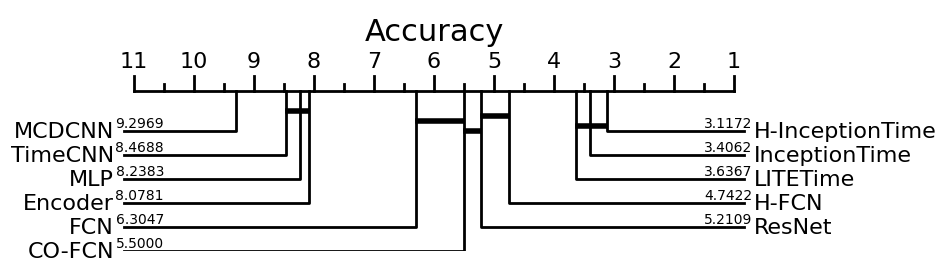
\includegraphics[width=0.80\textwidth]{./Bilder/crit_diff_acc.png}
\caption[Critical Difference Diagramm aktueller Deep Neural Networks und InceptionTime]{Das Critical Difference Diagramm zeigt die Klassifikationsgüte von Deep Neural Networks über das \gls{UCR}\slash\gls{UEA}-Archive im paarweisen Vergleich. Die Rangordnung der Klassifikatoren wurde basierend auf der Accuracy als Metrik erstellt. Je niedriger der Rang, desto höher ist die durchschnittliche Klassifikationsgüte des Modells. Mit einer Querlinie verbundene Modelle unterscheiden sich statistisch nicht signifikant in ihrer Leistung. Entnommen aus \cite{ali_ismail_fawaz_deep_nodate}.} 
\label{fig:CritDiff2}
\end{figure} 

InceptionTime \cite{fawaz_inceptiontime_2020} ist ein Ensemble aus \glspl{CNN} zur Zeitreihenklassifikation, welches auf Incep-tion-v4 basiert, einem \gls{CNN} zur Bildklassifikation. Als Eingabe können sowohl univariate als auch multivariate Zeitreihen dienen.  
Ein einzelner InceptionTime Klassifikator in der Standardkonfiguration ist aufgebaut aus zwei Residual Blocks, welche wiederum aus drei Inception Modulen gebildet werden. Es gibt, wie beim \gls{ResNet}, lineare Shortcut Verbindungen, die den Input des ersten Residual Blocks direkt zum Input des nächsten Residual Blocks hinzufügen. Auf die Residual Blocks folgt ein \gls{GAP} Layer, die den Durchschnitt der entstandenen multivariaten Zeitreihendaten über die gesamte Zeitdimension berechnet. Die letzte Schicht ist ein \gls{FC} Layer mit einer Softmax-Aktivierungsfunktion. Die Anzahl der Neuronen dieser Schicht entspricht der Anzahl der Klassen im Datensatz. In \hyperref[fig:InceptionTime]{Abb.~4.3} ist der Aufbau dargestellt. \cite{fawaz_inceptiontime_2020}

\begin{figure}[!ht]%
\centering
	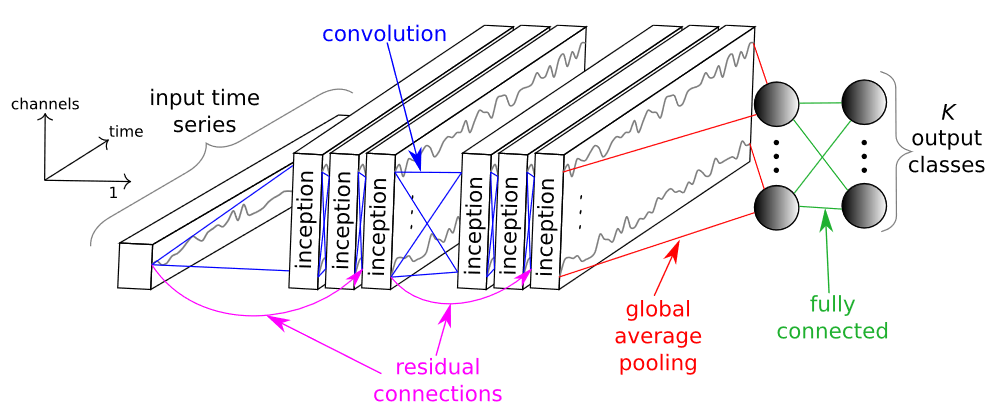
\includegraphics[width=1\textwidth]{./Bilder/InceptionTime.png}
\caption[Darstellung eines InceptionTime Klassifikators]{Darstellung eines einzelnen InceptionTime Klassifikators mit 6 Inception Modulen und einer univariaten Zeitreihe als Eingabe. Entnommen aus \cite{fawaz_inceptiontime_2020}.} 
\label{fig:InceptionTime}
\end{figure}  

In \hyperref[fig:InceptionModul]{Abb.~4.4} ist ein einzelnes Inception Modul dargestellt. Wird eine Zeitreihe der Dimension $M$ in ein Inception Modul eingegeben, so wird sie im ersten Schritt durch ein Bottleneck Layer mit $m$ Filtern mit Wahrnehmungsbereich und Schrittweite 1 auf eine Dimension von $m \ll M$ reduziert. Dies reduziert die Komplexität des Modells und somit auch das Overfitting, während gleichzeitig größere Filter als beim \gls{ResNet} ermöglicht werden. 
Im zweiten Schritt werden Convolutions mit verschieden großen Wahrnehmungsbereichen auf die Ausgabe des Bottleneck Layers angewandt. Parallel zu diesen Convolutions gibt es einen MaxPooling-Pfad, der die maximalen Werte innerhalb eines Fensters zusammenfasst und dadurch die Robustheit des Modells gegenüber Rauschen erhöht. Die Ausgabe der MaxPooling-Operation wird ebenfalls mittels eines Bottleneck Layers in ihrer Dimension reduziert. Die Ausgaben der unabhängigen Convolutions sowie der MaxPooling-Operation werden konkateniert und bilden die Ausgabe des Inception Moduls.
Die Standardkonfiguration eines Inception Moduls besteht aus 3 Filtersets mit jeweils 32 Filtern der Länge $l \in \{10, 20, 40\}$ und MaxPooling. Die Anzahl der Filter pro Schicht entspricht also $32 \times 4=128$. Die Größe des Bottleneck Layers liegt standardmäßig bei $m=32$. \cite{fawaz_inceptiontime_2020} 

Fawaz et al. empfehlen, InceptionTime als Ensemble zu verwenden, da es laut ihnen eine hohe Standardabweichung in der Accuracy zwischen einzelnen InceptionTime Klassifikatoren gibt. Ein InceptionTime Ensemble von Fawaz et al. besteht aus 5 unabhängig voneinander trainierten Modellen. Jedes Modell trägt mit demselben Gewicht zur finalen Vorhersage bei. Die Anzahl der einzelnen Modelle im Ensemble wurde bei 5 festgelegt, da keine signifikante Verbesserung bei mehr als 5 Modellen im Ensemble zu beobachten war.
Das InceptionTime Ensemble wurde mit einem \gls{ResNet} Ensemble der Größe 5 verglichen, da dies das bisher beste \gls{DL}-Ensemble für Zeitreihendaten war. Beide Ensembles wurden mit den 85 Zeitreihendatenbanken des UCR-Archives trainiert und evaluiert. In einem paarweisen Vergleich erzielte das InceptionTime Ensemble bessere Ergebnisse als das \gls{ResNet} Ensemble mit einem Win/Tie/Loss von 54/8/23. \cite{fawaz_inceptiontime_2020}

\begin{figure}[!ht]%
\centering
	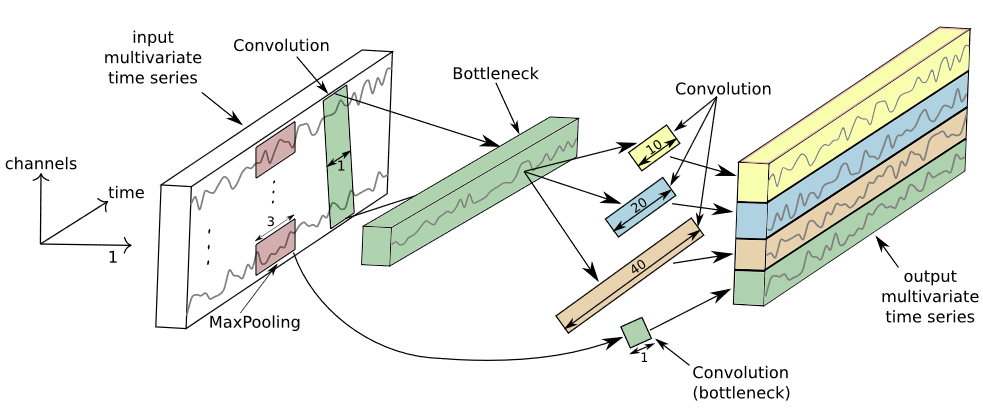
\includegraphics[width=1\textwidth]{./Bilder/InceptionModul.png}
\caption[Darstellung eines einzelnen Inception Moduls]{Darstellung eines einzelnen Inception Moduls mit einem Bottleneck Layer von $m=1$. Entnommen aus \cite{fawaz_inceptiontime_2020}.} 
\label{fig:InceptionModul}
\end{figure} 


%Default Hyperparameter: the default values for InceptionTime are: batch size 64; bottleneck size 32; depth 6; filter length {10,20,40}; and, number of filters 32.
 

\section{Ansätze zur Deep Learning-basierten Vorhofflimmern-Detektion in EKGs}\label{sec:DLEKG}

%full lead ecgs

%reduced lead ecgs
%Hier, das es möglich ist, VHF auf einer reduzierten kanalanzahl zu klassifizieren
%xECG Arch kann man hier auch mit erklären, dann ist das schonmal eingeführt

Es gibt bereits Ansätze zur erfolgreichen \gls{VHF}-Detektion in 12-Kanal-\gls{EKG}s mit Hilfe von \gls{DNN}s \cite{murat_et_al_review_2021}. Auch mit einer reduzierten Kanalanzahl kann \gls{VHF} erfolgreich mittels \gls{DNN}s detektiert werden \cite{murat_et_al_review_2021}. Ein Auszug an Ansätzen zu \gls{VHF}-Detektion sowohl mit voller als auch reduzierter Kanalanzahl ist in \hyperref[tab:DL_AF]{Tab.~4.1} zu sehen. Da in dieser Arbeit 10-Sekunden-\gls{EKG}s verwendet werden, wurden nur Ansätze ausgewählt, welche ebenfalls 10-Sekunden-\gls{EKG}s nutzen. Es werden F1-Scores von bis zu 0,991 mit 12-Kanal-\gls{EKG}s erreicht, sowie von bis zu 0,954 bei Nutzung eines Kanals.

\begin{table}[h!]
\centering
\caption[Deep Learning Ansätze zur VHF-Klassifikation]{Auswahl von Veröffentlichungen die Deep Learning zur Detektion von Vorhofflimmern mit 10-Sekunden-\gls{EKG}s nutzen. Wenn nur eine Ableitung genutzt wurde, wurde die genutzte Ableitung mit angegeben. Bei Lai et al. \cite{lai_non-standardized_2020} handelt es sich um einen Ein-Kanal-\gls{EKG}-Patch mit einer Platzierung, die mit Ableitung II korrespondiert.}
\label{tab:DL_AF}
\begin{tabular}{lllllll}
\hline
\textbf{\makecell{Referenz}} & \textbf{\makecell{Ableitungen}} & \textbf{\makecell{Algorithmus}} & \textbf{\makecell{Spec.}} & \textbf{\makecell{Rec.}} & \textbf{\makecell{Acc.}} & \textbf{\makecell{F1}}\\ \hline
 	\makecell{Attia et al., 2019 \cite{attia_artificial_2019}}	& \makecell{12} 	& \makecell{CNN} 	& \makecell{0,834}	& \makecell{0,823}	& \makecell{0,833} & \makecell{0,454} \\
 	
  	\makecell{Cai et al., 2020 \cite{cai_accurate_2020} }	& \makecell{12} 	& \makecell{DDNN} 	& \makecell{0,994}	& \makecell{0,992}	& \makecell{0,994} & \makecell{0,991}  \\
  	
  	\makecell{Ribeiro et al., 2020 \cite{ribeiro_automatic_2020} }	& \makecell{12} 	& \makecell{ResNet} 	& \makecell{1}	& \makecell{0,769}	& \makecell{-} & \makecell{0,870} \\ 
  	
 	\makecell{Lai et al., 2020 \cite{lai_non-standardized_2020} }	& \makecell{1 (modified II)} 	& \makecell{CNN} 	& \makecell{0,934}	& \makecell{0,931}	& \makecell{0,931} & \makecell{-} \\
 	
 	\makecell{Baalman et al., 2020 \cite{baalman_morphology_2020} }	& \makecell{1 (II)} 	& \makecell{RNN} 	& \makecell{-}	& \makecell{-}	& \makecell{0,960} & \makecell{0,940} \\ 	
 	
  	\makecell{Goettling et al., 2024 \cite{goettling_xecgarch_2024} }	& \makecell{1 (II)} 	& \makecell{CNN} 	& \makecell{0,958}	& \makecell{0,949}	& \makecell{0,953} & \makecell{0,954} \\
  				 		 		
\hline
\end{tabular}
\end{table}

\section{Verwendung von Domain Generalization in der EKG-Klassifikation}\label{sec:DGEKG}


\gls{DG} ist ein relevantes Problem in der \gls{EKG}-Klassifikation, da es eine Vielzahl an möglichen Domain Shifts gibt, jedoch in der Praxis selten bereits ein Testdatensatz während des Trainings vorliegt, um \gls{DAp}-Methoden wie Transfer Learning anzuwenden \cite{hasani_classification_2020}. Im Rahmen dieser Arbeit wurde eine systematische Literaturanalyse zur \gls{DG} in der \gls{EKG}-Klassifikation durchgeführt. Es wurden vier Suchstrings definiert (zu finden in \hyperref[sec:strings]{Anhang A.1}), mit welchen die Literaturdatenbanken \textit{IEEE Xplore}, \textit{PubMed} und \textit{Clarivate Web of Science} durchsucht wurden, resultierend in insgesamt 367 Suchergebnissen. Durch Titel- und Abstrakt-Screening wurden 39 relevante Veröffentlichungen gefunden. Nach dem Volltext-Screening dieser Veröffentlichungen wurden 7 als tatsächlich relevant identifiziert.    

Stammen Aufnahmen aus verschiedenen Krankenhäusern, tritt ein Domain Shift auf, da die \gls{EKG}s unter verschiedenen Bedingungen aufgenommen wurden \cite{hasani_classification_2020}. Ballas \& Diou \cite{ballas_domain_2022} \cite{ballas_towards_2024} beschäftigen sich mit diesem Domain Shift und entwickeln eine \gls{DL}-Architektur, welche auf ein \gls{ResNet}-18 aufsetzt und aus mittleren Convolutional Layern Merkmale extrahiert. Durch diese Extraktion aus mittleren Schichten soll die Verschmelzung von domäneninvarianten mit domänenspezifischen Merkmalen so gering wie möglich gehalten werden.

Hasani et al. \cite{hasani_classification_2020} verwenden als \gls{DG}-Methoden Data Augmentation und Domain Adversarial Learning. Dabei wurden bei der Datenvorverarbeitung zufällig Frequenzen aus den Aufnahmen herausgefiltert oder hinzugefügt, um die statistischen Eigenschaften der Trainingsdaten variabel zu gestalten. Zusätzlich wurden zufällig einzelne Ableitungen durch Nulllinien oder Rauschen ersetzt, Ableitungen vertauscht, Aufnahmen einzelner Ableitungen invertiert, ein Bandpass angewandt oder die Aufnahmen skaliert. Beim Training des Modells wurde ein Domain Adversarial Head mit einem \gls{GRL} und zwei \gls{FC}-Layer mit Dropout hinzugefügt, um die Generalisierung der Modelle über unbekannte Zieldomänen hinweg zu verbessern. Der Feature Extractor des Modells besteht aus zwei parallelen \gls{CNN}s mit unterschiedlich großen Wahrnehmungsbereichen, sodass sowohl grobe als auch feinere Merkmale extrahiert werden können. Auf die \gls{CNN}s folgen zwei \gls{LSTM} Layer, um zeitabhängige Merkmale zu extrahieren. Der Label Predictor besteht aus zwei \gls{FC}-Layern mit Dropout.

Shang et al. \cite{shang_deep_2021} entwickeln ebenfalls ein \gls{DANN} und nutzen als Domain die jeweilige Datenbank aus der die Aufnahmen stammen. Der Feature Extractor des \gls{DANN}s ist ein modifiziertes ResNet mit einem Convolutional Layer mit großen Wahrnehmungsbereich und 8 Residual Blocks. Der Domain Classifier besteht aus einem \gls{GRL} und drei \gls{FC}-Layern mit Dropout, wobei der Label Predictor aus zwei \gls{FC}-Layern ohne Dropout besteht.

Shin et al. \cite{shin_enhancing_2023} nennen ihre Methode zur \gls{DG} \glqq Denoise and Contrast Attention Module\grqq{}, welche auf ein U-Net aufsetzt. Im ersten Schritt werden die Aufnahmen mit Hilfe eines \gls{CNN}s entrauscht. Der Attention-Mechanismus analysiert im Anschluss die Unterschiede in der Morphologie und die zeitlichen Intervalle der Herzschläge, um ventrikuläre Extrasystolen zu detektieren.

Die bisher genannten Ansätze betrachten zwar den Domain Shift zwischen verschiedenen 12-Kanal-\gls{EKG}-Datenbanken, jedoch nicht den Domain Shift, der auftritt, wenn Signale morphologisch verändert sind. Solche Signale treten beim Domain Shift zwischen \gls{EKG}- und \gls{PPG}-Signalen oder zwischen 12-Kanal-\gls{EKG}- und \gls{EKG}-Patch-Signalen mit reduzierter Kanalanzahl auf.

Mit diesem Problem beschäftigen sich Shashikumar et al.~\cite{shashikumar_detection_2018} und Ramesh et al.~\cite{ramesh_atrial_2021}, indem sie Transfer Learning nutzen, um ihre auf \gls{EKG}s trainierten Modelle für \gls{PPG}-Signale anzupassen. Transfer Learning ist jedoch, wie bereits erwähnt, ein Ansatz aus der \gls{DAp} und setzt voraus, dass ein Trainingsdatensatz aus der Zieldomäne vorliegt. Shashikumar et al. \cite{shashikumar_detection_2018} extrahieren zeit-frequenzbezogene Merkmale aus den \gls{EKG}s und \gls{PPG}s und nutzen diese als Merkmale für ihren Klassifikator. 
Ramesh et al. \cite{ramesh_atrial_2021} nutzen nur Merkmale der \gls{HRV} zur \gls{VHF}-Klassifikation, da diese sowohl aus \gls{EKG}- als auch aus \gls{PPG}-Signalen extrahiert werden können. Sie evaluieren die Fähigkeit zur \gls{DG} ihres Modells sowohl mit als auch ohne Transfer Learning. Sowohl Shashikumar et al. \cite{shashikumar_detection_2018} als auch Ramesh et al.\cite{ramesh_atrial_2021} nutzen Ansätze, um auf morphologisch veränderten Signalen als Zieldomäne zu klassifizieren. Jedoch tun sie dies, indem sie Merkmale nutzen, in denen keine Informationen zur Signalmorphologie enthalten sind. In dieser Arbeit wird daher ein Ansatz verfolgt, der die Signalmorphologie berücksichtigt.

Eine Übersicht über verwendete Algorithmen, Methoden zur \gls{DG}, sowie Quell- und Zieldomänen ist in \hyperref[tab:tabelle_related]{Tab.~4.2} zu finden.

\begin{landscape}
\begin{table}[h!]
\centering
\caption[Deep Learning Ansätze zur DG in der EKG-Klassifikation]{Use Cases von Deep Learning Algorithmen zur Klassifikation von Elektrokardiogrammen (EKGs) mit Nutzung von Domain Generalization Methoden. Wenn möglich, wurde der F1-Score angegeben.
HRV: Herzratenvariabilität, PPG: Photoplethysmographie, VES: Ventrikuläre Extrasysolen, VHF: Vorhofflimmern}
\label{tab:tabelle_related}
\begin{tabular}{|l|l|l|l|l|l|l|}
\hline
\textbf{\makecell{Referenz}} & \textbf{\makecell{Algorithmus}} & \textbf{\makecell{Generalization\\Methode}} & \textbf{\makecell{Merkmale}} & \textbf{\makecell{Domänen}} & \textbf{\makecell{Performance\\Quelldomäne}} & \textbf{\makecell{Performance\\Zieldomäne}} \\ \hline

\makecell{Ballas \& Diou,\\ 2022 \cite{ballas_domain_2022}}		& \makecell{ResNet-18}	& \makecell{Feature\\ Disentanglement} & \makecell{Deep Features} & \makecell{12-Kanal-EKG-DBs\\ aus verschiedenen\\ Krankenhäusern} & \makecell{F1 0,94 (VHF)}  & \makecell{F1 0,91 (VHF)} \\ \hline

\makecell{Ballas \& Diou,\\ 2024 \cite{ballas_towards_2024}}		& \makecell{ResNet-18 \\ S-ResNet} & \makecell{Feature\\ Disentanglement} & \makecell{Deep Features} & \makecell{12-Kanal-EKG-DBs\\ aus verschiedenen\\ Krankenhäusern} & \makecell{ResNet-18\\ F1 0,88 (VHF)\\ S-ResNet\\ F1 0,87 (VHF)} & \makecell{ResNet-1\\ F1 0,64 (VHF)\\ S-ResNet\\ F1 0,63 (VHF)} \\ \hline

\makecell{Hasani et al.,\\ 2020 \cite{hasani_classification_2020}} 		& \makecell{CNN-LSTM} & \makecell{Data Augmentation,\\ Domain Adversarial\\ Learning} & \makecell{Alter, Geschlecht,\\ Deep Features} & \makecell{12-Kanal-EKG-DBs\\ aus verschiedenen\\ Krankenhäusern} & \makecell{CinC 2020 score \\ 0,63} & \makecell{CinC 2020 score \\ 0,44} \\ \hline

\makecell{Shang et al.,\\ 2021 \cite{shang_deep_2021} }			& \makecell{SE-ResNet} & \makecell{Domain Adversarial\\ Learning} & \makecell{Alter, Geschlecht,\\ HRV Features,\\ Deep Features} & \makecell{12-Kanal-EKG-DBs\\ aus verschiedenen\\ Krankenhäusern} & \makecell{CinC 2020 score\\ 12-Kanal 0,72\\ 6-Kanal 0,68} & \makecell{CinC 2020 score\\ 12-Kanal 0,44\\ 6-Kanal 0,49} \\ \hline

\makecell{Shin et al.,\\ 2023 \cite{shin_enhancing_2023}}			& \makecell{U-Net +\\ DCAM} & \makecell{Domain Invariant\\ Respresentation Learning\\ with Attention Model} & \makecell{Deep Features} & \makecell{12-Kanal-EKG-DBs\\ aus verschiedenen\\ Krankenhäusern} & \makecell{F1 0,99 (VES)} & \makecell{gemittelt über\\ 6 Zieldomänen\\F1 0,89 (VES)} \\ \hline

\makecell{Shashikumar\\ et al.,\\ 2018 \cite{shashikumar_detection_2018}}	& \makecell{CNN + BRNN +\\ Attention Model} & \makecell{Explicit Feature\\Alignment,\\Transfer Learning} & \makecell{Deep Features,\\ Time Series\\ Covariates,\\ Signal Quality\\ Indices} & \makecell{EKG, PPG} & \makecell{AUC 0,97} & \makecell{AUC 0,94} \\ \hline

\makecell{Ramesh et al.,\\ 2021 \cite{ramesh_atrial_2021}}			& \makecell{CNN} & \makecell{Explicit Feature\\ Alignment,\\ Transfer Learning} & \makecell{HRV Features} & \makecell{EKG, PPG} & \makecell{F1 0,93} & \makecell{Ohne\\ Transfer Learning\\F1 0,72\\Mit\\ Transfer Learning\\F1 0,89} \\ \hline

% &  &  &  &  &  &  \\ \hline
\end{tabular}
\end{table}
\end{landscape} \newpage
\chapter{Methodik}\label{chap:methodik}

In diesem Kapitel werden in \hyperref[sec:daten]{Abschnitt 5.1} zunächst die zum Training und zur Evaluation verwendeten Datensätze und in \hyperref[sec:vorverarbeitung]{Abschnitt 5.2} deren Vorverarbeitung beschrieben. Anschließend wird in \hyperref[sec:architektur]{Abschnitt 5.3} der in dieser Arbeit verwendete Ansatz für ein \gls{DL}-Modell beschrieben. Zuletzt wird in \hyperref[sec:trainingsprozess]{Abschnitt 5.4} auf die Umsetzung dieses Modells genauer eingegangen.

\section{Genutztes Datenmaterial}\label{sec:daten}

In dieser Arbeit wurden vier Datenbanken genutzt: die xECGArch-Datenbank \cite{goettling_xecgarch_2024}, Icentia11k \cite{tan_icentia11k_2021} \cite{tan_icentia11k_2022}, \gls{SHDB-AF} \cite{tsutsui_shdb-af_2024} \cite{tsutsui_shdb-af_2024-1} und eine Datenbank, welche aus dem TIMELY-Datensatz \cite{schmitz_patient-centered_2022} erstellt wurde.

\subsection*{xECGArch-Datenbank}
Für das Training der Modelle wurde die von Goettling et al. \cite{goettling_xecgarch_2024} für  xECGArch erstellte Datenbank verwendet.  
Die xECGArch-Datenbank wurde zusammengesetzt aus den Datenbanken PTB-XL \cite{wagner_ptb-xl_2020} \cite{wagner_ptb-xl_nodate}, Chapman-Shaoxing \cite{zheng_12-lead_2020} \cite{zheng_large_nodate}, Georgia-12-Lead \cite{perez_alday_classification_2020} \cite{perez_alday_classification_nodate} und \gls{CPSC2018} \cite{liu_open_2018}. 
Sie enthält $4~927$ als \gls{VHF} annotierte, sowie $4~927$ als nicht-\gls{VHF} annotierte Aufnahmen. $429$ der nicht-\gls{VHF}-Aufnahmen enthalten einen normalen Sinusrhythmus, Sinus Tachykardie oder Sinus Bradykardie. Die genaue Zusammensetzung der Datenbank aus den Ursprungsdatenbanken kann in \hyperref[tab:Klassenverteilung_xECG]{Tab.~5.1} nachgelesen werden.
Die xECGArch-Datenbank ist aufgeteilt in ein Trainingsset mit $4~420$ \gls{VHF}- und $4~448$ nicht-\gls{VHF}-Aufnahmen, welches für das Training der Modelle in dieser Arbeit genutzt wurde, sowie ein Testset mit $507$ \gls{VHF}- und $479$ nicht-\gls{VHF}-Aufnahmen, welches für die Evaluation in \hyperref[chap:Ergebnisse]{Kapitel 6} genutzt wurde. Die Aufnahmen haben eine Abtastrate von 500~Hz. \cite{goettling_xecgarch_2024}

\begin{table}[h!]
\centering
\caption[Klassenverteilung der xECGArch-Datenbank]{Anzahl und Ursprungsdatenbank der \gls{EKG}-Aufnahmen in der xECGArch-Datenbank. AF steht für Vorhofflimmern, NSR für normalen Sinusrhythmus, ST für Sinustachykardie ohne andere Annotation, SB für Sinusbradykardie ohne andere Annotation und Other umfasst alle anderen Rythmusstörungen. Entnommen aus \cite{goettling_xecgarch_2024}. }
\label{tab:Klassenverteilung_xECG}
\begin{tabular}{lccccc}
\toprule
\textbf{Klasse}       & \multicolumn{5}{c}{\textbf{Datenbank}} \\ 
\cmidrule(lr){2-6}
                     & \textbf{PTB-XL} & \textbf{Georgia} & \textbf{CPSC2018} & \textbf{Chapman-} & \textbf{Total} \\
                     &                 &                  &                   & \textbf{Shaoxing} &                \\ 
\midrule
\textbf{NSR, ST, SB} & 290             & 67               & 12                & 123               & 492            \\
\textbf{OTHER}       & 169             & 2~032            & 1~921             & 313               & 4~435          \\
\textbf{AF}          & 1~497           & 553              & 1~097             & 1~780             & 4~927          \\
\bottomrule
\end{tabular}
\end{table}

%TODO warum balanciert
%TODO 12 Kanal EKGs

\subsection*{Icentia11k}
Da das Ziel dieser Arbeit die Entwicklung eines \gls{DL}-Modells ist, welches robust gegen signalmorphologische Veränderungen bei Aufnahmen mobiler \gls{EKG}-Patches ist, werden zur Evaluation Datenbanken mit Aufnahmen solcher Patches benötigt.
Die Icentia11k-Datenbank~\cite{tan_icentia11k_2021}~\cite{tan_icentia11k_2022} ist zusammengesetzt aus Aufnahmen von 11~000 unterschiedlichen Patienten, welche mit dem CardioSTAT\footnote{https://www.cardiostat.com/} \gls{EKG}-Patch \cite{paquet_adhesive_2022} aufgezeichnet wurden. Dabei handelt es sich um einen Ein-Kanal-Patch, welches mittig auf dem Brustkorb angebracht wird und eine maximale Tragedauer von zwei Wochen hat. Die Aufnahmen der Patienten wurden in ca. einstündige Segmente zerlegt und von Technologen der Icentia inc. (Qu\'ebec, Canada) annotiert. Mögliche Rhythmus-Label sind NSR für normalen Sinusrhythmus, AFib für \gls{VHF} und AFlutter für Vorhofflattern. Einige Abschnitte sind nicht annotiert. Insgesamt gibt es $542~157$ Segmente mit einer Abtastrate von 250~Hz. \cite{tan_icentia11k_2021}


\subsection*{SHDB-AF}

%TODO foto von elektrodenplazierungen bei den drei nicht standard ekg datenbanken

Die \gls{SHDB-AF}~\cite{tsutsui_shdb-af_2024}~\cite{tsutsui_shdb-af_2024-1} ist eine japanische Datenbank, die entwickelt wurde, um die Generalisierfähigkeit von \gls{DL}-Modellen über verschiedene Domain Shifts hinweg zu testen und eignet sich deshalb, um auch das in dieser Arbeit entwickelte Modell zu evaluieren. Die Datenbank setzt sich zusammen aus Aufnahmen von 100 unterschiedlichen Patienten, welche unter paroxysmalem \gls{VHF} leiden. Die Aufnahmen wurden mit dem Holter-Monitor der Fukuda Denshi~Co.,~Ltd.~(Tokyo, Japan) aufgezeichnet und enthalten zwei Kanäle, bei denen es sich um modifizierte CC5- und NASA-Ableitungen handelt. Die \gls{EKG}s sind ca. 24 Stunden lang und wurden mit einer Abtastrate von 125~Hz aufgezeichnet, vor der Veröffentlichung mit einem Bandpass mit den Grenzfrequenzen 0,67 und 100~Hz gefiltert und auf 200~Hz resampelt. Annotiert sind Abschnitte mit \gls{VHF} als AFIB, Vorhofflattern als AFL, Vorhoftachykardie als AT, Vorhofbradykardie als AB und andere supraventrikuläre Tachykardien als PAT oder NOD. Die übrigen Abschnitte erhielten das Label N. \cite{tsutsui_shdb-af_2024}



\subsection*{TIMELY-Datensatz}


%wie viele patienten

Die Daten des TIMELY-Datensatzes wurden im Rahmen des TIMELY Projektes erhoben. 
Ziel des Projekts ist die Entwicklung einer eHealth-Plattform, welche durch künstliche Intelligenz unterstützt wird 
und die Ärzten und Patienten als Hilfsmittel bei der Behandlung von Herzerkrankungen dient. 
Die \gls{EKG}s wurden mit dem net\_ECG-Patch der SEMDATEX GmbH (Berlin, Deutschland)\footnote{https://www.semdatex.com/de/externe-geraete}, welches drei \gls{EKG}-Ableitungen aufnimmt und über dem Herzen platziert wird, aufgezeichnet. Die Aufnahmen haben eine durchschnittliche Dauer von 24 Stunden und eine Abtastrate von 800~Hz. Die Daten sind nicht annotiert, sodass im Rahmen dieser Arbeit ein Datensatz erstellt und annotiert wurde. \cite{schmitz_patient-centered_2022} \cite{noauthor_patient-centered_nodate}


\section{Vorverarbeitung der Datensätze}\label{sec:vorverarbeitung}

Alle Datensätze wurden mit der Python Toolbox \texttt{Neurokit2} \cite{makowski_neurokit2_2021} vorverarbeitet. Gefiltert wurde mit einem Butterworth-Bandpass 4.Ordnung und den Grenzfrequenzen 0.5 und 150 Hz. Diese Grenzfrequenzen wurden ausgewählt, da die diagnostisch relevanten Informationen eines \gls{EKG}s sich innerhalb dieser Frequenzen befinden \cite{kligfield_recommendations_2007}. Genutzt wurde die Implementierung \texttt{butterworth\_ba} von Neurokit2, da diese weniger Randartefakte eingeführt hat als die alternative Implementierung \texttt{butterworth}. Anschließend wurde mit einem Powerline-Filter die Frequenz 50~Hz herausgefiltert. Zuletzt wurden die Daten z-normalisiert.
 
\subsection*{xECGArch-Datenbank}
%test_6lead.json
%train_6lead.json

Das Datenmaterial wurde von der PhysioNet-Website \cite{goldberger_physiobank_2000} zur \textit{PhysioNet/Computing in Cardiology Challenge 2020} \cite{perez_alday_classification_2020} \cite{perez_alday_classification_nodate} heruntergeladen. Genutzt wurden nur Aufnahmen mit mindestens 10 Sekunden Länge. Längere Aufnahmen wurden gekürzt, indem ein 10-Sekunden-Segment aus der Mitte der Aufnahme entnommen wurde. Von den 12 Kanälen der Aufnahmen wurden die Brustwandableitungen nicht verwendet, da sie morphologisch starke Unterschiede zu den Aufnahmen der \gls{EKG}-Patches aufweisen. Die Aufnahmen der meisten \gls{EKG}-Patches enthalten keine Brustwandableitungen, da sie auf Mobilität und einfache Platzierbarkeit ausgelegt sind. Das Einbeziehen der Brustwandableitungen in das Training des \gls{DL}-Modells kann daher kontraproduktiv sein, da das Modell lernen würde, sich auf Signaleigenschaften zu verlassen, die in den mobilen Aufnahmen nicht vorhanden sind. Die übrigen 6 Kanäle I, II, III, aVR, aVL und aVF wurden als einzelne Kanäle für das  Training genutzt.


\subsection*{Icentia11k}

Der Datensatz wurde von der PhysioNet-Website \cite{goldberger_physiobank_2000} heruntergeladen. Zu 363 Segmenten fehlte entweder die Header- oder Annotations-Datei, sodass diese Segmente nicht weiter betrachtet wurden. Um die Menge an Daten zu verringern und die Diversität des Datensatzes dennoch zu erhalten wurde von jedem Patienten ein zufälliges Segment ausgewählt. Aus diesem Segment wurde ein zufälliges 10-Sekunden-Fenster ausgewählt, wobei nicht-annotierte Abschnitte ignoriert wurden. Ist ein gesamtes Segment nicht annotiert, sodass kein 10-Sekun-den-Fenster extrahiert werden kann oder ist das einzige annotierte Intervall kürzer als 10 Sekunden, wird ein anderes Segment ausgewählt. Nach Auswahl der Fenster wurden diese auf 500~Hz mit linearer Interpolation resampelt und anschließend wie zuvor erwähnt gefiltert. Insgesamt gibt es 513 Fenster mit dem Label \gls{VHF} und 10~350 Fenster, die nicht mit \gls{VHF} gelabelt wurden. Die genaue Klassenzusammensetzung lässt sich in \hyperref[tab:Klassenverteilung_Icentia11k]{Tab.~5.2} nachlesen.

\begin{table}[h!]
\centering
\caption[Klassenverteilung im Icentia11k-Datensatz]{Anzahl und Label der 10-Sekunden-Fenster in dem für die Evaluation genutzten Ausschnitt aus der Icentia11k-Datenbank. NSR steht für normalen Sinusrhythmus, AFL für Vorhofflattern und AF für Vorhofflimmern.}
\label{tab:Klassenverteilung_Icentia11k}
\begin{tabular}{ll}
\hline
\textbf{Klasse} & \makecell{\textbf{Anzahl in Icentia11k}} \\ \hline
\textbf{NSR} & \makecell{10~176}   \\
\textbf{AFIB} & \makecell{513} \\
\textbf{AFL} & \makecell{174}  \\ \hline
\end{tabular}
\end{table}

\subsection*{SHDB-AF}

Die \gls{SHDB-AF} wurde von der PhysioNet-Website \cite{goldberger_physiobank_2000} heruntergeladen. Jede Aufnahme wurde auf 500~Hz mit linearer Interpolation resampelt, vollständig in 10-Sekunden-Fenster aufgeteilt und anschließend gefiltert. Insgesamt gibt es 167~288 Fenster mit dem Label \gls{VHF} und 688~090 Fenster, die nicht mit \gls{VHF} gelabelt wurden. Die genaue Klassenzusammensetzung lässt sich in \hyperref[tab:Klassenverteilung_SHDB]{Tab.~5.3} nachlesen. 

\begin{table}[h!]
\centering
\caption[Klassenverteilung in der SHDB-AF-Datenbank]{Anzahl und Label der zur Evaluation genutzten 10-Sekunden-Fenster in der \gls{SHDB-AF}-Datenbank. AFIB bedeutet \gls{VHF}, AFL Vorhofflattern, AT Vorhoftachykardie, AB Vorhofbradykardie und andere supraventrikuläre Tachykardien besitzen die Label PAT oder NOD. Alle übrigen Fenster wurden mit N gelabelt.}
\label{tab:Klassenverteilung_SHDB}
\begin{tabular}{ll}
\hline
\textbf{Klasse} & \makecell{\textbf{Anzahl in SHDB-AF}} \\ \hline
\textbf{N} & \makecell{672~084}   \\
\textbf{NOD} & \makecell{89}   \\
\textbf{PAT} & \makecell{117}   \\
\textbf{AT} & \makecell{2562}   \\
\textbf{AB} & \makecell{366}   \\
\textbf{AFL} & \makecell{12~872} \\
\textbf{AFIB} & \makecell{167~288}  \\ \hline
\end{tabular}
\end{table}

\subsection*{TIMELY-Datensatz} 

Die Rohdaten des TIMELY-Datensatzes wurden am Institut für Biomedizinische Technik der TU Dresden zur Verfügung gestellt. Die Verarbeitung, welche durchgeführt wurde, um aus den Rohdaten einen annotierten Datensatz zu erstellen, wird im Folgenden erklärt.
Es war den Patienten möglich, das EKG-Patch bspw. zum Duschen abzunehmen. Für die Zeitspanne, in der der Patch nicht angebracht war, wurde ein Rechtecksignal und anschließend eine Nullinie aufgezeichnet. Mit Hilfe einer Discard-Mask wurden diese Rechtecksignale, Nullinien, sowie zu niederamplitudige Signale entfernt. Die übrigen Segmente wurden mit Hilfe eines Ensembles aus einem Decision Tree Ensemble von Hammer et al. \cite{hammer_automatic_2021}, xECGArch \cite{goettling_xecgarch_2024} und einem von Ribeiro et al. entwickelten Modell \cite{ribeiro_automatic_2020} klassifiziert. Dafür wurden die Segmente entsprechend den drei Ansätzen vorverarbeitet und in 30- bzw. 10-Sekunden-Fenster zerlegt. Für die 10-Sekunden-Fenster wurden die Aufnahmen von 800~Hz auf 500~Hz mit Nutzung des Mittelwerts als Aggregationsverfahren resamplet. 

Die Patienten sind nicht gleichmäßig im Datensatz vertreten, da alle als \gls{VHF} klassifizierten Fenster aus Aufnahmen von 5 Patienten bestehen. Insgesamt gab es 2~007 als \gls{VHF} klassifizierte Fenster. Um den Datensatz zu erhalten wurden zufällig 2~100 als nicht-\gls{VHF} klassifizierte Fenster ausgewählt. 

Anschließend wurden die automatische Annotation manuell durch zwei Personen unabhängig überprüft. Ein Fenster wurde als \gls{VHF} annotiert, wenn zwei der drei zur Annotation berücksichtigten Parameter \textit{fehlende P-Welle}, \textit{F-Wellen} und \textit{absolute Arrhythmie} mit \textit{ja} beantwortet wurden. Wurden mindestens zwei der Parameter mit \textit{nein} beantwortet, wurde das Fenster mit nicht-\gls{VHF} annotiert. Im Falle von Uneinigkeit der Annotationen wurde das Fenster entfernt. Fenster, bei denen die Ableitung durch extrem starkes Rauschen unbrauchbar war, wurden entfernt. Dadurch entsteht eine leicht unterschiedliche Anzahl an verfügbaren Fenstern pro Ableitung. Die genaue Anzahl lässt sich in \hyperref[tab:Klassenverteilung_Timely]{Tab.~5.3} nachlesen.
Für diese Arbeit wurde der so erhaltene Datensatz aus 10-Sekunden-Fenstern wie zuvor beschrieben mit Neurokit2 gefiltert. 

\begin{table}[h!]
\centering
\caption[Klassenverteilung im TIMELY-Datensatz]{Anzahl und Label der 10-Sekunden-Fenster in dem für die Evaluation genutzten Timely-Datensatz. AF steht für Vorhofflimmern, OTHER für nicht-Vorhofflimmern.}
\label{tab:Klassenverteilung_Timely}
\begin{tabular}{lccc}
\toprule
\textbf{Klasse}       & \multicolumn{3}{c}{\textbf{Anzahl im Timely-Datensatz}} \\ 
\cmidrule(lr){2-4}
                     & \textbf{Ableitung 1} & \textbf{Ableitung 2} & \textbf{Ableitung 3} \\ 
\midrule
\textbf{OTHER}       & 2~303  & 2~284  & 2~245  \\
\textbf{AF}          & 1~660  & 1~660  & 1~661  \\
\bottomrule
\end{tabular}
\end{table}



 
%TODO in den daten vorhandene Distribution Shifts (welches kaptiel? -> grundladen)
% aufnahmegerät
% Patientenherkunft 
% hier wird nur der erste distribution shift angegangen

\section{Modellarchitektur}\label{sec:architektur}

%TODO DANN (warum?)


Das in dieser Arbeit entwickelte Modell soll auf 12-Kanal-\gls{EKG}s trainiert werden, jedoch anschließend in der Lage sein, die \gls{EKG}s von mobilen \gls{EKG}-Patches zu klassifizieren. Da sich die Elektrodenplatzierung mobiler \gls{EKG}-Patches zu der Elektrodenplatzierung beim Goldstandard, dem 12-Kanal-\gls{EKG}, unterscheidet, wird die elektrische Aktivität im Herzen aus einer anderen Perspektive abgebildet. Dies führt dazu, dass die aufgezeichneten \gls{EKG}s signalmorphologische Unterschiede zu den 12-Kanal-\gls{EKG}s enthalten. Es gibt also in der Signalmorpholgie einen Domain Shift von der Quelldomäne, dem 12-Kanal-\gls{EKG}, hin zur Zieldomäne, den Aufnahmen der mobilen \gls{EKG}-Patches.

Um diesem Domain Shift entgegenzuwirken, werden zwei Methoden aus der \gls{DG} angewandt: Domain Adversarial Learning und Ensemble Learning.

\subsection*{Domain Adversarial Neural Network}

Die Architektur des \gls{DANN}s ist in \hyperref[fig:DANN]{Abb.~5.1} dargestellt. Als Eingabe dienen 1-Kanal-\gls{EKG}s mit den Domain Labels I, II, III, aVR, aVL und aVF und den Zielklassen Labels \gls{VHF} und nicht-\gls{VHF}. Als Feature Extractor des \gls{DANN}s wurde ein einzelner InceptionTime Klassifikator im klassischen InceptionTime Design (siehe \hyperref[sec:InceptionTime]{Kapitel 4.1}) gewählt.

  In jedem Inception Modul sind somit 3 Filtersets mit jeweils 32 Filtern mit den unterschiedlichen Filtergrößen $l \in \{10, 20, 40\}$ enthalten. Filtergrößen mit geringerem Wahrnehmungsbereich dienen zur Erkennung feinerer Muster im \gls{EKG} wie P-Welle und F-Wellen, wobei sich Filter mit größerem Wahrnehmungsbereich besser zur Erkennung von längerfristigen Merkmalen wie einer absoluten Arrhythmie eignen. %TODO zitat?
Die Anzahl der Inception Module wurde als Hyperparameter in der Grid Search ermittelt. 
 
An den \gls{GAP}-Layer des Feature Extractors wurden angelehnt an die Modelle von Ganin~et~al.~\cite{ganin_domain-adversarial_2016} ein Domain Classifier und ein Label Predictor angebracht. Der Domain Classifier besteht aus zwei \gls{FC}-Layern mit \gls{ReLU} als Aktivierungsfunktion und einem \gls{FC}-Layer mit 6 Neuronen als Ausgabeschicht mit einer Softmax-Aktivierungsfunktion. Der Label Predictor besteht ebenso aus zwei \gls{FC}-Layern mit einer \gls{ReLU}-Aktivierungsfunktion. Die Ausgabeschicht ist ein \gls{FC}-Layer mit 2 Neuronen und einer Softmax-Aktivierungsfunktion.

\begin{figure}[!ht]%
\centering
	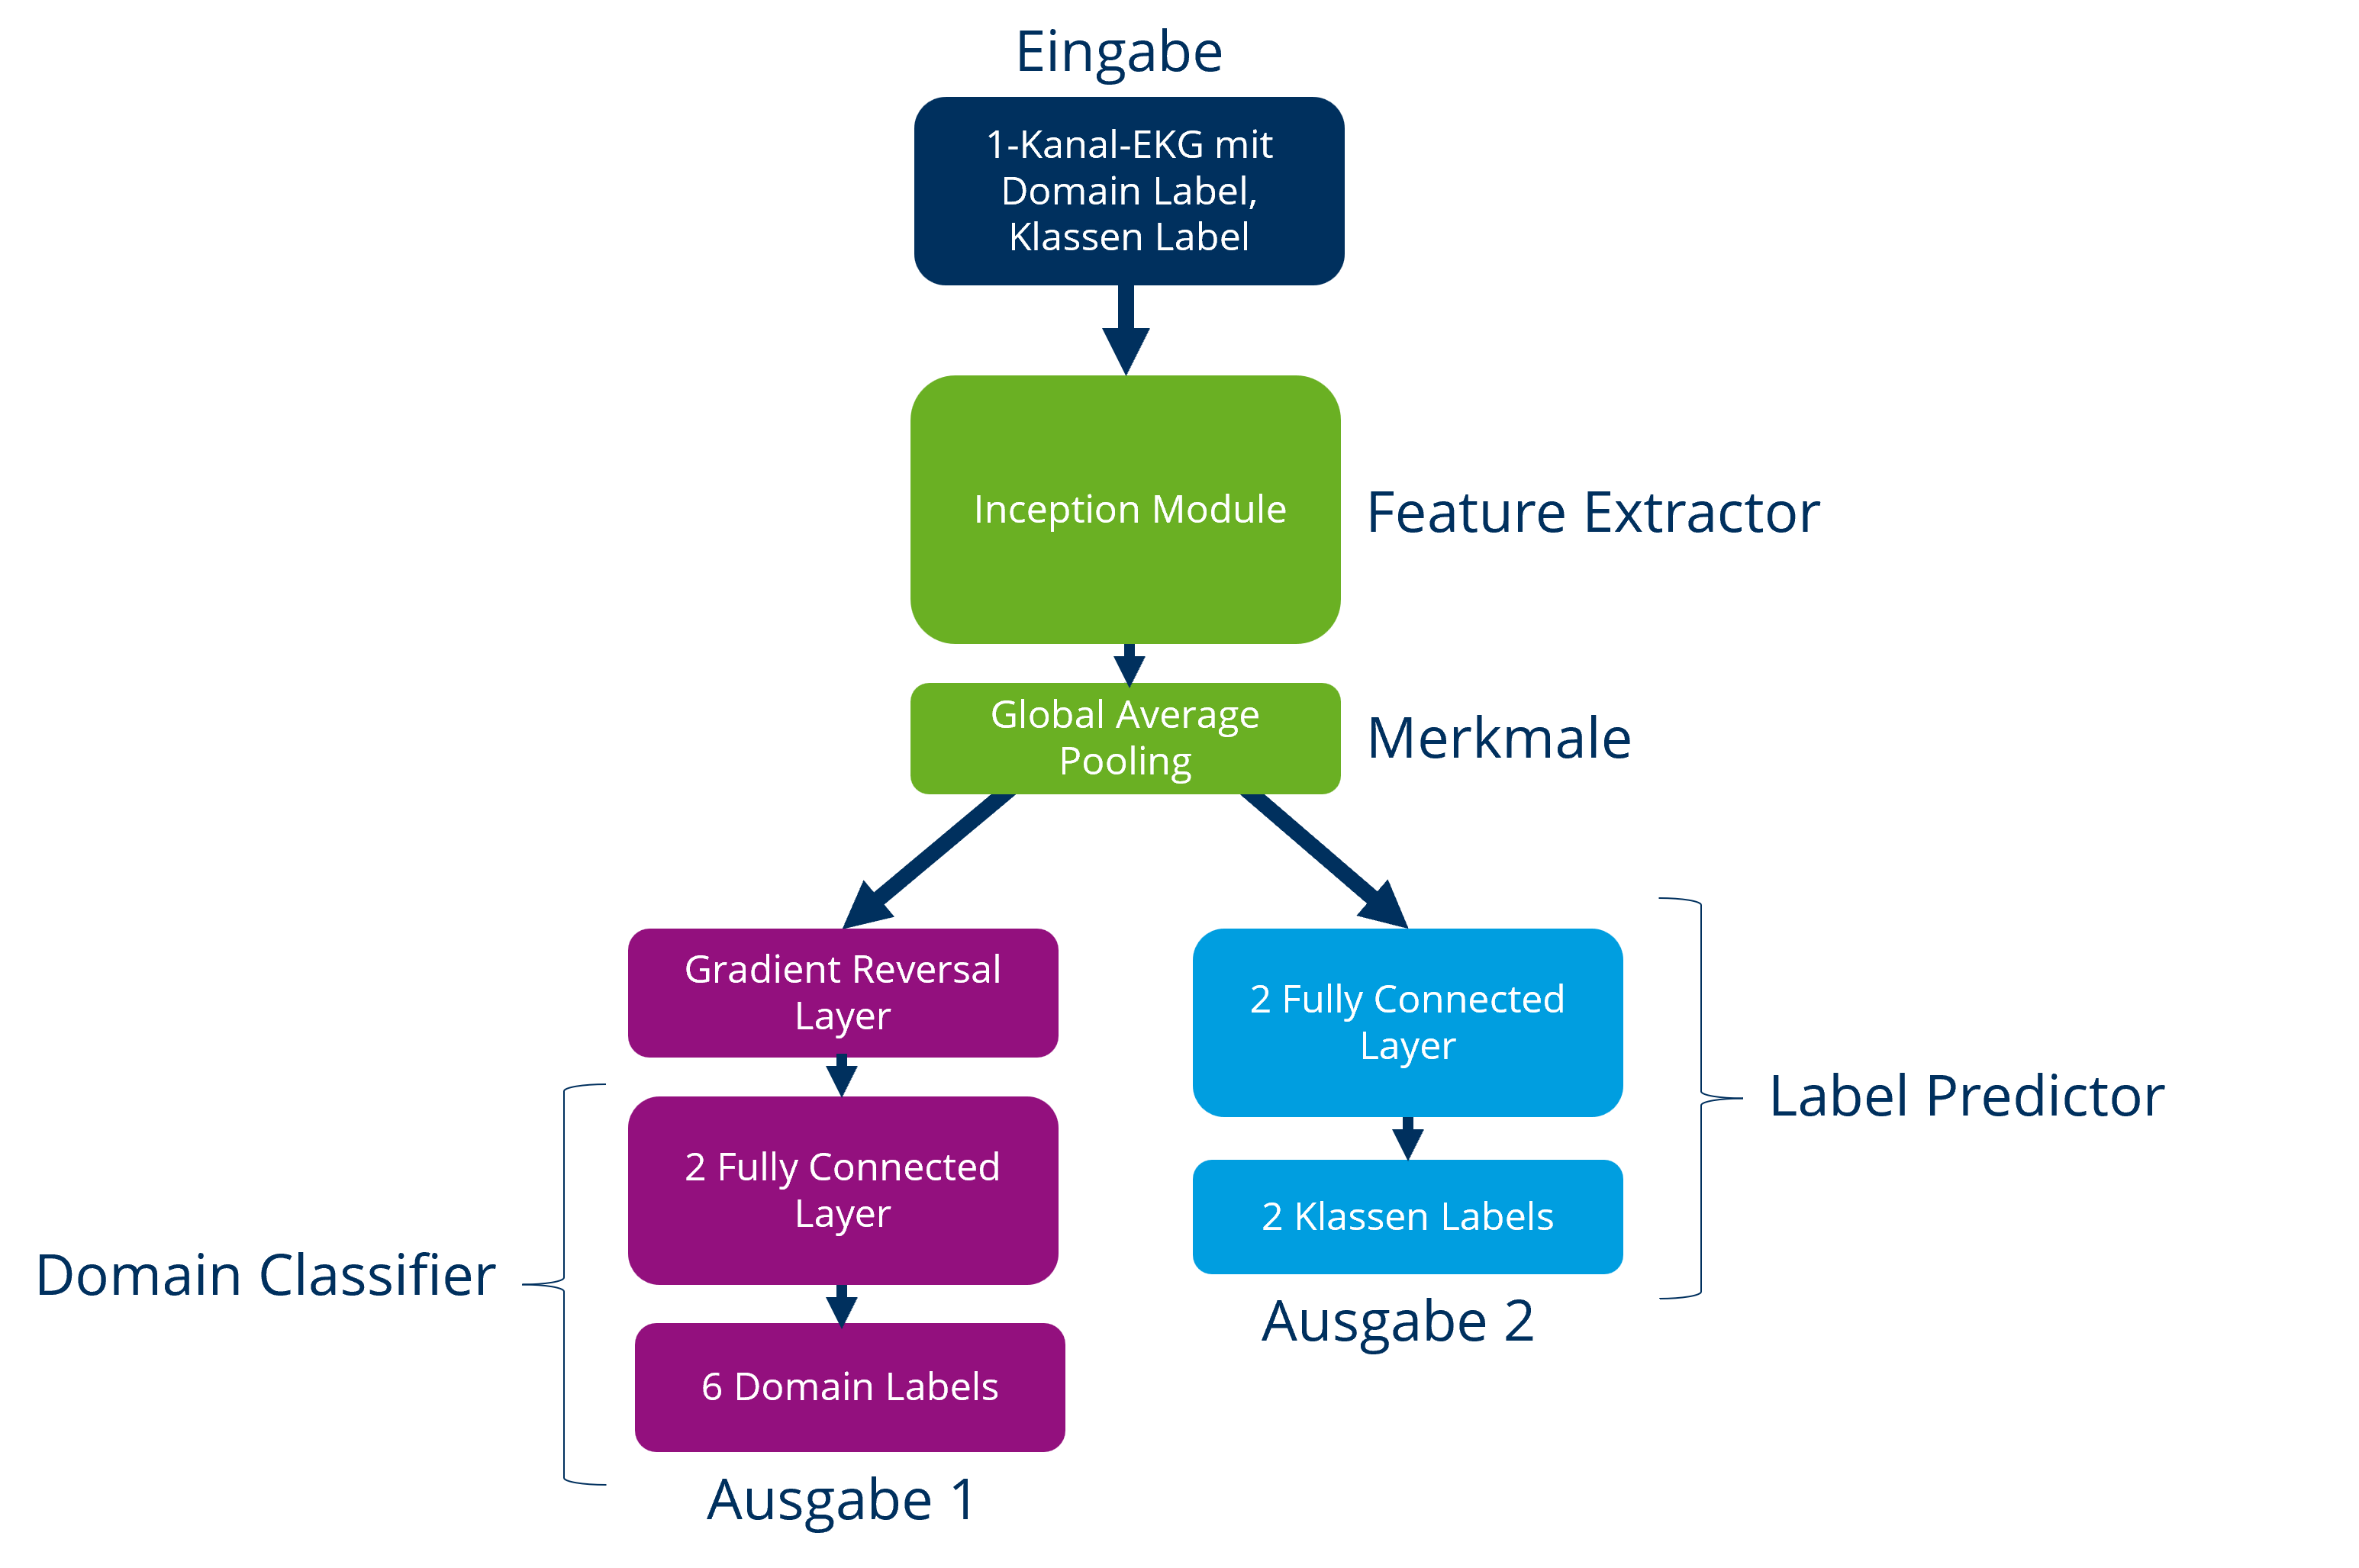
\includegraphics[width=1\textwidth]{./Bilder/DANN_architektur.png}
\caption[DANN Architektur]{Architektur des \gls{DANN}s. Als Eingabe dienen 1-Kanal-\gls{EKG}s. Als Feature Extractor dient InceptionTime. Für den Domain Classifier wird an den \gls{GAP}-Layer der \gls{GRL} angeschlossen, worauf zwei \gls{FC}-Layer folgen. Die Ausgabeschicht des Domain Classifiers besitzt 6 Neuronen für die 6 Domänen. Der Label Predictor besitzt 2 \gls{FC}-Layer angeschlossen an den \gls{GAP}-Layer und 2 Neuronen als Ausgabeschicht für die zwei Zielklassen \gls{VHF} und nicht-\gls{VHF}.} 
\label{fig:DANN}
\end{figure} 

\subsection*{DANN mit Direktausgabe der Merkmale}

Zur Untersuchung des Einflusses der Feature-Transformation, die in den \gls{FC}-Layern stattfindet, auf die Generalisierungsfähigkeit des Modells wird ein \gls{DANN} ohne \gls{FC}-Layer zwischen \gls{GAP}-Layer und Ausgabeschicht im Label Predictor trainiert. Dadurch werden die Merkmale aus dem Feature Extractor ohne Zwischenrepräsentationen direkt ausgegeben. Diese Version des \gls{DANN}s wird im weiteren Verlauf der Arbeit als DANNdirect bezeichnet und ist in \hyperref[fig:DANNdirect]{Abb.~5.2} dargestellt.

\begin{figure}[!ht]%
\centering
	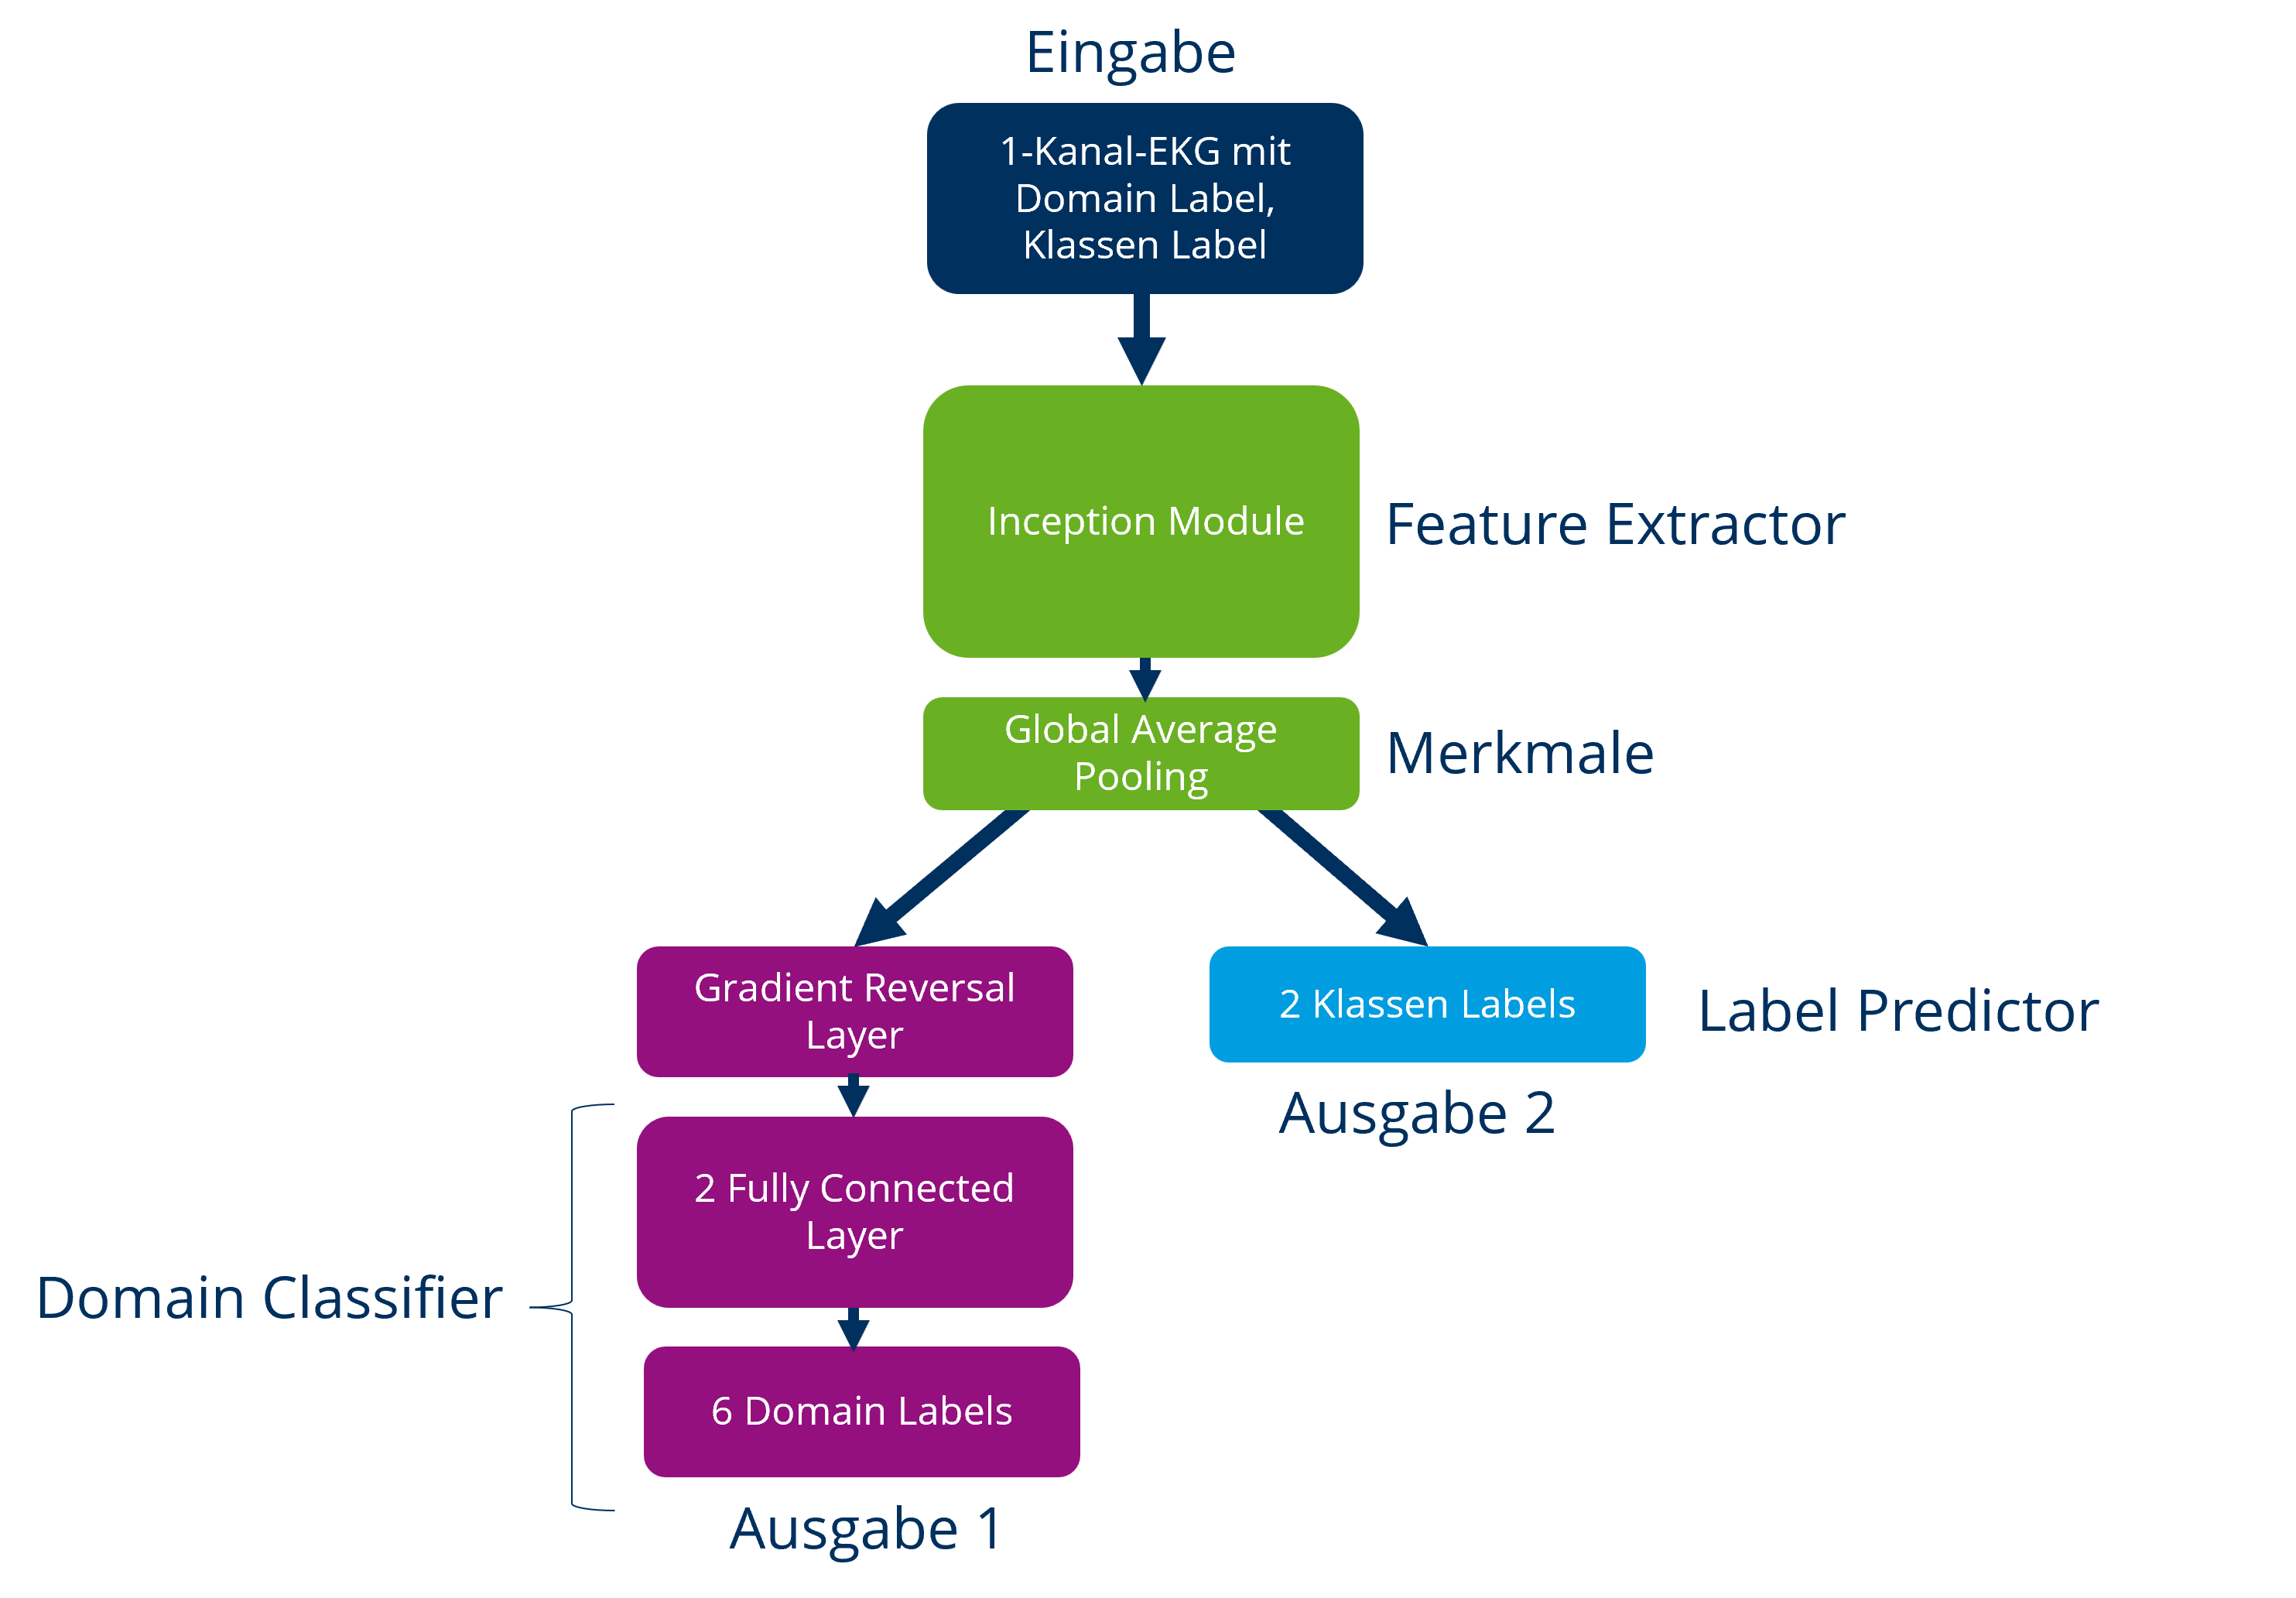
\includegraphics[width=1\textwidth]{./Bilder/DANNdirect_architektur.png}
\caption[DANNdirect Architektur]{Architektur des \gls{DANN}direct Modells. Als Eingabe dienen 1-Kanal-\gls{EKG}s. Als Feature Extractor dient InceptionTime. Für den Domain Classifier wird an den \gls{GAP}-Schicht den \gls{GRL} angeschlossen, worauf zwei \gls{FC}-Layer folgen. Die Ausgabeschicht des Domain Classifiers besitzt 6 Neuronen für die 6 Domänen. Der Label Predictor besitzt 2 Neuronen als Ausgabeschicht für die zwei Zielklassen \gls{VHF} und nicht-\gls{VHF}. } 
\label{fig:DANNdirect}
\end{figure} 


\subsection*{Vergleichsmodell InceptionTime}

Als Vergleichsmodell wurde ein wie in \hyperref[sec:InceptionTime]{Kapitel 4.1} beschriebenes klassisches InceptionTime-Ensemble  gewählt. Wie auch beim Feature Extractor des \gls{DANN}s sind in den Inception Modulen jeweils 3 Filtersets mit 32 Filtern mit den Filtergrößen $l \in \{10, 20, 40\}$ enthalten. Auch beim Vergleichsmodell wurde die Anzahl der Inception Module per Grid Search ermittelt.

Für alle drei genannten Architekturen wird das Ensemble aus 5 Modellen erstellt, welche gleich gewichtet eine Mehrheitsentscheidung für die \gls{VHF}-Klassifkation treffen, wie es von Fawaz~et~al.~\cite{fawaz_inceptiontime_2020} für InceptionTime empfohlen wird. Zusätzlich wird ein Ensembleergebnis gewichtet bestimmt, indem die jeweiligen Sicherheiten gemittelt werden und mittels \texttt{argmax} die Klasse bestimmt wird, sodass Modelle, die sich sicherer in ihrer Entscheidung sind, mehr zum Endergebnis beitragen. Die 5 Modelle stammen aus der 5-fold Cross Validation (siehe \hyperref[sec:trainingsprozess]{Abschnitt 5.4}) und sind somit auf teilweise unterschiedlichen Daten trainiert. 


\section{Trainings- und Optimierungsprozess}\label{sec:trainingsprozess}


Das Training der Modelle fand auf dem \gls{HPC} der Technischen Universität Dresden statt. Genutzt wurde das GPU-Cluster \texttt{Alpha Centauri}, welches AMD EPYC CPUs und NVIDIA A100-SXM4 GPUs besitzt. Die lokale Entwicklung und die Evaluation der Modelle fand auf einer NVIDIA GeForce RTX 3070 Laptop GPU statt. Programmiert wurde in \texttt{Python 3.10}, genutzte Frameworks sind \texttt{aeon 0.11.1}, \texttt{tensorflow-gpu 2.9.0} und \texttt{keras 2.9.0}. \texttt{Aeon} wird zum Import der \texttt{IndividualInceptionTimeClassifier} genutzt.

Für das Training des \gls{DANN}s und DANNdirects wurde der Adam Optimizer genutzt. Der beim Training beobachtete Loss ist der ungewichtete kombinierte Loss aus dem Label Predictor Loss und dem Domain Classifier Loss. Das Training wurde per Early Stopping beendet, wenn für 20 Epochen keine weitere Verringerung im Loss des Label Predictors auftrat. Für das Training wurde ein absoluter Grenzwert von 500 Epochen gewählt.
Die Hyperparameteroptimierung wurde per Grid Search durchgeführt. Optimiert wurden die Hyperparameter \texttt{batch size = [32, 64, 128]}, \texttt{learning rate = [0.01, 0.001, 0.0001]} und Anzahl der Inception-Module, bezeichnet als \texttt{depth = [3, 6, 9]}. Die Konstante des \gls{GRL}s wird auf 1 gesetzt, sodass der Gradient des Domain Classifiers während der Backpropagation vollständig invertiert wird.

Obwohl nach Ganin et al. \cite{ganin_domain-adversarial_2016} für Domain Adversarial Learning keine Domain Labels nötig sind, wird in diesem Ansatz vollständig supervised Learning genutzt, da Domain Labels in Form der jeweiligen Ableitungen I, II, III, aVR, aVL und aVF der \gls{EKG}-Signale vorhanden sind. Die Zielklassen des Label Predictors sind \gls{VHF} und nicht-\gls{VHF}. Zur Validierung während des Trainings wird 5-fold Cross Validation mit balancierten Klassen (siehe \hyperref[tab:folds]{Tab. 5.5}) sowohl in den Zielklassen als auch in den Domain-Klassen genutzt. Die Modelle, die während der 5-fold Cross Validation trainiert wurden, werden für das Ensemble genutzt.

Für das Training der InceptionTime-Modelle werden dieselben Werte in der Hyperparameteroptimierung angepasst. Das Training wird ebenfalls per Early Stopping beendet, sobald der Loss der InceptionTime-Ausgabe nach 20 Epochen nicht weiter gesunken ist. Für das Training wurde ein absoluter Grenzwert von 500 Epochen gewählt. Zur Validierung wird ebenfalls 5-fold Cross Validation genutzt. Die Modelle, die während der Cross Validation trainiert wurden, werden für das Ensemble genutzt. Trainingsklassen sind \gls{VHF} und nicht-\gls{VHF}.


\begin{table}[h!]
\centering
\caption[Klassenverteilung Cross Validation]{Verteilung der Trainings- und Validierungslabels für Vorhofflimmern (VHF) und Domains in der Cross Validation.}
\label{tab:folds}
%\scalebox{0.8}{
\begin{tabular}{llcccccc}
\toprule
\textbf{Fold} & \textbf{Datensatz} &  &  & \textbf{Klasse} &  &  &  \\
\midrule
\textbf{Fold 1} & & nicht-VHF & VHF & & & &\\
\cmidrule{2-8}
	   & Training VHF       & 21367 & 21199 & - & - & - & - \\
       & Validation VHF     & 5321 & 5321 & - & - & - & - \\
\cmidrule{3-8}
       & & I & II & III & aVR & aVL & aVF \\
\cmidrule{3-8}
       & Training Domain    & 7077 & 7127 & 7141 & 7103 & 7057 & 7061 \\
       & Validation Domain  & 1791 & 1741 & 1727 & 1765 & 1811 & 1807 \\
\midrule

\textbf{Fold 2} & & nicht-VHF & VHF & & & &\\
\cmidrule{2-8}
	   & Training VHF       & 21394 & 21172 & - & - & - & - \\
       & Validation VHF     & 5294 & 5348 & - & - & - & - \\
\cmidrule{3-8}
       & & I & II & III & aVR & aVL & aVF \\
\cmidrule{3-8}
       & Training Domain    & 7090 & 7104 & 7033 & 7063 & 7148 & 7128 \\
       & Validation Domain  & 1778 & 1764 & 1835 & 1805 & 1720 & 1740 \\
\midrule


\textbf{Fold 3} & & nicht-VHF & VHF & & & &\\
\cmidrule{2-8}
	   & Training VHF       & 21316 & 21250 & - & - & - & - \\
       & Validation VHF     & 5372 & 5270 & - & - & - & - \\
\cmidrule{3-8}
       & & I & II & III & aVR & aVL & aVF \\
\cmidrule{3-8}
       & Training Domain    & 7086 & 7073 & 7079 & 7153 & 7054 & 7121 \\
       & Validation Domain  & 1782 & 1795 & 1789 & 1715 & 1814 & 1747 \\
\midrule


\textbf{Fold 4} & & nicht-VHF & VHF & & & &\\
\cmidrule{2-8}
	   & Training VHF       & 21294 & 21273 & - & - & - & - \\
       & Validation VHF     & 5394 & 5247 & - & - & - & - \\
\cmidrule{3-8}
       & & I & II & III & aVR & aVL & aVF \\
\cmidrule{3-8}
       & Training Domain    & 7090 & 7117 & 7134 & 7144 & 7042 & 7040 \\
       & Validation Domain  & 1778 & 1751 & 1734 & 1724 & 1826 & 1828 \\
\midrule

\textbf{Fold 5} & & nicht-VHF & VHF & & & &\\
\cmidrule{2-8}
	   & Training VHF       & 21381 & 21186 & - & - & - & - \\
       & Validation VHF     & 5307 & 5334 & - & - & - & - \\
\cmidrule{3-8}
       & & I & II & III & aVR & aVL & aVF \\
\cmidrule{3-8}
       & Training Domain    & 7129 & 7051 & 7085 & 7009 & 7171 & 7122 \\
       & Validation Domain  & 1739 & 1817 & 1783 & 1859 & 1697 & 1746 \\

\bottomrule
\end{tabular}
%}
\end{table}

 \newpage
\chapter{Ergebnisse}\label{chap:Ergebnisse}

In diesem Kapitel werden in \hyperref[sec:Hyperparameter]{Abschnitt 6.1} zunächst die Ergebnisse der Hyperparameteroptimierung und somit die jeweils optimale Hyperparameterkombination der Modelle vorgestellt. Anschließend werden die Modelle auf Daten der Quelldomäne (\hyperref[sec:quelldomäne]{Abschnitt 6.2}) und auf Daten der Zieldomäne (\hyperref[sec:zieldomäne]{Abschnitt 6.3}) evaluiert. Zuletzt werden in \hyperref[sec:nichtnormalisiert]{Abschnitt 6.4} Ergebnisse von Modellen, welche mit nicht-normalisierten Daten trainiert wurden, präsentiert.


\section{Ergebnisse der Hyperparameteroptimierung}\label{sec:Hyperparameter}

Die Hyperparameteroptimierungen wurde ausgewertet, indem für die Metriken der 5 Modelle der Cross Validation der Mittelwert gebildet und von diesem die Standardabweichung $\sigma$ zwischen den 5 Modellen abgezogen wurde. Die beste Hyperparameterkombination wurde anhand des F1-Scores ausgewählt.  Optimierte Hyperparameter sind Anzahl der Inception Module, genannt \texttt{depth d}, \texttt{learning rate l} und \texttt{batch size b}.

\begin{table}[h!]
\centering
\caption[Hyperparameteroptimierung des DANNs]{Ergebnisse der Grid Search für das \gls{DANN}. Optimierte Hyperparameter sind \texttt{depth d} (Anzahl der Inception Module), \texttt{learning rate l} und \texttt{batch size b}. Die Metriken wurden berechnet, indem vom Durchschnitt aus allen 5 Folds der Cross Validation die Standardabweichung $\sigma$ abgezogen wurde. $\sigma$ ist für die jeweilige Metrik rechts neben der betreffenden Metrik angegeben. Negative Werte kommen zustande, wenn $\sigma$ größer als der Durchschnitt ist. Die beste Hyperparameterkombination ist fett hervorgehoben. }
\label{tab:GridSearch_DANN}
\begin{tabular}{lcccccc}
\toprule
\textbf{Hyperparameterkombination} & \textbf{F1} & \textbf{$\sigma$} & \textbf{Recall} & \textbf{$\sigma$} & \textbf{Specificity} & \textbf{$\sigma$}\\
%depth learning rate batch size &&&&&&\\
\midrule 
d=3 l=0,0001 b=128  & 0,931  & 0,005  & 0,941  & 0,003 & 0,915 & 0,012 \\
d=3 l=0,0001 b=64  & 0,930  & 0,005  & 0,919  & 0,012 & 0,931 & 0,008 \\
d=3 l=0,0001 b=32  & 0,929  & 0,004  & 0,928  & 0,008 & 0,923 & 0,006 \\
d=3 l=0,001	b=128  & 0,369  & 0,303  & 0,312  & 0,365 & 0,650 & 0,206 \\
d=3 l=0,001	b=64  & 0,333  & 0,365  & 0,380  & 0,382 & 0,383 & 0,385 \\
d=3 l=0,001	b=32  & 0,765  & 0,113  & 0,921  & 0,005 & 0,439 & 0,335 \\
d=3 l=0,01 b=128  & -0,134  & 0,268  & -0,200  & 0,400 & 0,400 & 0,400 \\
d=3 l=0,01 b=64  & -0,134  & 0,268  & -0,200  & 0,400 & 0,400 & 0,400 \\
d=3 l=0,01 b=32  & -0,134  & 0,268  & -0,200  & 0,400 & 0,400 & 0,400 \\
d=6 l=0,0001 b=128  & 0,951  & 0,002  & 0,943  & 0,003 & 0,957 & 0,005 \\
d=6 l=0,0001 b=64  & 0,949  & 0,003  & 0,935  & 0,007 & 0,959 & 0,005 \\
d=6 l=0,0001 b=32  & 0,950  & 0,003  & 0,943  & 0,005 & 0,953 & 0,007 \\
d=6 l=0,001 b=128  & 0,950  & 0,003  & 0,939  & 0,005 & 0,962 & 0,003 \\
d=6 l=0,001 b=64  & 0,387  & 0,377  & 0,380  & 0,374 & 0,959 & 0,012 \\
d=6 l=0,001 b=32  & 0,381  & 0,381  & 0,377  & 0,377 & 0,956 & 0,016 \\
d=6 l=0,01 b=128  & -0,134  & 0,268  & -0,200  & 0,400 & 0,400 & 0,400 \\
d=6 l=0,01 b=64  & -0,134  & 0,268  & -0,200  & 0,400 & 0,400 & 0,400 \\
d=6 l=0,01 b=32  & -0,134  & 0,268  & -0,200  & 0,400 & 0,400 & 0,400 \\
d=9 l=0,0001 b=128  & 0,952  & 0,003  & 0,940  & 0,005 & 0,959 & 0,008 \\
d=9 l=0,0001 b=64  & 0,952  & 0,003  & 0,940  & 0,007 & 0,961 & 0,005 \\
\textbf{d=9 l=0,0001 b=32}  & \textbf{0,954}  & \textbf{0,002}  & \textbf{0,943}  & \textbf{0,004} & \textbf{0,964} & \textbf{0,003} \\
d=9 l=0,001 b=128  & 0,952  & 0,001  & 0,944  & 0,003 & 0,958 & 0,004 \\
d=9 l=0,001 b=64  & 0,954  & 0,002  & 0,945  & 0,004 & 0,958 & 0,004 \\
d=9 l=0,001 b=32  & 0,950  & 0,002  & 0,937  & 0,006 & 0,961 & 0,003 \\
d=9 l=0,01 b=128  & -0,083  & 0,406  & -0,088  & 0,476 & 0,395 & 0,396 \\
d=9 l=0,01 b=64  & -0,134  & 0,268  & -0,200  & 0,400 & 0,400 & 0,400 \\
d=9 l=0,01 b=32  & -0,134  & 0,268  & -0,200  & 0,400 & 0,400 & 0,400 \\

\bottomrule
\end{tabular}
\end{table}

\subsection*{DANN}

Alle Hyperparameterkombinationen und deren Klassifikationsgüte sind in \hyperref[tab:GridSearch_DANN]{Tab.~6.1} zu sehen. Die beste Hyperparameterkombination ist diejenige mit 9 Inception Modulen, einer \texttt{learning rate} von 0,0001 und einer \texttt{batch size} von 32. Sie erreicht einen F1-Score von 0,954 (Mittelwert - $\sigma$), einen Recall von 0,943 (Mittelwert - $\sigma$) und eine Specificity von 0,964 (Mittelwert - $\sigma$).
In \hyperref[fig:DANN_training]{Abb.~6.1} ist als Beispiel der Trainings- und Validierungsverlauf von Loss und Accuracy des Label Predictors und des Domain Classifiers des \gls{DANN} Modells aus Fold 1 der Cross Validation zu sehen. 

\begin{figure}[!ht]%
\centering
	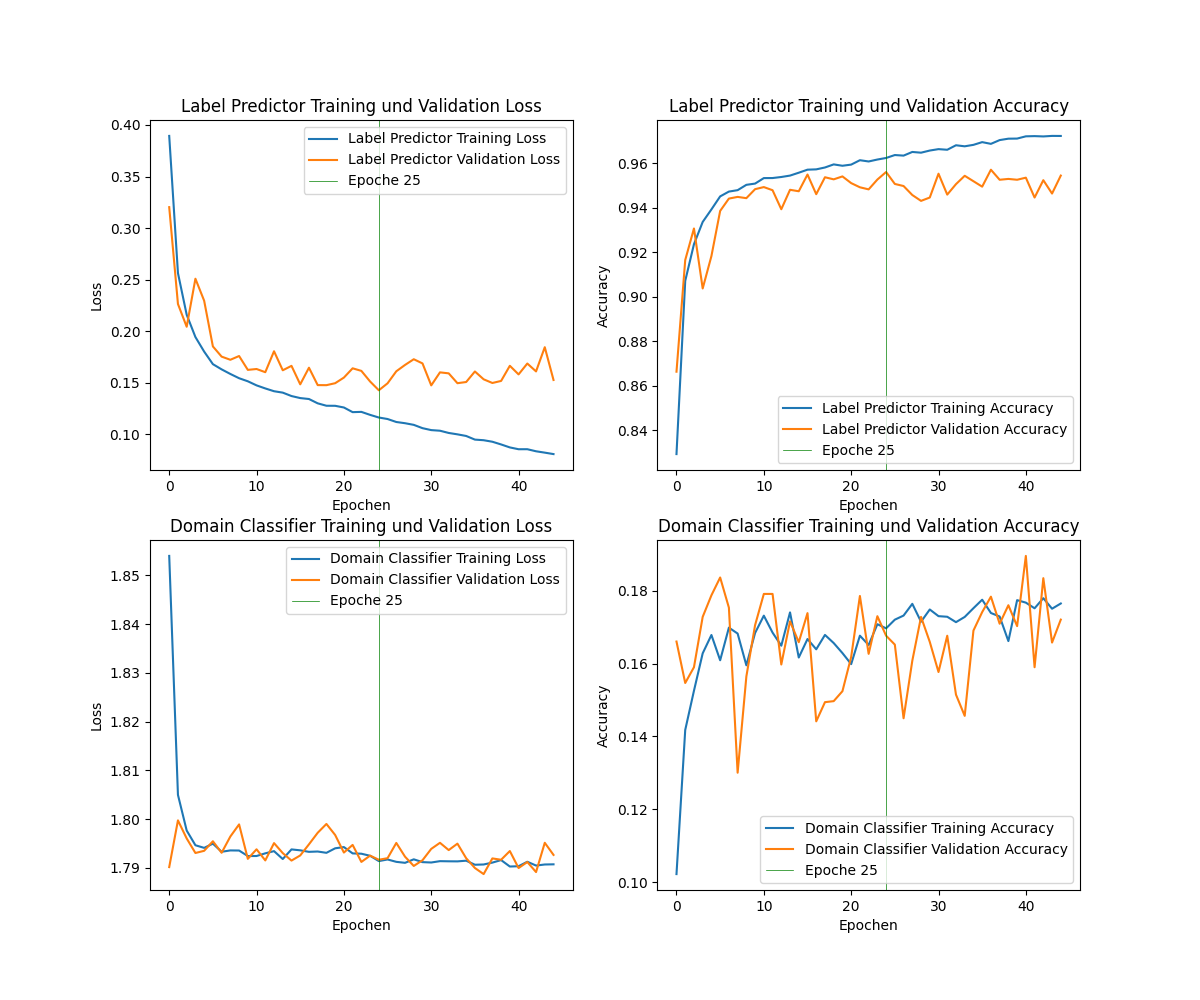
\includegraphics[width=1\textwidth]{./Bilder/DANN_training_fold1.png}
\caption[DANN Training Plots]{Trainings- und Validierungsverlauf des Label Predictors (oben) und des Domain Classifiers (unten) des \gls{DANN} Modells aus Fold 1 der Cross Validation. Epoche 25 ist die beste Epoche des Trainings.} 
\label{fig:DANN_training}
\end{figure} 

\subsection*{DANNdirect}

Für das \gls{DANN}direct wurde keine separate Grid Search durchgeführt, sondern es wurde diejenige Hyperparameterkombination für das Training genutzt, die bei der Grid Search des \gls{DANN} als am besten identifiziert wurde. Es erreicht mit 9 Inception Modulen, einer \texttt{learning rate} von 0,0001 und einer \texttt{batch size} von 32 einen F1-Score von 0,937 (bereinigt um $\sigma$ = 0,003), einen Recall von 0,932 (bereinigt um $\sigma$ = 0,009) und eine Specificity von 0,933 (bereinigt um $\sigma$ = 0,007). 

\subsection*{Vergleichsmodell InceptionTime}

Die vollständigen Ergebnisse der Grid Search des InceptionTime Modells sind im \hyperref[tab:GridSearch_InceptionTime]{Anhang A.1} zu finden. Die beste Hyperparameterkombination ist diejenige mit 9 Inception Modulen, einer \texttt{learning rate} von 0,0001 und einer \texttt{batch size} von 64. Die durchschnittlichen Werte der Modelle aus der Cross Validation sind ein F1-Score von 0,939 (bereinigt um $\sigma$ = 0,002), einen Recall von 0,935 (bereinigt um $\sigma$ = 0,006) und eine Specificity von 0,939 (bereinigt um $\sigma$ = 0,003).

\begin{table}[h!]
\centering
\caption[Ergebnisse der Evaluation auf der Quelldomäne xECGArch]{Evaluation der Modelle mit dem Testdatensatz der xECGArch-Datenbank. Globaler F1-Score der gewichteten und ungewichteten Ensembles, sowie Standardabweichung $\sigma$ und Durchschnittswert der Einzelmodelle. Der beste Wert ist hervorgehoben.}
\label{tab:Ergebnisse_indomain}
\begin{tabular}{lccccc}
\toprule
\textbf{Modell}       & \multicolumn{4}{c}{\textbf{xECGArch-Datenbank}} \\ 
\cmidrule(lr){2-5}
					  & \textbf{\makecell{F1 $\varnothing$ Modelle}} & \textbf{\makecell{$\sigma$}} & \textbf{\makecell{F1 Ensemble\\ gewichtet}} & \textbf{\makecell{F1 Ensemble\\ ungewichtet}} \\ \hline
\textbf{DANN} 			& 0,947           & 0,003            & \textbf{0,951}             & 0,950                   \\
\textbf{DANNdirect}     & 0,931           & 0,003            & 0,940             & 0,938 
\\
\textbf{InceptionTime}  & 0,930           & 0,002            & 0,938             & 0,938 
\\
\bottomrule
\end{tabular}
\end{table}

\section{Evaluierung auf Daten der Quelldomäne}\label{sec:quelldomäne}

\begin{table}[h!]
\centering
\caption[Ergebnisse der Evaluation auf der Quelldomäne xECGArch pro Ableitung]{Evaluation der Modelle mit dem Testdatensatz der xECGArch-Datenbank. Ergebnisse des gewichteten und ungewichteten Ensembles. Der jeweils beste F1-Score pro Ableitung ist hervorgehoben. }
\label{tab:Ergebnisse_indomain_leads}
\begin{tabular}{lccccccc}
\toprule
\textbf{Modell}     & \multicolumn{3}{c}{\textbf{Ensemble gewichtet}} & \multicolumn{3}{c}{\textbf{Ensemble ungewichtet}}\\
						& \textbf{F1} & \textbf{Recall} & \textbf{Specificity} & \textbf{F1} & \textbf{Recall} & \textbf{Specificity}\\  
\midrule
					   & \multicolumn{6}{c}{{Ableitung I}} \\ 
\cmidrule(lr){2-7}
\textbf{DANN} 			& \textbf{0,947}  & 0,933  & 0,960 & 0,945 & 0,935 & 0,954 \\
\textbf{DANNdirect}     & 0,931  & 0,935  & 0,923 & 0,928 & 0,931 & 0,921 \\
\textbf{InceptionTime}  & 0,929  & 0,929  & 0,925 & 0,930 & 0,931 & 0,925 \\
\midrule
					   & \multicolumn{6}{c}{{Ableitung II}} \\ 
\cmidrule(lr){2-7}
\textbf{DANN} 			& \textbf{0,954}  & 0,933  & 0,975 & \textbf{0,954} & 0,933 & 0,975 \\
\textbf{DANNdirect}     & 0,947  & 0,943  & 0,950 & 0,941 & 0,931 & 0,952 \\
\textbf{InceptionTime}  & 0,946  & 0,941  & 0,950 & 0,946 & 0,937 & 0,954 \\
\midrule
					   & \multicolumn{6}{c}{{ Ableitung III}} \\ 
\cmidrule(lr){2-7}
\textbf{DANN} 			& \textbf{0,946}  & 0,929  & 0,962 & 0,943 & 0,923 & 0,962 \\
\textbf{DANNdirect}     & 0,939  & 0,937  & 0,937 & 0,937 & 0,937 & 0,933 \\
\textbf{InceptionTime}  & 0,935  & 0,929  & 0,939 & 0,935 & 0,929 & 0,939 \\
\midrule
					   & \multicolumn{6}{c}{{ Ableitung aVR}} \\ 
\cmidrule(lr){2-7}
\textbf{DANN} 			& \textbf{0,962}  & 0,955  & 0,969 & 0,961 & 0,951 & 0,971 \\
\textbf{DANNdirect}     & 0,944  & 0,939  & 0,948 & 0,942 & 0,935 & 0,948 \\
\textbf{InceptionTime}  & 0,943  & 0,937  & 0,948 & 0,943 & 0,933 & 0,952 \\
\midrule
					   & \multicolumn{6}{c}{{ Ableitung aVL}} \\ 
\cmidrule(lr){2-7}
\textbf{DANN} 			& \textbf{0,944}  & 0,931  & 0,956 & 0,943 & 0,927 & 0,958 \\
\textbf{DANNdirect}     & 0,930  & 0,935  & 0,921 & 0,926 & 0,929 & 0,919 \\
\textbf{InceptionTime}  & 0,926  & 0,929  & 0,919 & 0,921 & 0,925 & 0,910 \\
\midrule
					   & \multicolumn{6}{c}{{ Ableitung aVF}} \\ 
\cmidrule(lr){2-7}
\textbf{DANN} 			& 0,956  & 0,939  & 0,973  & \textbf{0,957} & 0,941 & 0,973 \\
\textbf{DANNdirect}     & 0,950  & 0,945  & 0,952  & 0,953 & 0,949 & 0,956 \\
\textbf{InceptionTime}  & 0,950  & 0,949  & 0,948  & 0,950 & 0,947 & 0,952\\
\bottomrule
\end{tabular}
\end{table}


Die Modelle wurden auf dem Testdatensatz der xECGArch-Datenbank evaluiert. Auf diesen Datensatz hatten die Modelle während des Trainings keinen Zugriff. Zur Klassifikation wurden für alle \gls{EKG}s die Ableitungen I, II, III, aVR, aVL und aVF als eine gemischte Datenmenge eingegeben, analog zur Struktur des Trainingsdatensatzes. Der globale F1-Score wurde aus der Gesamtmenge der Vorhersagen gesammelt berechnet. Das dynamisch nach Klassifikationssicherheit der einzelnen Modelle gewichtete \gls{DANN} Ensemble erreicht mit 0,951 den besten globalen F1-Score. Die globalen F1-Scores der Ensembles, sowie den Durchschnitt der einzelnen Modelle der Ensembles und die Standardabweichung dieser lassen sich in \hyperref[tab:Ergebnisse_indomain]{Tab.~6.2} nachlesen. 

In den Abbildungen \hyperref[fig:DANN_label_roc]{6.2} und \hyperref[fig:DANN_label_roc]{6.3} sind als Beispiel die \gls{ROC}-Kurven des Label Predictors und des Domain Classifiers des \gls{DANN} Modells aus Fold 1 der Cross Validation dargestellt. Dabei fällt auf, dass die ROC-Kurve des Label Predictors des \gls{DANN} Modells eine große Fläche von 0,982 aufspannt, während die ROC-Kurven des Domain Classifiers des \gls{DANN} Modells nahe an der Winkelhalbierenden liegen und Flächen zwischen 0,477 bis 0,564 aufspannen.

Aufgeteilt nach Ableitung (siehe \hyperref[tab:Ergebnisse_indomain_leads]{Tab.~6.3}) wird der beste F1-Score mit 0,962 auf Ableitung aVR vom gewichteten \gls{DANN} Ensemble erreicht. Die durchschnittlichen F1-Scores der Ensembles über alle Ableitungen betragen für das \gls{DANN} 0,952 im gewichteten und 0,951 im ungewichteten Fall. Das gewichtete DANNdirect Ensemble erreicht einen durchschnittlichen F1-Score von 0,940 und das ungewichtete einen von 0,938. Das gewichtete und ungewichtete InceptionTime Ensemble erreichen einen durchschnittlichen F1-Score von 0,938. 



\begin{figure}[!ht]%
\centering
	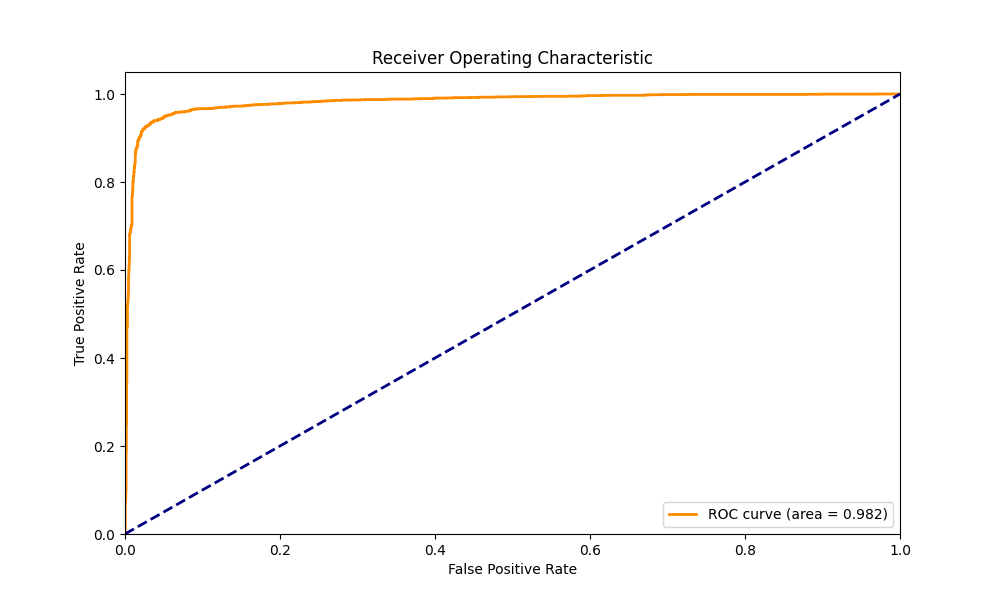
\includegraphics[width=0.8\textwidth]{./Bilder/DANN_roc_label_fold1.png}
\caption[Label Predictor ROC-Kurve]{Receiver-Operating-Characteristic-Kurve des Label Predictors des \gls{DANN} Modells aus Fold 1 der Cross Validation.} 
\label{fig:DANN_label_roc}
\end{figure}

\begin{figure}[!ht]%
\centering
	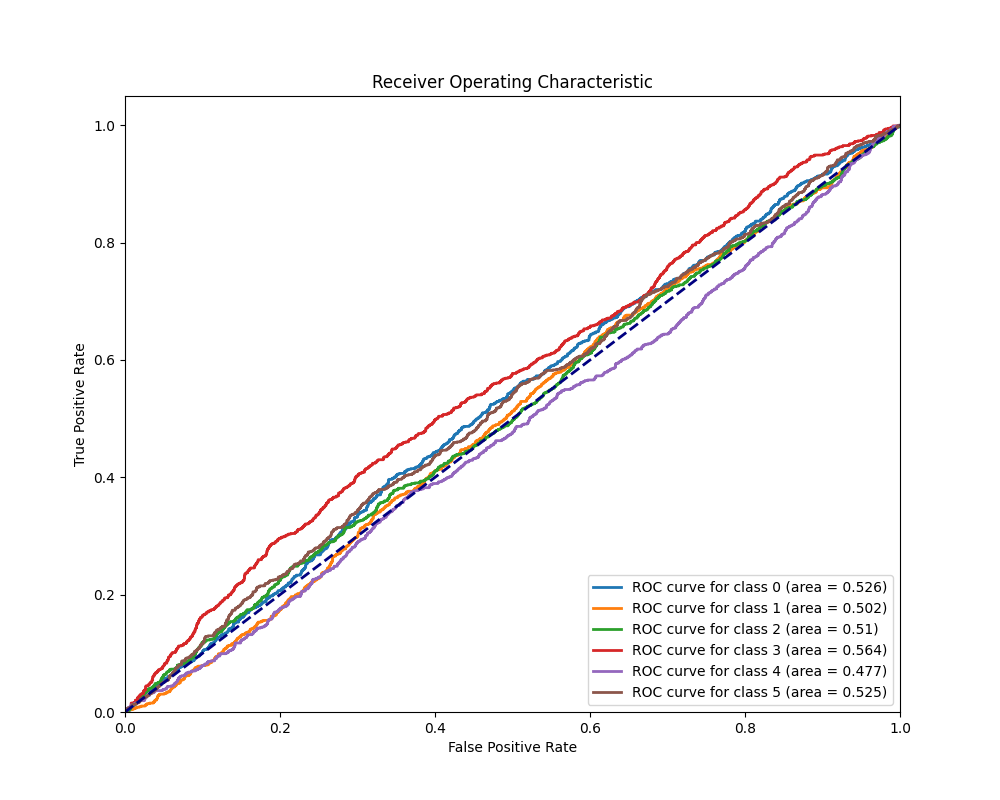
\includegraphics[width=0.8\textwidth]{./Bilder/DANN_roc_domain_fold1.png}
\caption[Domain Classifier ROC-Kurven]{Receiver-Operating-Characteristic-Kurve des Domain Classifiers des \gls{DANN} Modells aus Fold 1 der Cross Validation. } 
\label{fig:DANN_label_roc}
\end{figure}



\section{Evaluierung auf Daten der Zieldomänen}\label{sec:zieldomäne}

Um einzuschätzen, wie die Modelle mit einem Domain Shift umgehen, wurden die Modelle auf Daten von mobilen \gls{EKG}-Patches evaluiert, deren Signale eine andere Morphologie im Vergleich zu 12-Kanal-\gls{EKG}-Signalen aufweisen.

\subsubsection*{Icentia11k}

Bei der Icentia11k-Datenbank erreicht das ungewichtete \gls{DANN} Ensemble mit 0,666 den besten F1-Score (siehe \hyperref[tab:Ergebnisse_Icentia11k]{Tab.~6.4}) und den besten Recall mit 0,979. Die beste Specificity wird mit 0,952 sowohl vom ungewichteten als auch vom gewichteten \gls{DANN} Ensemble erreicht (siehe \hyperref[tab:sens_icentia]{Tab.~6.5}).

\begin{table}[h!]
\centering
\caption[Ergebnisse der Evaluation auf der Zieldomäne Icentia11k]{Evaluation der Modelle auf der Zieldomäne Icentia11k. F1-Score der gewichteten und ungewichteten Ensembles, sowie Standardabweichung $\sigma$ und Durchschnittswert der Einzelmodelle.}
\label{tab:Ergebnisse_Icentia11k}
\begin{tabular}{lccccc}
\toprule
\textbf{Modell}       & \multicolumn{4}{c}{\textbf{Icentia11k}} \\ 
\cmidrule(lr){2-5}
					  &\textbf{\makecell{F1 $\varnothing$ Modelle}} & \textbf{\makecell{$\sigma$}} & \textbf{\makecell{F1 Ensemble\\gewichtet}} & \textbf{\makecell{F1 Ensemble\\ungewichtet}} \\ \hline
\textbf{DANN} 			& 0,641           & 0,018            & 0,665             & \textbf{0,666}                   \\
\textbf{DANNdirect}     & 0,498           & 0,032            & 0,518             & 0,515 
\\
\textbf{InceptionTime}  & 0,520           & 0,013            & 0,543             & 0,541 
\\
\bottomrule
\end{tabular}
\end{table}


\begin{table}[h!]
\centering
\caption[Recall und Specificity Icentia11k]{Evaluation der Modelle auf der Zieldomäne Icentia11k. Recall und Specificity des gewichteten und ungewichteten Ensembles. }
\label{tab:sens_icentia}
\begin{tabular}{lccccc}
\toprule
\textbf{Modell}     & \multicolumn{2}{c}{\textbf{Ensemble gewichtet}} & \multicolumn{2}{c}{\textbf{Ensemble ungewichtet}}\\
						& \textbf{Recall} & \textbf{Specificity}  & \textbf{Recall} & \textbf{Specificity}\\  
\midrule
%					   & \multicolumn{4}{c}{{Ableitung 1}} \\ 
%\cmidrule(lr){2-5}
\textbf{DANN} 			& 0,973  & 0,952  & 0,979 & 0,952  \\
\textbf{DANNdirect}     & 0,947  & 0,915  & 0,943 & 0,915  \\
\textbf{InceptionTime}  & 0,936  & 0,925  & 0,936 & 0,924  \\

\bottomrule
\end{tabular}
\end{table}

\subsubsection*{TIMELY-Datensatz}

Die durchschnittliche Klassifikationsgüte der Ensembles auf dem TIMELY-Datensatz beträgt für das \gls{DANN} 0,973 (F1-Score) im gewichteten und 0,969 (F1-Score) im ungewichteten Fall. Das gewichtete DANNdirect Ensemble erreicht einen durchschnittlichen F1-Score von 0,948 und das ungewichtete einen von 0,947. Das gewichtete und das ungewichtete InceptionTime Ensemble erreichen jeweils einen durchschnittlichen F1-Score von 0,949.

Die Ergebnisse des TIMELY-Datensatzes wurden nach Ableitung aufgeschlüsselt. Auf allen drei Ableitungen erreicht jeweils das gewichtete \gls{DANN} Ensemble den besten F1-Score mit 0,952 auf Ableitung 1, 0,986 auf Ableitung 2 und 0,981 auf Ableitung 3 (siehe \hyperref[tab:Ergebnisse_timely]{Tab.~6.6}). Recall und Specificity der Modelle lässt sich aus \hyperref[tab:sens_timely]{Tab.~6.7} entnehmen.

\begin{table}[h!]
\centering
\caption[Ergebnisse der Evaluation auf der Zieldomäne TIMELY]{Evaluation der Modelle mit den drei Ableitungen des TIMELY-Datensatzes. F1-Score der gewichteten und ungewichteten Ensembles, sowie Standardabweichung $\sigma$ und Durchschnittswert der Einzelmodelle.}
\label{tab:Ergebnisse_timely}
\begin{tabular}{lccccc}
\toprule
\textbf{Modell}   & \textbf{\makecell{F1 $\varnothing$ Modelle}} & \textbf{\makecell{$\sigma$}} & \textbf{\makecell{F1 Ensemble\\gewichtet}} & \textbf{\makecell{F1 Ensemble\\ungewichtet}} \\     
			  
\midrule
 & \multicolumn{4}{c}{{TIMELY Ableitung 1}} \\   
\cmidrule(lr){2-5}
					  
\textbf{DANN} 			& 0,946           & 0,022            & \textbf{0,952}             & 0,942                   \\
\textbf{DANNdirect}     & 0,908           & 0,020            & 0,903             & 0,905 
\\
\textbf{InceptionTime}  & 0,908           & 0,026            & 0,904             & 0,905 
\\
\midrule

 		& \multicolumn{4}{c}{{TIMELY Ableitung 2}} \\ 
\cmidrule(lr){2-5}

\textbf{DANN} 			& 0,972           & 0,022            & \textbf{0,986}             & 0,985                   \\
\textbf{DANNdirect}     & 0,969           & 0,004            & 0,972             & 0,972 
\\
\textbf{InceptionTime}  & 0,971           & 0,004            & 0,976             & 0,975 
\\
\midrule
       & \multicolumn{4}{c}{{TIMELY Ableitung 3}} \\ 
\cmidrule(lr){2-5}

\textbf{DANN} 			& 0,972           & 0,006            & \textbf{0,981}             & 0,980                   \\
\textbf{DANNdirect}     & 0,959           & 0,005            & 0,969             & 0,965 
\\
\textbf{InceptionTime}  & 0,957           & 0,006            & 0,968             & 0,968 
\\
\bottomrule
\end{tabular}
\end{table}


\begin{table}[h!]
\centering
\caption[Recall und Specificity TIMELY]{Evaluation der Modelle auf der Zieldomäne TIMELY. Recall und Specificity des gewichteten und ungewichteten Ensembles. }
\label{tab:sens_timely}
\begin{tabular}{lccccc}
\toprule
\textbf{Modell}     & \multicolumn{2}{c}{\textbf{Ensemble gewichtet}} & \multicolumn{2}{c}{\textbf{Ensemble ungewichtet}}\\
						& \textbf{Recall} & \textbf{Specificity}  & \textbf{Recall} & \textbf{Specificity}\\  
\midrule
					   & \multicolumn{4}{c}{{TIMELY Ableitung 1}} \\ 
\cmidrule(lr){2-5}
\textbf{DANN} 			& 1,00  & 0,927  & 1,00 & 0,912  \\
\textbf{DANNdirect}     & 0,997  & 0,848  & 0,995 & 0,853  \\
\textbf{InceptionTime}  & 0,998  & 0,850  & 0,998 & 0,851  \\
\midrule
					   & \multicolumn{4}{c}{{TIMELY Ableitung 2}} \\ 
\cmidrule(lr){2-5}
\textbf{DANN} 			& 1,00  & 0,979  & 1,00 & 0,978  \\
\textbf{DANNdirect}     & 0,981  & 0,973  & 0,981 & 0,972  \\
\textbf{InceptionTime}  & 0,981  & 0,979  & 0,981 & 0,978  \\
\midrule
					   & \multicolumn{4}{c}{{TIMELY Ableitung 3}} \\ 
\cmidrule(lr){2-5}
\textbf{DANN} 			& 1,00  & 0,971  & 1,00 & 0,969  \\
\textbf{DANNdirect}     & 0,977  & 0,971  & 0,974 & 0,967  \\
\textbf{InceptionTime}  & 0,978  & 0,969  & 0,980 & 0,967  \\

\bottomrule
\end{tabular}
\end{table}

\subsubsection*{SHDB-AF}

Da 23 Patienten der \gls{SHDB-AF} während ihrer Aufnahme keine \gls{VHF}-Episode hatten, konnte für diese Patienten der Recall und somit der F1-Score nicht berechnet werden, sodass die Evaluierung nur für die übrigen 77 Patienten durchgeführt wurde. 
Bei der \gls{SHDB-AF} erreicht das \gls{DANN} Ensemble einen durchschnittlichen F1-Score von 0,815 im gewichteten und einen durchschnittlichen F1-Score von 0,810 im ungewichteten Fall. Das gewichtete DANNdirect Ensemble erreicht einen durchschnittlichen F1-Score von 0,755 und das ungewichtete einen durchschnittlichen F1-Score von 0,753. Für das gewichtete InceptionTime Ensemble beträgt der durchschnittliche F1-Score 0,757 und für das ungewichtete beträgt der durchschnittliche F1-Score 0,756.
Die Standardabweichung im F1-Score des gewichteten \gls{DANN} Ensembles zwischen den 77 Patienten mit \gls{VHF} beträgt 0,220.



In \hyperref[tab:Ergebnisse_shdb]{Tab.~6.8} und \hyperref[tab:sens_shdb]{Tab.~6.9} ist die Klassifikationsgüte der Modelle nach Ableitung aufgeschlüsselt. Auf den einzelnen Ableitungen erreicht das gewichtete \gls{DANN} den besten F1-Score mit 0,777 auf der CC5-Ableitung und 0,852 auf der NASA-Ableitung. 


\begin{table}[h!]
\centering
\caption[Ergebnisse der Evaluation auf der Zieldomäne SHDB-AF]{Evaluation der Modelle mit den zwei Ableitungen der SHDB-AF-Datenbank. F1-Score der gewichteten und ungewichteten Ensembles, sowie Standardabweichung $\sigma$ und Durchschnittswert der Einzelmodelle.}
\label{tab:Ergebnisse_shdb}
\begin{tabular}{lccccc}
\toprule
\textbf{Modell} & \textbf{\makecell{F1 $\varnothing$ Modelle}} & \textbf{\makecell{$\sigma$}} & \textbf{\makecell{F1 Ensemble\\gewichtet}} & \textbf{\makecell{F1 Ensemble\\ungewichtet}} \\   
\midrule
					& \multicolumn{4}{c}{{SHDB-AF CC5-Ableitung}} \\ 
\cmidrule(lr){2-5}
\textbf{DANN} 			& 0,763           & 0,014            & \textbf{0,777}             & 0,776                   \\
\textbf{DANNdirect}     & 0,694           & 0,028            & 0,717             & 0,715 
\\
\textbf{InceptionTime}  & 0,717           & 0,012            & 0,731             & 0,730 
\\
\midrule
       & \multicolumn{4}{c}{{SHDB-AF NASA-Ableitung}} \\ 
\cmidrule(lr){2-5}
	
\textbf{DANN} 			& 0,824           & 0,012            & \textbf{0,852}             & 0,844                   \\
\textbf{DANNdirect}     & 0,753           & 0,018            & 0,793             & 0,790 
\\
\textbf{InceptionTime}  & 0,753           & 0,012            & 0,783             & 0,781 
\\
\bottomrule
\end{tabular}
\end{table}



\begin{table}[h!]
\centering
\caption[Recall und Specificity SHDB-AF]{Evaluation der Modelle auf der Zieldomäne \gls{SHDB-AF}. Recall und Specificity des gewichteten und ungewichteten Ensembles. }
\label{tab:sens_shdb}
\begin{tabular}{lccccc}
\toprule
\textbf{Modell}     & \multicolumn{2}{c}{\textbf{Ensemble gewichtet}} & \multicolumn{2}{c}{\textbf{Ensemble ungewichtet}}\\
						& \textbf{Recall} & \textbf{Specificity}  & \textbf{Recall} & \textbf{Specificity}\\  
\midrule
					   & \multicolumn{4}{c}{{CC5-Ableitung}} \\ 
\cmidrule(lr){2-5}
\textbf{DANN} 			& 0,949  & 0,947  & 0,949 & 0,947  \\
\textbf{DANNdirect}     & 0,948  & 0,904  & 0,946 & 0,903  \\
\textbf{InceptionTime}  & 0,951  & 0,912  & 0,948 & 0,914  \\
\midrule
					   & \multicolumn{4}{c}{{NASA-Ableitung}} \\ 
\cmidrule(lr){2-5}
\textbf{DANN} 			& 0,933  & 0,944  & 0,932 & 0,944  \\
\textbf{DANNdirect}     & 0,925  & 0,916  & 0,922 & 0,915  \\
\textbf{InceptionTime}  & 0,920  & 0,920  & 0,918 & 0,920  \\

\bottomrule
\end{tabular}
\end{table}

\section{Untersuchung des Einflusses der Normalisierung der Daten }\label{sec:nichtnormalisiert}

Im Rahmen dieser Arbeit wurden ebenfalls Modelle trainiert, ohne zuvor die Trainingsdaten zu z-normalisieren. Die beste Hyperparameterkombination dieser Modelle wurde ebenfalls per Grid Search ermittelt. Für das \gls{DANN} wurde als optimale Hyperparameterkombination 9 Inception Module, eine \texttt{learning rate} von 0,0001 und eine \texttt{batch size} von 64 ermittelt. Der durchschnittliche F1-Score abzüglich der Standardabweichung aus den Modellen der Cross Validation beträgt 0,956. Die Standardabweichung beträgt 0,002. Das DANNdirect wurde anschließend mit derselben Hyperparameterkombination trainiert.

Für InceptionTime wurde als optimale Hyperparameterkombination eine Anzahl von 9 Inception Modulen, eine \texttt{learning rate} von 0,001 und eine \texttt{batch size} von 128 ermittelt. Der durchschnittliche F1-Score abzüglich der Standardabweichung der InceptionTime Modelle aus der Cross Validation beträgt 0,941. Die Standardabweichung beträgt 0,003. 

Die Modelle wurden auf dem nicht normalisierten xECGArch-Testdatensatz evaluiert. Die höchste Klassifikationsgüte erreichen das gewichtete und ungewichtete \gls{DANN} Ensemble mit einem globalen F1-Score von 0,953 (siehe \hyperref[tab:Ergebnisse_indomain_notnorm]{Tab.~6.10}). Anschließend wurden die Modelle auf dem nicht-normalisierten TIMELY-Datensatz angewendet, um zu evaluieren, wie sie sich bei einem Domain Shift verhalten. In \hyperref[tab:Ergebnisse_timely_notnorm]{Tab.~6.11} ist die Klassifikationsgüte der Modelle für jede Ableitung des Datensatzes eingetragen. Die durchschnittlich höchste Klassifikationsgüte erreicht das \gls{DANN} Ensemble mit einem F1-Score von 0,946. 

\begin{table}[h!]
\centering
\caption[Ergebnisse der Evaluation auf der Quelldomäne mit nicht-normalisierten Daten]{Evaluation der Modelle mit dem nicht-normalisierten Testdatensatz der xECGArch-Datenbank. Globaler F1-Score der gewichteten und ungewichteten Ensembles, sowie Standardabweichung $\sigma$ und Durchschnittswert der Einzelmodelle. Der beste Wert ist hervorgehoben.}
\label{tab:Ergebnisse_indomain_notnorm}
\begin{tabular}{lccccc}
\toprule
\textbf{Modell}       & \multicolumn{4}{c}{\textbf{xECGArch-Datenbank}} \\ 
\cmidrule(lr){2-5}
					  & \textbf{\makecell{F1 $\varnothing$ Modelle}} & \textbf{\makecell{$\sigma$}} & \textbf{\makecell{F1 Ensemble\\ gewichtet}} & \textbf{\makecell{F1 Ensemble\\ ungewichtet}} \\ \hline
\textbf{DANN} 			& 0,948  & 0,003  & \textbf{0,953}  & \textbf{0,953}   \\
\textbf{DANNdirect}     & 0,932  & 0,003  & 0,937  & 0,938 \\
\textbf{InceptionTime}  & 0,934  & 0,003  & 0,942  & 0,942 \\
\bottomrule
\end{tabular}
\end{table}

\begin{table}[h!]
\centering
\caption[Ergebnisse der Evaluation auf nicht-normalisierten TIMELY-Daten]{Evaluation der Modelle mit den drei nicht-normalisierten Ableitungen des TIMELY-Datensatzes. F1-Score der gewichteten und ungewichteten Ensembles, sowie Standardabweichung $\sigma$ und Durchschnittswert der Einzelmodelle.}
\label{tab:Ergebnisse_timely_notnorm}
\begin{tabular}{lccccc}
\toprule
\textbf{Modell}   & \textbf{\makecell{F1 $\varnothing$ Modelle}} & \textbf{\makecell{$\sigma$}} & \textbf{\makecell{F1 Ensemble\\gewichtet}} & \textbf{\makecell{F1 Ensemble\\ungewichtet}} \\     
			  
\midrule
 & \multicolumn{4}{c}{{TIMELY Ableitung 1}} \\   
\cmidrule(lr){2-5}
					  
\textbf{DANN} 			& 0,935 & 0,014 & \textbf{0,949} & 0,947  \\
\textbf{DANNdirect}     & 0,892 & 0,022 & 0,891 & 0,892 \\
\textbf{InceptionTime}  & 0,902 & 0,025 & 0,916 & 0,915 \\
\midrule

 		& \multicolumn{4}{c}{{TIMELY Ableitung 2}} \\ 
\cmidrule(lr){2-5}

\textbf{DANN} 			& 0,938  & 0,036    & 0,921  & 0,917  \\
\textbf{DANNdirect}     & 0,931  & 0,039   & 0,940   & 0,961 \\
\textbf{InceptionTime}  & 0,952  & 0,007    & \textbf{0,967}  & 0,966 \\
\midrule
       & \multicolumn{4}{c}{{TIMELY Ableitung 3}} \\ 
\cmidrule(lr){2-5}

\textbf{DANN} 			& 0,936  & 0,022   & \textbf{0,968}   & 0,962 \\
\textbf{DANNdirect}     & 0,920  & 0,023   & 0,949   & 0,945 \\
\textbf{InceptionTime}  & 0,903  & 0,022   & 0,936   & 0,931 \\
\bottomrule
\end{tabular}
\end{table}
 \newpage
\chapter{Diskussion}\label{chap:diskussion}

Ziel dieser Arbeit war die Entwicklung eines Modells zur \gls{VHF}-Detektion im \gls{EKG}, das robust gegen veränderte Signalmorphologie ist. Dazu wurden 3 Modelle (\gls{DANN}, DANNdirect und InceptionTime) trainiert und auf Daten der Quell- und der Zieldomäne getestet. Die entsprechenden Ergebnisse werden in diesem Kapitel eingeordnet und diskutiert. In \hyperref[sec:einordnung]{Abschnitt 7.1} wird zunächst die Klassifikationsgüte der Modelle auf der Quelldomäne eingeordnet. In \hyperref[sec:diskhyper]{Abschnitt 7.2} werden die Ergebnisse der Hyperparameteroptimierung und in \hyperref[sec:disktest]{Abschnitt 7.3} die Ergebnisse auf den Testdatensätzen diskutiert. Zuletzt wird in \hyperref[sec:disknorm]{Abschnitt 7.4} der Einfluss von Normalisierung diskutiert.

\section{Allgemeine Einordnung der Klassifikationsgüte der Modelle}\label{sec:einordnung}

Der Trainingsverlauf in \hyperref[fig:DANN_training]{Abb.~6.1} zeigt, dass das \gls{DANN} wie erwartet trainiert. Der Loss des Label Predictors sinkt im Verlauf des Trainings bis Epoche 25, nach welcher per Early Stopping das Training beendet wurde, während der Loss des Domain Classifiers konstant hoch blieb. Die \gls{ROC}-Kurven von Label Predictor (siehe \hyperref[fig:DANN_label_roc]{Abb.~6.2}) und Domain Classifier (siehe \hyperref[fig:DANN_domain_roc]{Abb.~6.3}) zeigen ebenfalls, dass das Modell in der Lage ist, die Hauptklassifikationsaufgabe auszuführen, während der Domain Classifier nicht in der Lage ist, die einzelnen Ableitungen zu differenzieren. Die Fläche, die durch die \gls{ROC}-Kurve des Label Predictors aufgespannt wird, ist mit 0,982 sehr groß, was laut \cite{mandrekar_receiver_2010} als sehr gut eingeordnet werden kann. Die Teilhypothesen a) und b) konnten somit bewiesen werden.

Werden die einzelnen Modelle zu einem ungewichteten Ensemble kombiniert, erhöht sich die Gesamtgüte (siehe \hyperref[tab:Ergebnisse_indomain]{Tab.~6.2}). Gewichtet man das Ensemble, erhöht sich die Klassifikationsgüte noch einmal. Teilhypothese d) wurde somit bestätigt.

Teilhypothese e) besagt, dass das \gls{DANN} auf dem xECGArch-Testdatensatz eine geringere Klassifikationsgüte erzielen sollte als das Vergleichsmodell, da es aufgrund des Domain Adversarial Learnings weniger stark overfittet. Dies konnte nicht nachgewiesen werden, da sowohl die einzelnen Modelle als auch beide \gls{DANN} Ensembles auf dem Testdatensatz der 12-Kanal-\gls{EKG}s eine höhere  Klassifikationsgüte erzielen als das Vergleichsmodell. Dies lässt sich durch die Tatsache erklären, dass die 12-Kanal-\gls{EKG}s nicht insgesamt, sondern jeweils nur ein einzelner Kanal als Eingabe der Modelle genutzt wurde. Zwischen den einzelnen Kanälen existieren morphologische Unterschiede, sodass Domain Adversarial Learning auch hier dazu beiträgt, universelle Merkmale zu erlernen.

Das von Goettling et al. \cite{goettling_xecgarch_2024} entwickelte Modell xECGArch, dessen Trainings- und Testdatensatz in dieser Arbeit verwendet wurde, nutzt Ableitung II für Training und Evaluation. Es erreicht bei der Detektion von \gls{VHF} einen F1-Score von 0,954, sowie einen Recall von 0,949 und eine Specificity von 0,958. Das gewichtete \gls{DANN} Ensemble, welches mit den 6 Extremitätenableitungen des xECGArch-Datensatzes trainiert wurde, erreicht auf Ableitung II ebenfalls einen F1-Score von 0,954, sowie einen etwas geringeren Recall von 0,933 und eine etwas höhere Specificity von 0,975. Aus dem Vergleich der F1-Scores lässt sich schließen, dass das gewichtete \gls{DANN} Ensemble eine vergleichbare Klassifikationsgüte wie xECGArch aufweist. Der leicht niedrigere Recall, sowie die leicht höhere Specificity deuten darauf hin, dass das gewichtete \gls{DANN} Ensemble minimal weniger wahre \gls{VHF}-Episoden detektiert und dabei weniger falsch positive Ergebnisse erreicht. In der klinischen Praxis ist wünschenswert, einen höheren Recall zu erreichen und alle tatsächlichen \gls{VHF}-Fälle zu erkennen und dafür falsch positive Detektionen in kauf zu nehmen. Recall und Specificity von über 0,900 können nach \cite{plante_selection_1994} dennoch als sehr gut eingeordnet werden.   

Ribeiro et al. \cite{ribeiro_automatic_2020} haben im Rahmen ihrer Arbeit die Klassifikationsgüte von Menschen zusätzlich zur Klassifikationsgüte ihres \gls{DNN}s erhoben. Assistenzärzte für Kardiologie im vierten Jahr erreichten einen F1-Score von 0,769 in der Erkennung von \gls{VHF} in 12-Kanal-\gls{EKG}s. Das gewichtete \gls{DANN} Ensemble erreicht auf 12-Kanal-\gls{EKG}s einen F-Score von 0,951. Es erzielt also eine höhere Klassifikationsgüte, als die von Ribeiro et al. getesteten Ärzte, wobei beachtet werden muss, dass es sich um verschiedene 12-Kanal-\gls{EKG}-Datenbanken handelt. 

Insgesamt muss angemerkt werden, dass es sich bei dem in dieser Arbeit genutzten Ansatz nicht um einen erklärbaren Ansatz handelt. Dies bedeutet, dass zwar Vermutungen angestellt werden können, welche Merkmale vom Modell zur Vorhersage genutzt werden (bspw. Rhythmus-Merkmale im Fall von Filtern mit großem Wahrnehmungsbereich und morphologische Merkmale im Fall von Filtern mit kleinerem Wahrnehmungsbereich), jedoch keine Methode umgesetzt wurde, um dies zu überprüfen.

Weiterhin muss angemerkt werden, dass bei der Vorverarbeitung der Datensätze nicht bedacht wurde, dass die Netzfrequenz in Nordamerika bei 60~Hz liegt und somit alle Datensätze mit einem Powerline Filter mit der Frequenz 50~Hz gefiltert wurden. Jedoch hat dies auf die Klassifikationsgüte vermutlich nur einen geringen Einfluss, da sowohl Daten aus Ländern mit einer Netzfrequenz von 60~Hz, als auch Daten aus Ländern mit einer Netzfrequenz von 50~Hz im Trainingsdatensatz vertreten sind.   

\section{Ergebnisse der Hyperparameteroptimierung}\label{sec:diskhyper}

Einige Hyperparameterkombinationen aus der \gls{DANN} Grid Search, insbesondere jene mit einer \texttt{learning rate} von 0,01 besitzen eine besonders geringe  Klassifikationsgüte (siehe \hyperref[tab:GridSearch_DANN]{Tab.~6.1}). Dabei fällt auf, dass diese Modelle alle denselben F1-Score von -0,134 (Mittelwert - $\sigma$) besitzen und sich auch in den restlichen Metriken nicht unterscheiden. Die negativen Werte in der Tabelle kommen zustande, wenn die Standardabweichung zwischen den 5 Modellen der Cross Validation größer ist als der Durchschnittswert. Es kann vorkommen, dass bspw. durch Probleme mit einzelnen Knoten Jobs auf einem \gls{HPC} nicht korrekt ausgeführt werden. Um sicherzugehen, dass die schlechten Werte nicht durch einen Fehler während der Berechnung auf dem \gls{HPC} zustande kamen, wurde ein zusätzliches Modell mit einer dieser Hyperparameterkombinationen auf einem anderen Knoten trainiert, welches dasselbe Ergebnis lieferte. Die schlechten Werte entstehen durch Modelle, die am Ende des Trainingsvorgangs nur in der Lage sind, einen einzigen Wert vorherzusagen (entweder nur 0 oder nur 1). Vermutlich durch die geringe \texttt{learning rate} ausgelöst, hängen diese Modelle in einem lokalen Minimum fest. Sind weniger Inception Module im Modell vorhanden, ist auch eine \texttt{learning rate} von 0,001 zu gering, um die Modelle erfolgreich zu trainieren. Eine Anzahl von 9 Inception Modulen gleicht 0,001 als \texttt{learning rate} aus.


Das \gls{DANN}direct Ensemble hat keine wesentlich höhere Klassifikationsgüte als das InceptionTime Ensemble. Dabei sollte berücksichtigt werden, dass für das Training der \gls{DANN}direct Modelle keine zusätzliche Grid Search durchgeführt wurde, sondern die Ergebnisse der Hyperparameteroptimierung des \gls{DANN}s genutzt wurden. Dadurch könnten die Hyperparameter des \gls{DANN}direct Ensembles suboptimal sein, was die Klassifikationsgüte der Modelle beeinträchtigt haben könnte. Das Entfernen der \gls{FC}-Layer des Label Predictors könnte ebenfalls die Klassifikationsgüte beeinträchtigt haben, da die \gls{FC}-Layer dazu beitragen, die Features aus dem Feature Extractor zu kombinieren und für die Klassifikation zu optimieren. 


\section{Diskussion der Ergebnisse auf unterschiedlichen Testdatensätzen}\label{sec:disktest}

\subsection*{Icentia11k}

Auf dem Icentia11-Datensatz liegt der F1-Score des gewichteten \gls{DANN} Ensembles bei 0,665 und ist somit im Vergleich zu den F1-Scores auf dem xECGArch Datensatz (0,944-0,956) deutlich schlechter. Recall und Specificity liegen bei 0,973 und 0,952 und sind damit relativ hoch. Der hohe Recall zeigt, dass das Ensemble fast alle \gls{VHF}-Fälle erkennt, eine hohe Specificity bedeutet, dass das Ensemble auch die meisten gesunden Patienten korrekt klassifiziert. Der dennoch niedrige F1-Score lässt sich durch die große Anzahl an falsch-positiven Klassifikationen erklären. Von insgesamt 513 \gls{VHF}-Fällen erkennt das Ensemble 499 korrekt, jedoch werden zusätzlich 489 negative \gls{EKG}s fälschlicherweise als \gls{VHF} klassifiziert. Der Icentia11k-Datensatz ist sehr unausgeglichen und enthält mit 10~689 viele negative und mit 513 nur sehr wenige positive \gls{VHF}-Fälle. Bei unausgeglichenen Datensätzen mit vielen negativen Fällen ist die Specificity keine zuverlässige Metrik, da es viele negative Fälle gibt, die korrekt negativ erkannt werden können.   

Ein Grund für die falsch positiven Klassifikationen kann die Auflösung der Icentia11k-\gls{EKG}-Signale sein. Sie ist teilweise sehr gering, sodass davon ausgegangen werden kann, dass die Modelle nur die R-Zacken und somit nur Rhythmusmerkmale extrahieren und zur Klassifikation nutzen konnten und keine morphologischen Merkmale, was den Abfall in der Klassifikationsleistung erklären kann. Ein Beispiel für eine Aufnahme mit geringer Auflösung ist in  \hyperref[fig:icentia_plot]{Abb.~7.1} zu sehen. Zusätzlich gibt es eine große Anzahl an verrauschten Signalen wie in \hyperref[fig:icentia_plot]{Abb.~7.2} dargestellt, die die Klassifikationsgüte beeinflusst haben könnte. 

\begin{figure}[!ht]%
\centering
	\includegraphics[width=1\textwidth]{./Bilder/icentia_geringe_auflösung.png}
\caption[Plot einer Icentia11k-Aufnahme mit geringer Auflösung]{Eine Aufnahme entnommen von Patient 09322 aus der Icentia11k-Datenbank. Sie wurde als Vorhofflimmern annotiert und vom \gls{DANN} Ensemble falsch klassifiziert. Zu sehen ist, dass die Aufnahme sehr gering aufgelöst ist.} 
\label{fig:icentia_plot}
\end{figure} 

\begin{figure}[!ht]%
\centering
	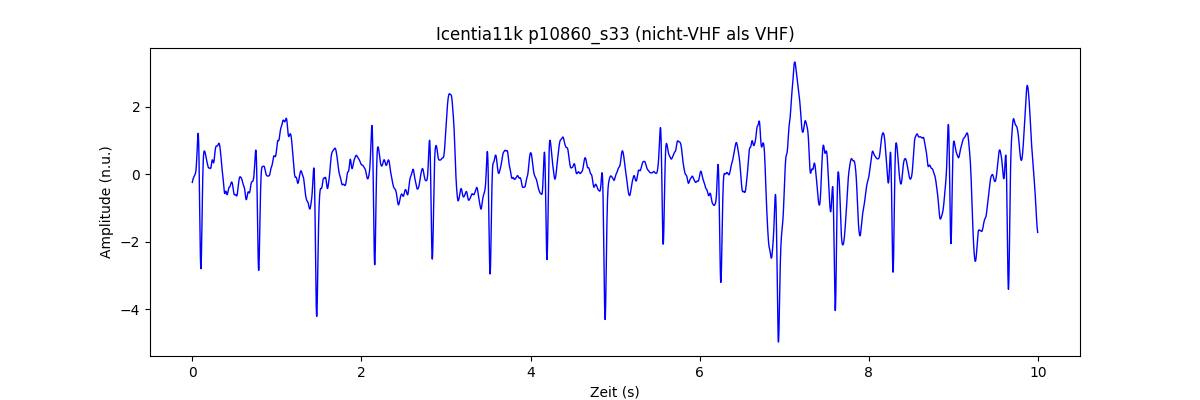
\includegraphics[width=1\textwidth]{./Bilder/icentia_verrauscht.png}
\caption[Plot einer verrauschten Icentia11k-Aufnahme]{Eine Aufnahme entnommen von Patient 10860 aus der Icentia11k-Datenbank. Sie wurde als normaler Sinusrhythmus annotiert und vom \gls{DANN} Ensemble falsch klassifiziert. Zu sehen ist, dass die Aufnahme verrauscht ist.} 
\label{fig:icentia_plot2}
\end{figure} 

\subsection*{TIMELY-Datensatz}

Das gewichtete \gls{DANN} Ensemble erzielt auf allen drei Ableitungen des TIMELY-Datensatzes einen F1-Score von 0,952-0,986, der laut \cite{plante_selection_1994} als sehr gut eingeordnet werden kann. Damit erzielt das Ensemble eine höhere Klassifikationsgüte auf einer signalmorphologisch veränderten Zieldomäne als das Modell von Ramesh et al. \cite{ramesh_atrial_2021}. Dieses Modell erreicht auf der Quelldomäne \gls{EKG} einen F1-Score von 0,93 und auf der Zieldomäne \gls{PPG}, die ein morphologisch verändertes Signal darstellt, mit Transfer Learning einen F1-Score von 0,89.

Des Weiteren erreicht das gewichtete \gls{DANN} Ensemble den bestmöglichen Recall von 1,00. Dies bedeutet, dass alle \gls{VHF}-Fälle korrekt als \gls{VHF} klassifiziert wurden. Zusammen mit einer hohen durchschnittlichen Specificity von 0,959 und einem hohen F1-Score lässt sich die Aussage treffen, dass es keine übermäßig hohen falsch positiven Klassifikationen gibt. 
Anzumerken ist hier, dass, obwohl die TIMELY-Ableitungen bei richtiger Positionierung der Elektroden modifizierte Einthoven-Ableitungen sind, dies in der Praxis nicht zutrifft. Die Morphologie der einzelnen Ableitungen variiert stark mit der Platzierung und Rotation des \gls{EKG}-Patches. Da die Patienten selbst den Patch angebracht haben, kam es vor, dass der Patch nicht über dem Herzen saß oder unter Umständen rotiert angebracht wurde, wodurch Ableitungen morphologisch verändert oder gar vertauscht sein können. Daraus lässt sich schließen, dass das Aufschlüsseln der Klassifikationsgüte nach Ableitung nicht sinnvoll ist und die Beurteilung der Klassifikationsgüte des Modells auf dem Durchschnittswert stattfinden sollte. Da auch der durchschnittliche F1-Score mit 0,973 sehr gut ist, kann Teilhypothese c) als bestätigt angesehen werden. Die Haupthypothese wurde bewiesen, da die Klassifikationsgüte des gewichteten \gls{DANN} Ensembles höher ist als die Klassifikationsgüte des gewichteten InceptionTime Ensembles (F1-Score von 0,949).

\subsection*{SHDB-AF}
Es fällt auf, dass die Klassifikationsgüte der Modelle auf der \gls{SHDB-AF} Datenbank auf der CC5-Ableitung wesentlich schlechter ist, als auf der NASA-Ableitung (F1-Scores von 0,717-0,777 vs. F1-Scores von 0,783-0,852). Die Ursache hierfür liegt darin, dass es sich bei der CC5-Ableitung um eine Brustwandableitung handelt. Für das Training der Modelle wurden nur die Ableitungen I, II, III, aVR, aVL und aVF genutzt, jedoch nicht die 6 Brustwandableitungen. Somit ist der Domain Shift zwischen den Trainingsdaten und der CC5-Ableitung der \gls{SHDB-AF} Datenbank größer als der zwischen den Trainingsdaten und der NASA-Ableitung der \gls{SHDB-AF} Datenbank und ein Abfall der Klassifikationsleistung der Modelle zu erwarten.

\begin{figure}[!ht]%
\centering
	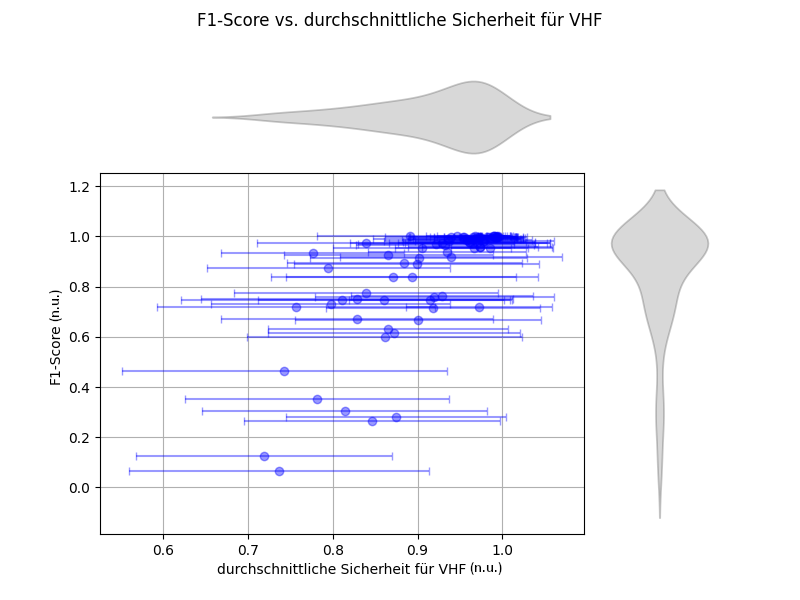
\includegraphics[width=1\textwidth]{./Bilder/shdb_plot_vhf.png}
\caption[SHDB-AF F1-Score vs. durchschnittliche Sicherheit für VHF]{F1-Score für die \gls{VHF}-Klasse gegen die durchschnittliche Sicherheit des gewichteten \gls{DANN} Ensembles pro Patient aufgetragen. Zusätzlich ist die Standardabweichung der Sicherheit pro Patient in Form von T-Balken eingetragen. Anhand des Violinenplots lässt sich die Verteilung der F1-Scores bzw. der durchschnittlichen Sicherheit für die Klassifikation über die Aufnahmen ablesen. } 
\label{fig:shdb_scatter_vhf}
\end{figure} 

Desweiteren ist die Standardabweichung der F1-Scores für \gls{VHF} innerhalb der 77 Patienten, die während der Aufzeichnung eine \gls{VHF}-Episode hatten, relativ hoch. Als Beispiel werden nun die Ergebnisse des gewichteten \gls{DANN} Ensembles auf der NASA-Ableitung betrachtet. Hier beträgt die Standardabweichung für die \gls{VHF}-Klasse 0,220. Die Standardabweichung der F1-Scores für die nicht-\gls{VHF}-Klasse innerhalb derselben 77 Patienten ist mit 0,191 vergleichbar hoch. 


In \hyperref[fig:shdb_scatter_vhf]{Abb.~7.3} ist der F1-Score für die \gls{VHF}-Klasse gegen die durchschnittliche Sicherheit des Ensembles pro Patient aufgetragen. Zusätzlich ist die Standardabweichung der Sicherheit pro Patient in Form von T-Balken eingetragen. Zu sehen ist, dass der Großteil der Teil Aufnahmen mit einem guten F1-Score und einer hohen durchschnittlichen Sicherheit klassifiziert werden konnte. Jedoch gibt es einige Patienten, deren Aufnahmen einen sehr geringen F1-Score und auch eine geringere Sicherheit in der Klassifikation aufweisen. Auf einige dieser Aufnahmen wird nun eingegangen.

\begin{figure}[!ht]%
\centering
	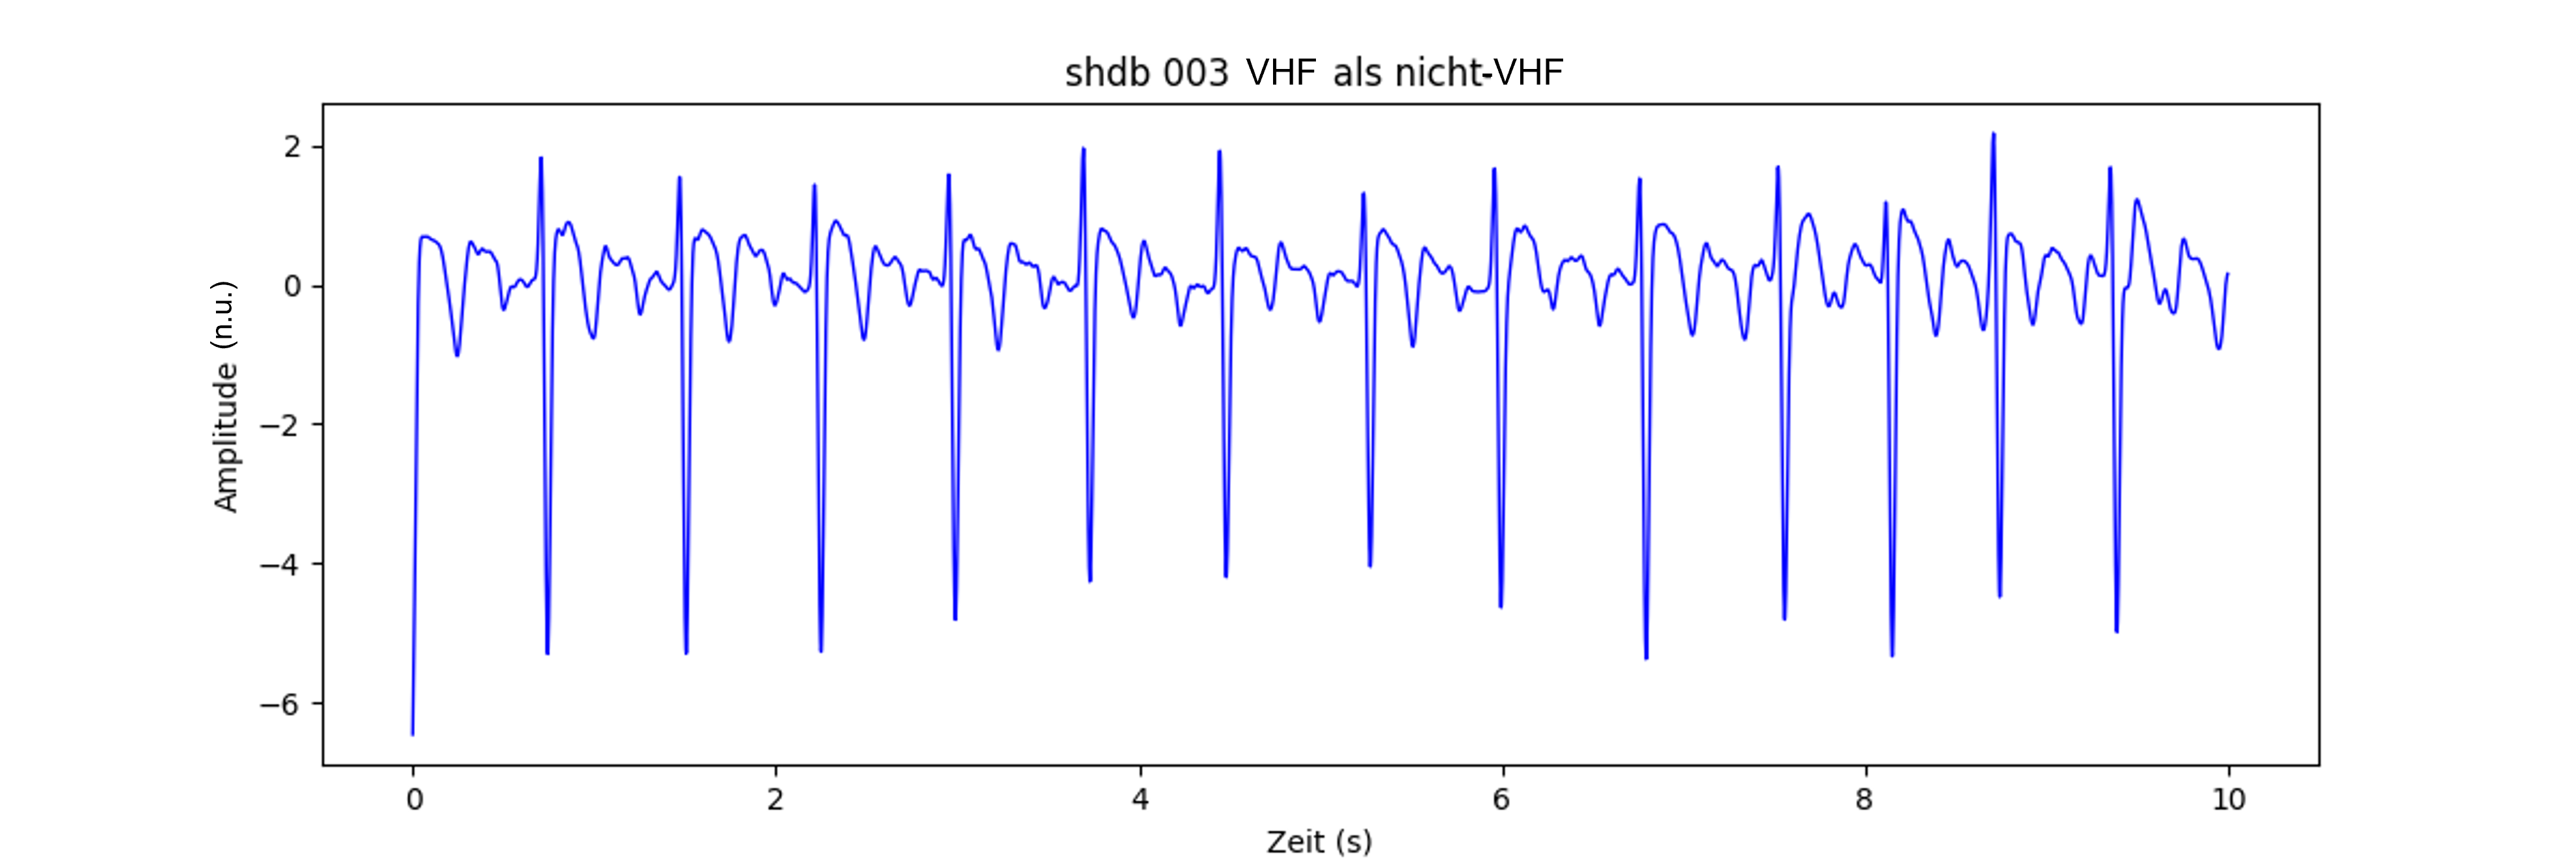
\includegraphics[width=1\textwidth]{./Bilder/003_vhf.png}
\caption[SHDB-AF Aufnahme von Patient 003 mit AFIB Annotation]{Eine Aufnahme von Patient 003 aus der SHDB-AF Datenbank, welche mit \gls{VHF} Annotiert und als nicht-\gls{VHF} vom gewichteten \gls{DANN} Ensemble klassifiziert wurde. Zu sehen ist eine regelmäßige Vorhoferregung.} 
\label{fig:shdb_003_vhf}
\end{figure} 

\begin{figure}[!ht]%
\centering
	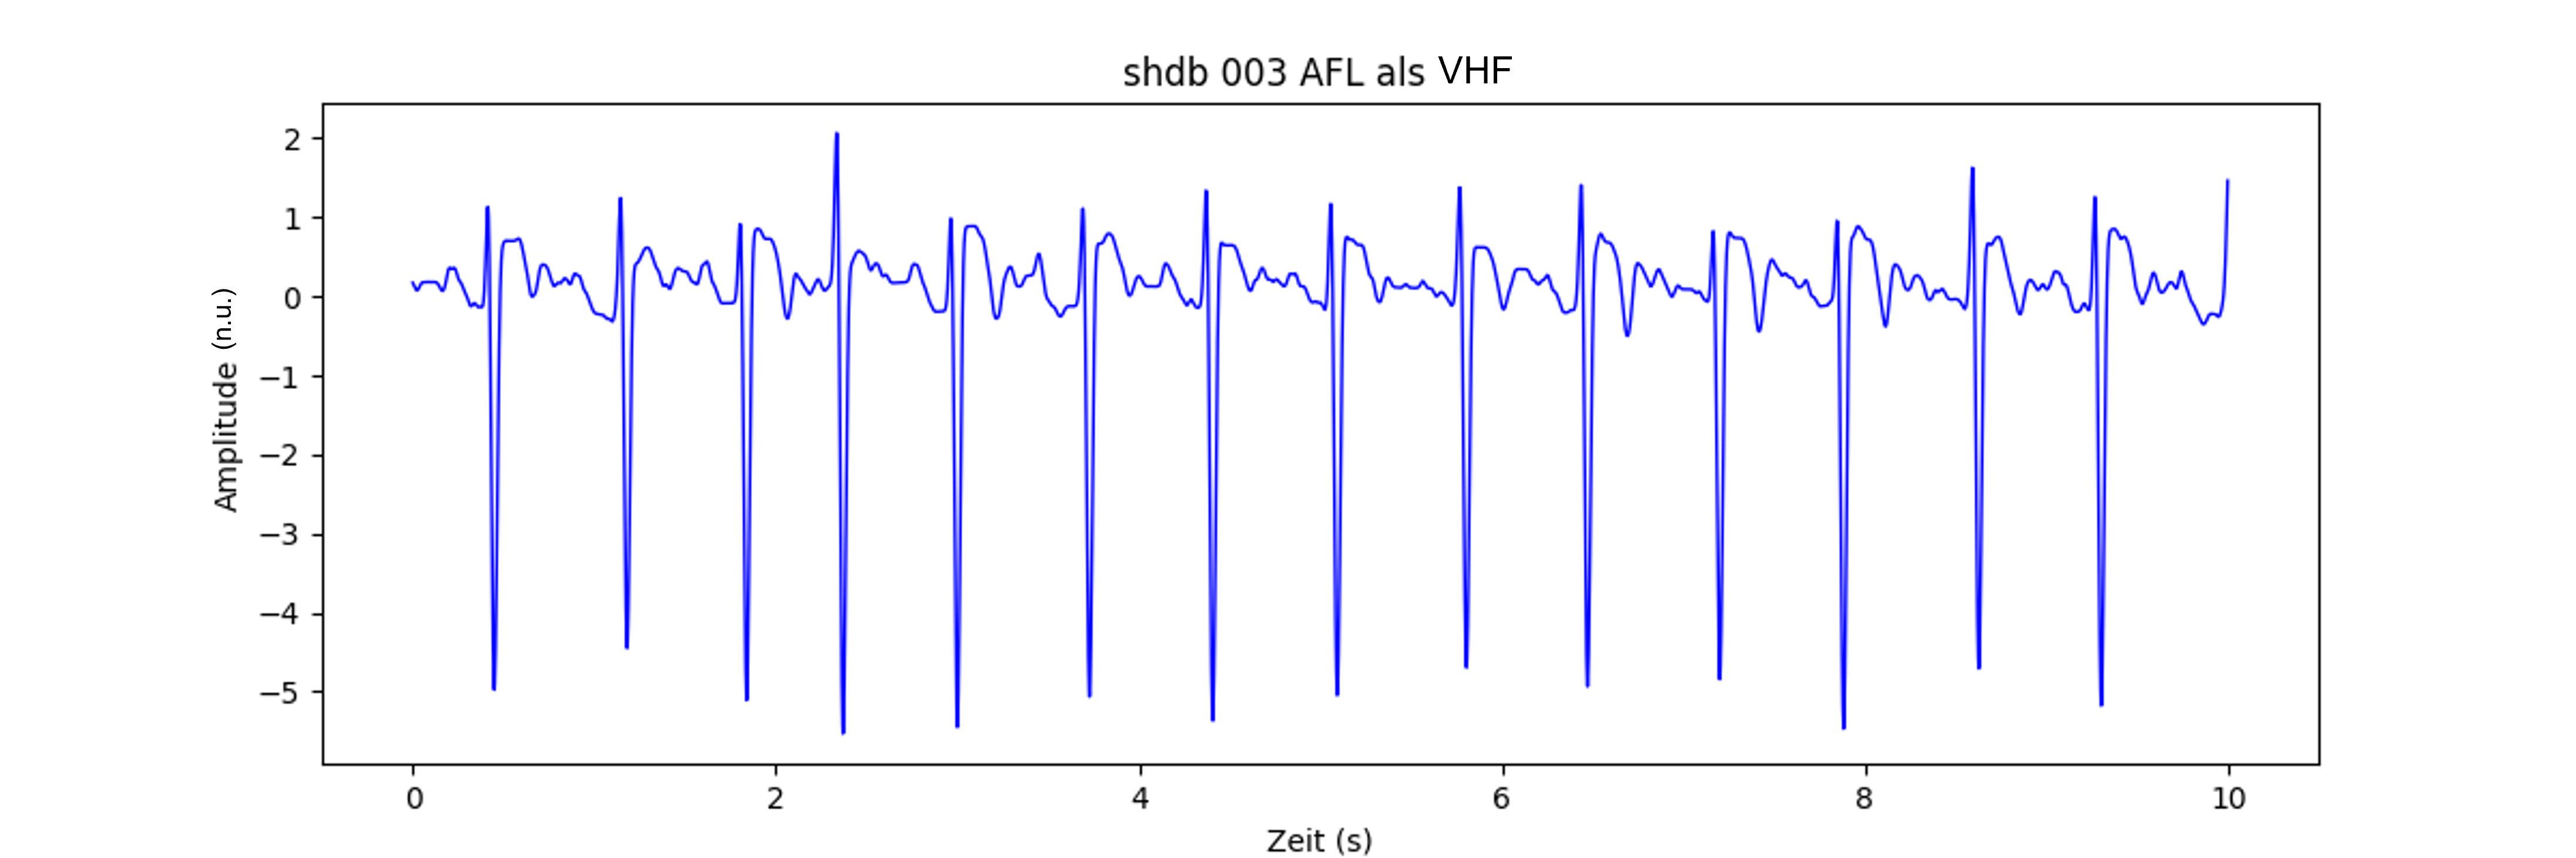
\includegraphics[width=1\textwidth]{./Bilder/003_afl.png}
\caption[SHDB-AF Aufnahme von Patient 003 mit AFL Annotation]{Eine Aufnahme von Patient 003 aus der SHDB-AF Datenbank, welche mit Vorhofflattern Annotiert und als \gls{VHF} vom gewichteten \gls{DANN} Ensemble klassifiziert wurde. Es ist keine regelmäßige Vorhoferregung zu sehen.} 
\label{fig:shdb_003_afl}
\end{figure} 

Die Klassifikation von Patient 003 erfolgte mit einem F1-Score von 0,264 für \gls{VHF} bei einer durchschnittlichen Sicherheit von 0,846. Bei diesem Patienten wurde ein mit Vorhofflattern annotierter Abschnitt vom Ensemble als \gls{VHF} klassifiziert, sowie ein mit \gls{VHF} annotierter Abschnitt nicht als \gls{VHF} detektiert. In \hyperref[fig:shdb_003_vhf]{Abb.~7.4} ist ein mit \gls{VHF} annotiertes Fenster dargestellt (welches als nicht-\gls{VHF} klassifiziert wurde), welches regelmäßige Vorhoferregungen aufweist, was auf Vorhofflattern oder Sinusrhythmus hinweist und nicht auf \gls{VHF}. In \hyperref[fig:shdb_003_afl]{Abb.~7.5} ist ein mit Vorhofflattern annotiertes Fenster dargestellt, welches als \gls{VHF} klassifiziert wurde. Hier ist keine regelmäßige Vorhoferregung zu sehen, es sind Flimmerwellen und eine leichte absolute Arrhythmie zu erkennen, sodass dies auf \gls{VHF} hinweist. Die Korrektheit der Annotationen dieser Abschnitte ist somit fraglich.


Die Klassifikation von Patient 050 erfolgte mit einem F1-Score für \gls{VHF} von 0,127 bei einer durchschnittlichen Sicherheit von 0,719. Dieser Patient besitzt insgesamt 8575 10-Sekunden-Fenster. Von diesen 8575 Fenstern sind 4 Fenster mit \gls{VHF} annotiert. Diese 4 Fenster hat das \gls{DANN} Ensemble korrekt erkannt. Auch die nicht-\gls{VHF}-Fenster wurden größtenteils korrekt klassifiziert, denn von 8571 negativen Fenstern wurden nur 55 falsch positiv klassifiziert. Durch diese starke Unausgeglichenheit der Klassen fallen jedoch selbst im Verhältnis wenige falsch positive Klassifikationen sehr stark ins Gewicht, sodass der F1-Score sehr schlecht ist. Daraus lässt sich schließen, dass der F1-Score bei unbalancierten Datensätzen keine geeignete Metrik ist.

Die Klassifikation von Patient 111 erfolgte mit einer Genauigkeit von F1~=~0,066 auf der \gls{VHF}-Klasse bei einer durchschnittlichen Sicherheit von 0,737. Bei diesem Patienten wurden Abschnitte mit Vorhoftachykardie annotiert, in denen das Ensemble \gls{VHF} detektiert. In \hyperref[fig:shdb_111_at]{Abb.~7.6} ist ein solches Fenster abgebildet. Auch hier ist die Annotation fraglich, da keine regelmäßige Vorhoferregung sichtbar und eine absolute Arrhythmie vorhanden ist.

\begin{figure}[!ht]%
\centering
	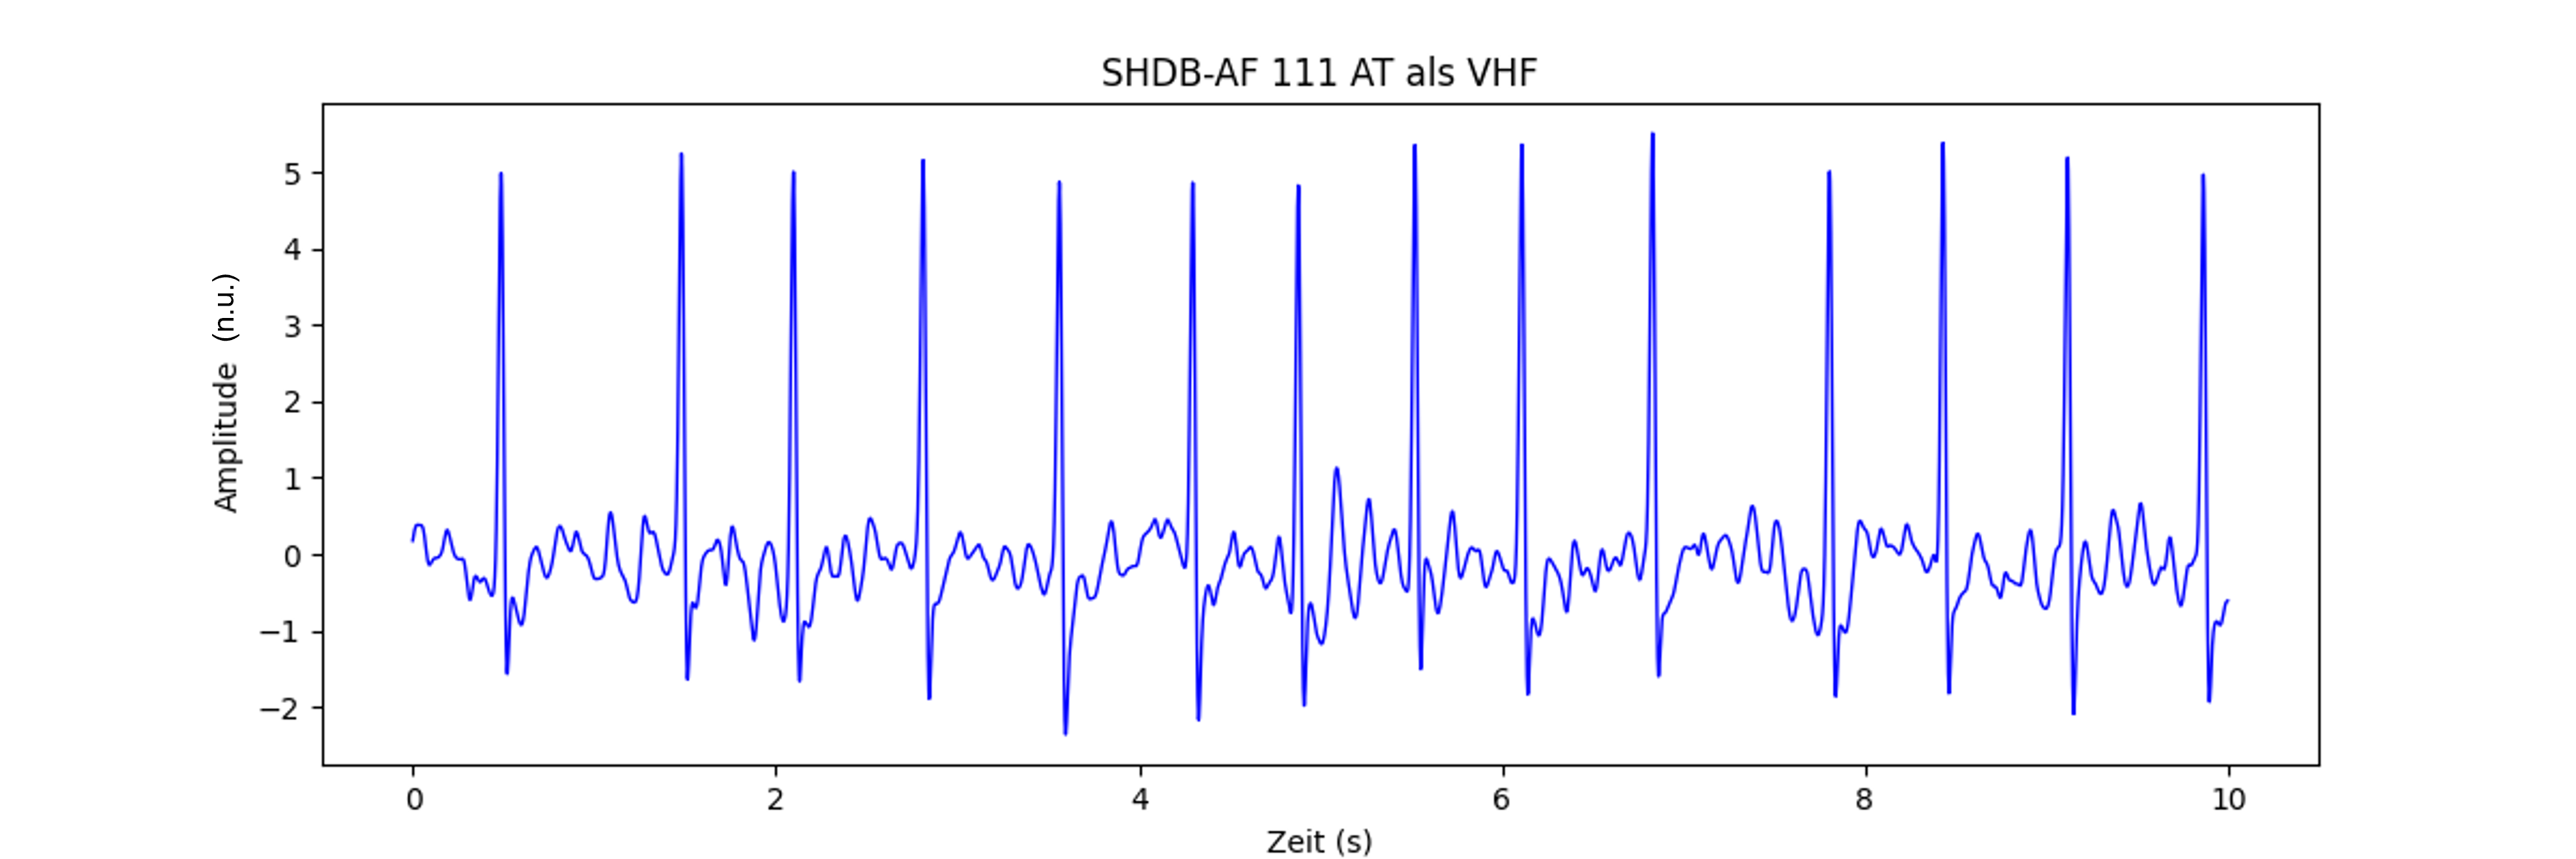
\includegraphics[width=1\textwidth]{./Bilder/111_at.png}
\caption[SHDB-AF Aufnahme von Patient 111 mit AT Annotation]{Eine Aufnahme von Patient 111 aus der SHDB-AF Datenbank, welche mit Vorhoftachkardie Annotiert und als \gls{VHF} vom gewichteten \gls{DANN} Ensemble klassifiziert wurde. Es ist keine regelmäßige Vorhoferregung zu sehen, jedoch eine absolute Arrhythmie.} 
\label{fig:shdb_111_at}
\end{figure}

\hyperref[fig:shdb_scatter_vhf]{Abb.~7.7} ist der F1-Score für die nicht-\gls{VHF}-Klasse gegen die durchschnittliche Sicherheit des Ensembles  pro Patient aufgetragen. Zusätzlich ist die Standardabweichung der Sicherheit pro Patient in Form von T-Balken eingetragen. Zu sehen ist, dass auch hier der Großteil der Teil Aufnahmen mit einem guten F1-Score und einer hohen durchschnittlichen Sicherheit klassifiziert werden konnte.

%Patient 051 hat langen Abschnitt mit N) annotiert, aber VHF detektiert (überprüfen, ob falsch annotiert)

%Patient 128 hat fast alle N abschnitte mit vhf detektiert

Die Klassifikation von Patient 024 besitzt einen F1-Score von 0,094 für die nicht-\gls{VHF}-Klasse mit einer durchschnittlichen Sicherheit von 0,606. Hier tritt derselbe Fall auf, wie bei der Klassifikation von Patient 050, mit dem Unterschied, dass Patient 024 nur drei Fenster besitzt, welche der nicht-\gls{VHF}-Klasse angehören.

Es lässt sich abschließend die Aussage treffen, dass die Klassifikation auf der SHDB-AF Datenbank zum Großteil gut funktioniert, jedoch die Gesamtgüte des Ensembles durch Aufnahmen mit einer starken Unausgeglichenheit in der Klassenverteilung und durch eventuelle falsche Annotationen reduziert wird. Aufnahmen mit einer unausgeglichenen Klassenverteilung mit vielen negativen Fällen tragen dazu bei, dass die Specificity hoch ist, da viele negative Fälle korrekt als negativ klassifiziert werden und gleichzeitig der F1-Score durch verhältnismäßig wenig falsch positive Klassifikationen verringert wird.

\begin{figure}[!ht]%
\centering
	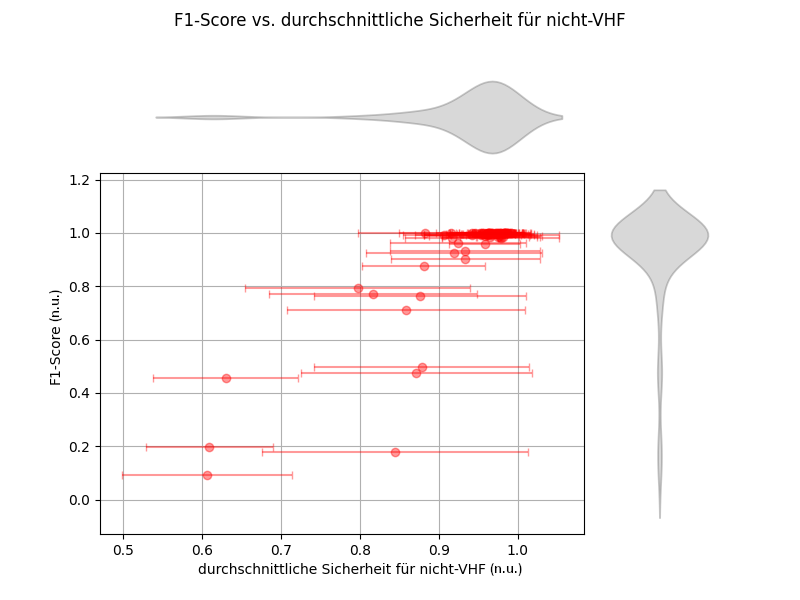
\includegraphics[width=1\textwidth]{./Bilder/shdb_plot_nicht_vhf.png}
\caption[SHDB-AF F1-Score vs. durchschnittliche Sicherheit für nicht-VHF]{F1-Score für die nicht-\gls{VHF}-Klasse gegen die durchschnittliche Sicherheit des gewichteten \gls{DANN} Ensembles pro Patient aufgetragen. Zusätzlich ist die Standardabweichung der Sicherheit pro Patient in Form von T-Balken eingetragen. Anhand des Violinenplots lässt sich die Verteilung der F1-Scores bzw. der durchschnittlichen Sicherheit für die Klassifikation über die Aufnahmen ablesen.} 
\label{fig:shdb_scatter_nvhf}
\end{figure} 

\section{Einfluss von Normalisierung}\label{sec:disknorm}

Bei der Nutzung von nicht-normalisierten Daten erzielt das gewichtete \gls{DANN} Ensemble mit einem F1-Score von 0,953 (siehe \hyperref[tab:Ergebnisse_indomain_notnorm]{Tab.~6.10}) eine minimal höhere Klassifikationsgüte auf dem Testdatensatz der Quelldomäne, als das Ensemble, welches normalisierte Daten nutzt (F1-score von 0,951, siehe \hyperref[tab:Ergebnisse_indomain]{Tab.~6.2}). Auf dem Timely Datensatz erreicht das gewichtete \gls{DANN} Ensemble ohne Normalisierung der Daten schlechtere F1-Scores (je nach Ableitung F1-Scores von 0,949-0,968 ohne Normalisierung (\hyperref[tab:Ergebnisse_timely_notnorm]{Tab.~6.11}) vs. 0,952-0,986 mit Normalisierung (\hyperref[tab:Ergebnisse_timely]{Tab.~6.6})). Daraus lässt sich schließen, dass das Unterlassen der z-Normalisierung ein Overfitting an die Trainingsdaten begünstigt.  \newpage
\chapter{Zusammenfassung und Ausblick}\label{chap:fazit}

%\section{Zusammenfassung}

In dieser Arbeit wurde ein robuster Ansatz zur Detektion von \gls{VHF} entwickelt, welcher mit \gls{EKG}s der Extremitätenableitungen aus Standard-12-Kanal-\gls{EKG}s trainiert wurde und anwendbar auf morphologisch veränderte Signale mobiler \gls{EKG}-Patches ist. 

Dazu wurden zuerst physiologische Grundlagen zu \gls{VHF}, sowie Grundlagen des \gls{DL} erarbeitet. Es wurden Ansätze zu \gls{DG} identifiziert, welche genutzt werden können, um \gls{DL}-basierte Ansätze auf unbekannte und morphologisch veränderte Signale zu übertragen. Einer dieser Ansätze ist Domain Adversarial Learning, welcher genutzt wurde, um ein \gls{DANN} auf Basis von InceptionTime zu entwickeln. Das entwickelte Modell wurde zusammen mit einem Vergleichsmodell ohne Domain Adversarial Learning auf Daten aus der Quelldomäne 12-Kanal-\gls{EKG}, sowie Daten aus der Zieldomäne mobiler \gls{EKG}-Patches angewendet. Dabei konnte gezeigt werden, dass durch Domain Adversarial Learning eine Steigerung der Klassifikationsgüte gegenüber des Vergleichsmodells sowohl auf Daten der Quelldomäne als auch auf Daten verschiedener Zieldomänen erreicht werden kann. 

%\section{Ausblick}

Eine Möglichkeit, die in der Diskussion angesprochene fehlende Erklärbarkeit zu verbessern, ist die Verbindung mit Methoden der explainable AI. Explainable AI zielt darauf ab, sogenannte Black-Box Algorithmen zu vermeiden, indem i.d.R nachträglich geschätzt wird, wie ein \gls{ANN} seine Entscheidungen trifft. 

Die Architektur des \gls{DANN}s kann weiter angepasst werden, um eine noch höhere  Klassifikationsgüte zu erzielen. Bspw. können für eine bessere Regularisierung im Label Predictor und Domain Classifier Dropout Layer eingefügt werden. Diese Schichten reduzieren Overfitting, indem zufällige Eingaben für eine bestimmte Anzahl von Neuronen auf 0 gesetzt werden. 

Die Klassifikationsgüte des Ensembles auf langen, zusammenhängenden Aufnahmen wie die der \gls{SHDB-AF}-Datenbank oder Teilen des TIMELY-Datensatzes kann unter Umständen verbessert werden, indem ein zusätzlicher Zeitfilter eingebaut wird, der nur dann ein Fenster mit \gls{VHF} klassifiziert, wenn das vorhergehende und das nachfolgende Fenster ebenso mit \gls{VHF} klassifiziert werden. Solch ein Filter würde die Robustheit gegenüber verrauschten Fenstern oder anderweitig unsicheren Detektionen erhöhen.

Abschließend lässt sich sagen, dass Domain Adversarial Learning ein sinnvoller Ansatz ist, um ein \gls{ANN} zu entwickeln, welches robust gegenüber signalmorphologischer Veränderungen ist. Das in dieser Arbeit entwickelte \gls{DANN} kann sowohl erfolgreich auf \gls{EKG}s der Extremitätenableitungen von Standard-12-Kanal-\gls{EKG}s, als auch auf unbekannte Daten mobiler \gls{EKG}-Patches angewendet werden. Somit kann es einen wertvollen Beitrag leisten, den Arbeitsaufwand von medizinischem Fachpersonal bei der Analyse von Langzeit-\gls{EKG}-Aufnahmen zu reduzieren und dazu beitragen, dass \gls{VHF} frühzeitig erkannt und damit Folgeerkrankungen vorgebeugt wird. \newpage
%Danksagung
%\input{Subfiles/tutorial.tex} \newpage
% . . .
			
			
%------------ Literaturverzeichnis -------------------------------
\pagenumbering{roman}

% Der roman counter wird mit setcounter{page}{1} vor 
% Subfiles-Einbindung auf 1 zurück gesetzt, soll aber 10 sein
% um an letzte römische Nummerierung anzuschließen
\setcounter{page}{10}

\renewcommand*{\bibname}{Quellenverzeichnis}
\printbibliography
\clearpage


%------------ Anhang ---------------------------------------------
\appendix
%Abbildungsnummerierung im Format Kapitel.Nummer
% \renewcommand{\thefigure}{\Alph{chapter}.\arabic{figure}}
% \renewcommand{\thesection}{A.\arabic{section}}
%\pagenumbering{Alph}
\addchap{Anhang}

%Hier alle eigentlichen Dateien für den Anhang einfügen
\chapter{Anhang}

\section{Suchstrings der systematischen Literaturrecherche}\label{sec:strings}

\subsection*{String 1}
\begin{verbatim}
("ECG" OR "electrocardiogra*" ) AND
("Out-of-Distribution Generalization" OR
"Out-of-Distribution Generalisation" OR "Domain Generalization" OR 
"Domain Generalisation" OR "OOD Generalization" OR "OOD Generalisation")
\end{verbatim} 

\subsection*{String 2}
\begin{verbatim}
("ECG" OR "electrocardiogra*" ) AND 
("Out-of-Distribution Generalization" OR 
"Out-of-Distribution Generalisation" OR "Domain Generalization" OR 
"Domain Generalisation" OR "OOD Generalization" OR 
"OOD Generalisation" OR "Out-of-Distribution General*" OR 
"OOD General*" OR "General* Across Domains" OR
"Cross-Domain General*" OR "Robustness to Domain Shift" OR 
"Multi-Domain Learning" OR "Domain-Invariant Learning" OR 
"Out-of-Distribution Attributes" OR "General* Target Domain" OR 
"Meta-Learning" OR "Domain Invarian*") AND 
("Neural Network" OR "Deep Learning") AND 
(classif* OR detect*)
\end{verbatim} 

\newpage
\subsection*{String 3}
\begin{verbatim}
("ECG" OR "EEG" OR "electrocardiogra*" OR 
"electroencephalogr*" OR "Biosignal" ) AND 
("Out-of-Distribution Generalization" OR 
"Out-of-Distribution Generalisation" OR "Domain Generalization" OR 
"Domain Generalisation" OR "OOD Generalization" OR 
"OOD Generalisation" OR "Out-of-Distribution General*" OR 
"OOD General*" OR "General* Across Domains" OR 
"Cross-Domain General*" OR "Robustness to Domain Shift" OR 
"Multi-Domain Learning" OR "Domain-Invariant Learning" OR 
"Out-of-Distribution Attributes" OR "General* Target Domain" OR 
"Meta-Learning" OR "Domain Invarian*") AND 
("Neural Network" OR "Deep Learning")
\end{verbatim} 

\subsection*{String 4}
\begin{verbatim}
"Medical Imaging" AND 
("Domain General*" OR "Out-of-Distribution General*" OR "OOD General*") AND
("Neural Network" OR "Deep Learning" OR "DL")
\end{verbatim} 

\newpage
\section{Grid Search Ergebnisse für InceptionTime}

\begin{table}[h!]
\centering
\caption[Ergebnisse der InceptionTime Grid Search]{Ergebnisse der Grid Search für InceptionTime. Optimierte Hyperparameter sind \texttt{depth d} (Anzahl der Inception Module), \texttt{learning rate l} und \texttt{batch size b}. Die Metriken wurden berechnet, indem vom Durchschnitt aus allen 5 Folds der Cross Validation die Standardabweichung abgezogen wurde. Die Standardabweichung $\sigma$ für die jeweilige Metrik rechts neben der betreffenden Metrik angegeben. Negative Werte kommen zustande, wenn die Standardabweichung größer als der Durchschnitt ist. Die beste Hyperparameterkombination ist hervorgehoben.}
\label{tab:GridSearch_InceptionTime}
\begin{tabular}{lcccccc}
\toprule
\textbf{Hyperparameterkombination} & \textbf{F1} & \textbf{$\sigma$} & \textbf{Sensitivität} & \textbf{$\sigma$} & \textbf{Spezifität} & \textbf{$\sigma$}\\
\midrule 
d=3 l=0,0001 b=128  & 0,919  & 0,004  & 0,928  & 0,007 & 0,903 & 0,008 \\
d=3 l=0,0001 b=64  & 0,916  & 0,005  & 0,925  & 0,008 & 0,901 & 0,007 \\
d=3 l=0,0001 b=32  & 0,919  & 0,003  & 0,925  & 0,006 & 0,910 & 0,004 \\
d=3 l=0,001	b=128  & 0,923  & 0,003  & 0,930  & 0,007 & 0,909 & 0,007 \\
d=3 l=0,001	b=64  & 0,921  & 0,004  & 0,930  & 0,007 & 0,900 & 0,011 \\
d=3 l=0,001	b=32  & 0,921  & 0,004  & 0,927  & 0,006 & 0,913 & 0,003 \\
d=3 l=0,01 b=128  & 0,920  & 0,004  & 0,928  & 0,008 & 0,905 & 0,008 \\
d=3 l=0,01 b=64  & 0,917  & 0,005  & 0,917  & 0,010 & 0,911 & 0,008 \\
d=3 l=0,01 b=32  & 0,918  & 0,005  & 0,919  & 0,015 & 0,897 & 0,015 \\
d=6 l=0,0001 b=128  & 0,930  & 0,004  & 0,935  & 0,009 & 0,913 & 0,012 \\
d=6 l=0,0001 b=64  & 0,933  & 0,002  & 0,935  & 0,006 & 0,923 & 0,008 \\
d=6 l=0,0001 b=32  & 0,932  & 0,004  & 0,937  & 0,003 & 0,926 & 0,006 \\
d=6 l=0,001 b=128  & 0,933  & 0,004  & 0,939  & 0,003 & 0,924 & 0,008 \\
d=6 l=0,001 b=64  & 0,935  & 0,003  & 0,935  & 0,007 & 0,932 & 0,004 \\
d=6 l=0,001 b=32  & 0,935  & 0,003  & 0,932  & 0,005 & 0,931 & 0,009 \\
d=6 l=0,01 b=128  & 0,934  & 0,004  & 0,935  & 0,005 & 0,932 & 0,003 \\
d=6 l=0,01 b=64  & 0,934  & 0,002  & 0,931  & 0,005 & 0,930 & 0,009 \\
d=6 l=0,01 b=32  & 0,934  & 0,003  & 0,935  & 0,007 & 0,925 & 0,008 \\
d=9 l=0,0001 b=128  & 0,938  & 0,002  & 0,933  & 0,006 & 0,933 & 0,008 \\
\textbf{d=9 l=0,0001 b=64}  & \textbf{0,939}  & \textbf{0,002}  & \textbf{0,935}  & \textbf{0,006} & \textbf{0,939} & \textbf{0,003}  \\
d=9 l=0,0001 b=32  & 0,934  & 0,004  & 0,926  & 0,013 & 0,935 & 0,006 \\
d=9 l=0,001 b=128  & 0,938  & 0,004  & 0,938  & 0,003 & 0,934 & 0,009 \\
d=9 l=0,001 b=64  & 0,939  & 0,004  & 0,938 & 0,005 & 0,937 & 0,007 \\
d=9 l=0,001 b=32  & 0,936  & 0,006  & 0,937  & 0,005 & 0,933 & 0,009 \\
d=9 l=0,01 b=128  & 0,936  & 0,004  & 0,932  & 0,005 & 0,938 & 0,006 \\
d=9 l=0,01 b=64  & 0,938  & 0,004  & 0,937  & 0,002 & 0,939 & 0,008 \\
d=9 l=0,01 b=32  & 0,934  & 0,006  & 0,924  & 0,012 & 0,939 & 0,007 \\

\bottomrule
\end{tabular}
\end{table}

						
\end{document}